% Scalar catalog source: tools/generate_scalar_instruction_catalog.py.
\section{Scalar Instruction Categories}
The scalar profile imported here is the 32-bit scalar instruction subset used by this revision. The TeX manual carries the scalar profile JSON as \path{data/scalar/scalar-instructions-32bit.json}; encoding JSON and SVG/PDF renderings are stored under \path{figs/encoding/scalar_instruction_entries}. Each instruction below gives its category, family, assembly form, encoding pattern, operand fields, encoding diagram, and description.
\begin{longtable}{@{}L{0.22\linewidth}R{0.08\linewidth}L{0.60\linewidth}@{}}
\toprule
Category & Count & Description \\
\midrule
Integer ALU and Bit-Manipulation & 60 & Integer ALU instructions compute register, immediate, word-width, bit-manipulation, multi-cycle arithmetic, max/min, and compound results. \\
Branch, Compare, and PC Control & 28 & Branch and compare instructions update control flow or materialize integer condition results using the scalar register file and PC state. \\
Load, Store, and Address Generation & 46 & Address-generation instructions calculate load/store addresses and perform scalar memory transfers through base-register, immediate, symbol, and unscaled addressing forms. \\
Atomic Memory Operations & 44 & Atomic memory operations perform load-reserved, store-conditional, swap, and arithmetic or logic read-modify-write transfers with encoded ordering qualifiers. \\
Floating-Point and Conversion & 30 & Floating-point and conversion instructions execute scalar FP arithmetic, FP compares, and integer/FP format conversions. \\
System, Cache, SSR, and Execution Control & 31 & System instructions cover cache maintenance, SSR access, architectural control, fences, traps, and bring-up or debug-oriented execution controls. \\
\bottomrule
\end{longtable}

\section{Integer ALU and Bit-Manipulation}
Integer ALU instructions compute register, immediate, word-width, bit-manipulation, multi-cycle arithmetic, max/min, and compound results.\par\smallskip
{\scriptsize
\begin{longtable}{@{}L{0.24\linewidth}R{0.09\linewidth}L{0.56\linewidth}@{}}
\toprule
Family & Count & Representative instructions \\
\midrule
Arithmetic Operation 32bit & 16 & \texttt{ADDIW, ADDW, ANDIW, ANDW, ORIW, ORW, SLLIW, SLLW} \\
Arithmetic Operation 64bit & 16 & \texttt{ADD, ADDI, AND, ANDI, OR, ORI, SLL, SLLI} \\
Bit Operation & 8 & \texttt{BCNT, BIC, BIS, BXS, BXU, CLZ, CTZ, REV} \\
Compound Operation & 1 & \texttt{CSEL} \\
Immediate & 1 & \texttt{LUI} \\
Max-Min & 4 & \texttt{MAX, MAXU, MIN, MINU} \\
Multi-Cycle ALU & 14 & \texttt{DIV, DIVU, DIVUW, DIVW, MADD, MADDW, MUL, MULU} \\
\bottomrule
\end{longtable}
}

\input{scalar-instructions/entries/003_add.tex}
\medskip
\input{scalar-instructions/entries/004_addi.tex}
\medskip
% Scalar instruction entry source: tools/generate_scalar_instruction_catalog.py.
\subsection{\texttt{ADDIW}}
\label{sec:scalar-addiw}
\index{ADDIW@\texttt{ADDIW}}
\begin{sloppypar}\noindent\textbf{Purpose.} Word (32-bit) add-immediate.\end{sloppypar}\smallskip
\noindent\textbf{Syntax.}\par
\begin{lstlisting}[style=ptoscalarcode]
addiw SrcL, uimm, ->RegDst
\end{lstlisting}
\noindent\textbf{Encoding.}\par
\noindent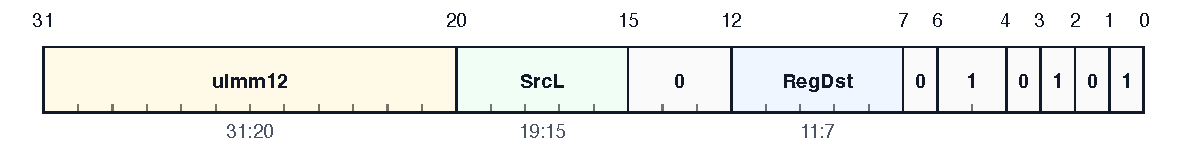
\includegraphics[width=\textwidth]{figs/encoding/scalar_instruction_entries/enc_addiw.pdf}\par\smallskip
\begin{description}[leftmargin=0.18\linewidth,style=nextline]
\item[Format] \texttt{L32} \texttt{32-bit} scalar word.
\item[Pattern] \texttt{.................000.....0110101}.
\end{description}
\noindent\textbf{Classification.}\par
\begin{description}[leftmargin=0.18\linewidth,style=nextline]
\item[Category] Integer ALU and Bit-Manipulation.
\item[Family] Arithmetic Operation 32bit.
\item[Execution class] \texttt{ALU}; uop\_kind=ALU.
\end{description}
\noindent\textbf{Operand fields.}\par
\begin{description}[leftmargin=0.18\linewidth,style=nextline]
\item[\texttt{RegDst}] Bits \texttt{11:7 (5b)}. 5-bit scalar destination register written by this instruction; X0 is hardwired to zero, so writes to X0 are ignored.
\item[\texttt{SrcL}] Bits \texttt{19:15 (5b)}. 5-bit scalar source register used as the left input operand.
\item[\texttt{uimm12}] Bits \texttt{31:20 (12b)}. 12-bit unsigned immediate operand consumed directly by the operation.
\end{description}
\noindent\textbf{Operation.}\par
\begin{lstlisting}[style=ptoscalarcode]
lhs = Read(SrcL)[31:0]
rhs = ZeroExtend(uimm)
result32 = lhs + rhs
Write(RegDst, SignExtend32(result32))
\end{lstlisting}
\Needspace{0.08\textheight}

\medskip
\input{scalar-instructions/entries/007_addw.tex}
\medskip
\input{scalar-instructions/entries/008_and.tex}
\medskip
\input{scalar-instructions/entries/009_andi.tex}
\medskip
\input{scalar-instructions/entries/010_andiw.tex}
\medskip
\input{scalar-instructions/entries/011_andw.tex}
\medskip
\input{scalar-instructions/entries/023_bcnt.tex}
\medskip
% Scalar instruction entry source: tools/generate_scalar_instruction_catalog.py.
\subsection{\texttt{BIC}}
\label{sec:scalar-bic}
\index{BIC@\texttt{BIC}}
\begin{sloppypar}\noindent\textbf{Purpose.} Bit clear / AND-NOT operation.\end{sloppypar}\smallskip
\noindent\textbf{Syntax.}\par
\begin{lstlisting}[style=ptoscalarcode]
bic SrcL, M, N, ->RegDst
\end{lstlisting}
\noindent\textbf{Encoding.}\par
\noindent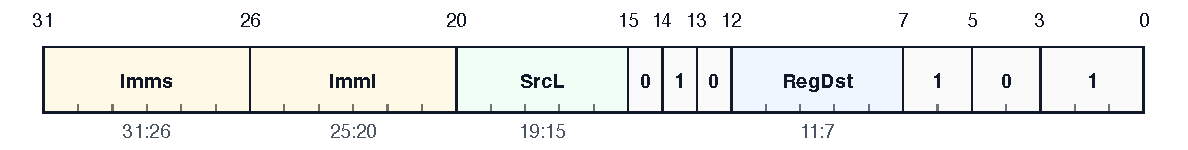
\includegraphics[width=\textwidth]{figs/encoding/scalar_instruction_entries/enc_bic.pdf}\par\smallskip
\begin{description}[leftmargin=0.18\linewidth,style=nextline]
\item[Format] \texttt{L32} \texttt{32-bit} scalar word.
\item[Pattern] \texttt{.................010.....1100111}.
\end{description}
\noindent\textbf{Classification.}\par
\begin{description}[leftmargin=0.18\linewidth,style=nextline]
\item[Category] Integer ALU and Bit-Manipulation.
\item[Family] Bit Operation.
\item[Execution class] \texttt{ALU}; uop\_kind=ALU.
\end{description}
\noindent\textbf{Operand fields.}\par
\begin{description}[leftmargin=0.18\linewidth,style=nextline]
\item[\texttt{RegDst}] Bits \texttt{11:7 (5b)}. 5-bit scalar destination register written by this instruction; X0 is hardwired to zero, so writes to X0 are ignored.
\item[\texttt{SrcL}] Bits \texttt{19:15 (5b)}. 5-bit scalar source register used as the left input operand.
\item[\texttt{imml}] Bits \texttt{25:20 (6b)}. 6-bit unsigned immediate operand consumed directly by the operation.
\item[\texttt{imms}] Bits \texttt{31:26 (6b)}. 6-bit unsigned immediate operand consumed directly by the operation.
\end{description}
\noindent\textbf{Operation.}\par
\begin{lstlisting}[style=ptoscalarcode]
mask = BitMask(M, N)
Write(RegDst, Read(SrcL) & ~mask)
\end{lstlisting}
\Needspace{0.08\textheight}

\medskip
\input{scalar-instructions/entries/025_bis.tex}
\medskip
\input{scalar-instructions/entries/030_bxs.tex}
\medskip
% Scalar instruction entry source: tools/generate_scalar_instruction_catalog.py.
\subsection{\texttt{BXU}}
\label{sec:scalar-bxu}
\index{BXU@\texttt{BXU}}
\begin{sloppypar}\noindent\textbf{Purpose.} Bit-field extract (unsigned).\end{sloppypar}\smallskip
\noindent\textbf{Syntax.}\par
\begin{lstlisting}[style=ptoscalarcode]
bxu SrcL, M, N, ->RegDst
\end{lstlisting}
\noindent\textbf{Encoding.}\par
\noindent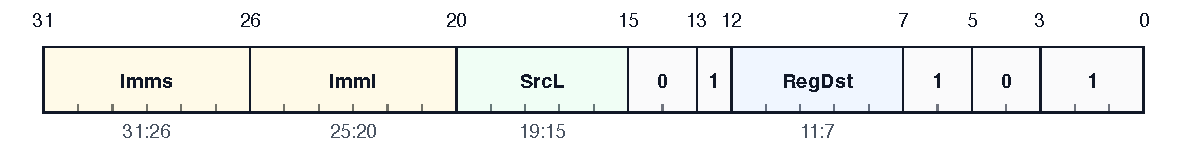
\includegraphics[width=\textwidth]{figs/encoding/scalar_instruction_entries/enc_bxu.pdf}\par\smallskip
\begin{description}[leftmargin=0.18\linewidth,style=nextline]
\item[Format] \texttt{L32} \texttt{32-bit} scalar word.
\item[Pattern] \texttt{.................001.....1100111}.
\end{description}
\noindent\textbf{Classification.}\par
\begin{description}[leftmargin=0.18\linewidth,style=nextline]
\item[Category] Integer ALU and Bit-Manipulation.
\item[Family] Bit Operation.
\item[Execution class] \texttt{ALU}; uop\_kind=ALU.
\end{description}
\noindent\textbf{Operand fields.}\par
\begin{description}[leftmargin=0.18\linewidth,style=nextline]
\item[\texttt{RegDst}] Bits \texttt{11:7 (5b)}. 5-bit scalar destination register written by this instruction; X0 is hardwired to zero, so writes to X0 are ignored.
\item[\texttt{SrcL}] Bits \texttt{19:15 (5b)}. 5-bit scalar source register used as the left input operand.
\item[\texttt{imml}] Bits \texttt{25:20 (6b)}. 6-bit unsigned immediate operand consumed directly by the operation.
\item[\texttt{imms}] Bits \texttt{31:26 (6b)}. 6-bit unsigned immediate operand consumed directly by the operation.
\end{description}
\noindent\textbf{Operation.}\par
\begin{lstlisting}[style=ptoscalarcode]
field = ExtractBits(Read(SrcL), M, N)
Write(RegDst, ZeroExtend(field))
\end{lstlisting}
\Needspace{0.08\textheight}

\medskip
% Scalar instruction entry source: tools/generate_scalar_instruction_catalog.py.
\subsection{\texttt{CLZ}}
\label{sec:scalar-clz}
\index{CLZ@\texttt{CLZ}}
\begin{sloppypar}\noindent\textbf{Purpose.} Count leading zeros.\end{sloppypar}\smallskip
\noindent\textbf{Syntax.}\par
\begin{lstlisting}[style=ptoscalarcode]
clz SrcL,  M, N, ->RegDst
\end{lstlisting}
\noindent\textbf{Encoding.}\par
\noindent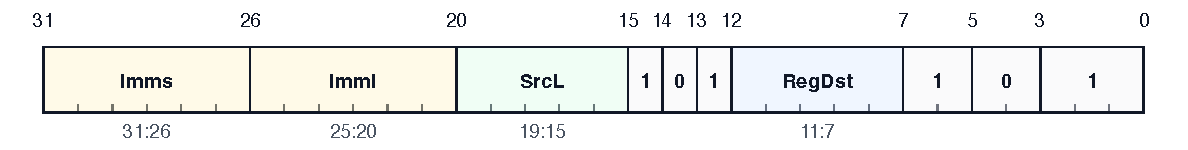
\includegraphics[width=\textwidth]{figs/encoding/scalar_instruction_entries/enc_clz.pdf}\par\smallskip
\begin{description}[leftmargin=0.18\linewidth,style=nextline]
\item[Format] \texttt{L32} \texttt{32-bit} scalar word.
\item[Pattern] \texttt{.................101.....1100111}.
\end{description}
\noindent\textbf{Classification.}\par
\begin{description}[leftmargin=0.18\linewidth,style=nextline]
\item[Category] Integer ALU and Bit-Manipulation.
\item[Family] Bit Operation.
\item[Execution class] \texttt{ALU}; uop\_kind=ALU.
\end{description}
\noindent\textbf{Operand fields.}\par
\begin{description}[leftmargin=0.18\linewidth,style=nextline]
\item[\texttt{RegDst}] Bits \texttt{11:7 (5b)}. 5-bit scalar destination register written by this instruction; X0 is hardwired to zero, so writes to X0 are ignored.
\item[\texttt{SrcL}] Bits \texttt{19:15 (5b)}. 5-bit scalar source register used as the left input operand.
\item[\texttt{imml}] Bits \texttt{25:20 (6b)}. 6-bit unsigned immediate operand consumed directly by the operation.
\item[\texttt{imms}] Bits \texttt{31:26 (6b)}. 6-bit unsigned immediate operand consumed directly by the operation.
\end{description}
\noindent\textbf{Operation.}\par
\begin{lstlisting}[style=ptoscalarcode]
field = ExtractBits(Read(SrcL), M, N)
Write(RegDst, CountLeadingZeros(field))
\end{lstlisting}
\Needspace{0.08\textheight}

\medskip
% Scalar instruction entry source: tools/generate_scalar_instruction_catalog.py.
\subsection{\texttt{CSEL}}
\label{sec:scalar-csel}
\index{CSEL@\texttt{CSEL}}
\begin{sloppypar}\noindent\textbf{Purpose.} Conditional select.\end{sloppypar}\smallskip
\noindent\textbf{Syntax.}\par
\begin{lstlisting}[style=ptoscalarcode]
csel SrcP, SrcL, SrcR<.neg>, ->RegDst
\end{lstlisting}
\noindent\textbf{Encoding.}\par
\noindent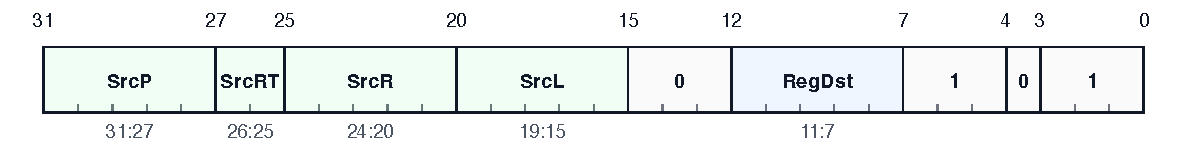
\includegraphics[width=\textwidth]{figs/encoding/scalar_instruction_entries/enc_csel.pdf}\par\smallskip
\begin{description}[leftmargin=0.18\linewidth,style=nextline]
\item[Format] \texttt{L32} \texttt{32-bit} scalar word.
\item[Pattern] \texttt{.................000.....1110111}.
\end{description}
\noindent\textbf{Classification.}\par
\begin{description}[leftmargin=0.18\linewidth,style=nextline]
\item[Category] Integer ALU and Bit-Manipulation.
\item[Family] Compound Operation.
\item[Execution class] \texttt{ALU}; uop\_kind=ALU.
\end{description}
\noindent\textbf{Operand fields.}\par
\begin{description}[leftmargin=0.18\linewidth,style=nextline]
\item[\texttt{RegDst}] Bits \texttt{11:7 (5b)}. 5-bit scalar destination register written by this instruction; X0 is hardwired to zero, so writes to X0 are ignored.
\item[\texttt{SrcL}] Bits \texttt{19:15 (5b)}. 5-bit scalar source register used as the left input operand.
\item[\texttt{SrcP}] Bits \texttt{31:27 (5b)}. 5-bit scalar source register supplying the predicate or condition input used by the conditional select operation.
\item[\texttt{SrcR}] Bits \texttt{24:20 (5b)}. 5-bit scalar source register used as the right input operand before any encoded modifier or shift is applied.
\item[\texttt{SrcRType}] Bits \texttt{26:25 (2b)}. 2-bit modifier for SrcR. It selects the encoded source form shown in the syntax, such as signed-word, unsigned-word, negated, or unmodified register input.
\end{description}
\noindent\textbf{Operation.}\par
\begin{lstlisting}[style=ptoscalarcode]
p = Read(SrcP)
lhs = Read(SrcL)
rhs = Read(SrcR)  // apply optional .neg as encoded
result = (p != 0) ? lhs : rhs
Write(RegDst, result)
\end{lstlisting}
\Needspace{0.08\textheight}

\medskip
\input{scalar-instructions/entries/050_ctz.tex}
\medskip
\input{scalar-instructions/entries/059_div.tex}
\medskip
\input{scalar-instructions/entries/060_divu.tex}
\medskip
\input{scalar-instructions/entries/061_divuw.tex}
\medskip
\input{scalar-instructions/entries/062_divw.tex}
\medskip
% Scalar instruction entry source: tools/generate_scalar_instruction_catalog.py.
\subsection{\texttt{LUI}}
\label{sec:scalar-lui}
\index{LUI@\texttt{LUI}}
\begin{sloppypar}\noindent\textbf{Purpose.} Load upper immediate (constant materialization).\end{sloppypar}\smallskip
\noindent\textbf{Syntax.}\par
\begin{lstlisting}[style=ptoscalarcode]
lui simm, ->RegDst
\end{lstlisting}
\noindent\textbf{Encoding.}\par
\noindent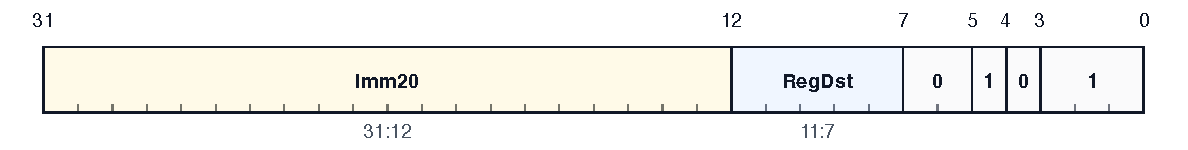
\includegraphics[width=\textwidth]{figs/encoding/scalar_instruction_entries/enc_lui.pdf}\par\smallskip
\begin{description}[leftmargin=0.18\linewidth,style=nextline]
\item[Format] \texttt{L32} \texttt{32-bit} scalar word.
\item[Pattern] \texttt{.........................0010111}.
\end{description}
\noindent\textbf{Classification.}\par
\begin{description}[leftmargin=0.18\linewidth,style=nextline]
\item[Category] Integer ALU and Bit-Manipulation.
\item[Family] Immediate.
\item[Execution class] \texttt{ALU}; uop\_kind=ALU.
\end{description}
\noindent\textbf{Operand fields.}\par
\begin{description}[leftmargin=0.18\linewidth,style=nextline]
\item[\texttt{RegDst}] Bits \texttt{11:7 (5b)}. 5-bit scalar destination register that receives the loaded value after any sign or zero extension; X0 discards the load result.
\item[\texttt{imm20}] Bits \texttt{31:12 (20b)}. 20-bit unsigned immediate operand consumed directly by the operation.
\end{description}
\noindent\textbf{Operation.}\par
\begin{lstlisting}[style=ptoscalarcode]
imm = (SignExtend(imm20) << 12)
Write(RegDst, imm)
\end{lstlisting}
\Needspace{0.08\textheight}

\medskip
% Scalar instruction entry source: tools/generate_scalar_instruction_catalog.py.
\subsection{\texttt{MADD}}
\label{sec:scalar-madd}
\index{MADD@\texttt{MADD}}
\begin{sloppypar}\noindent\textbf{Purpose.} Multiply-add (three-source).\end{sloppypar}\smallskip
\noindent\textbf{Syntax.}\par
\begin{lstlisting}[style=ptoscalarcode]
madd SrcL, SrcR, SrcD, ->RegDst
\end{lstlisting}
\noindent\textbf{Encoding.}\par
\noindent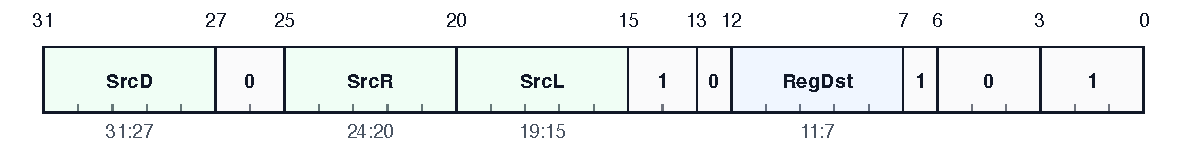
\includegraphics[width=\textwidth]{figs/encoding/scalar_instruction_entries/enc_madd.pdf}\par\smallskip
\begin{description}[leftmargin=0.18\linewidth,style=nextline]
\item[Format] \texttt{L32} \texttt{32-bit} scalar word.
\item[Pattern] \texttt{.....00..........110.....1000111}.
\end{description}
\noindent\textbf{Classification.}\par
\begin{description}[leftmargin=0.18\linewidth,style=nextline]
\item[Category] Integer ALU and Bit-Manipulation.
\item[Family] Multi-Cycle ALU.
\item[Execution class] \texttt{ALU}; uop\_kind=ALU, alu\_kind=ALU\_MULTI\_CYCLE.
\end{description}
\noindent\textbf{Operand fields.}\par
\begin{description}[leftmargin=0.18\linewidth,style=nextline]
\item[\texttt{RegDst}] Bits \texttt{11:7 (5b)}. 5-bit scalar destination register written by this instruction; X0 is hardwired to zero, so writes to X0 are ignored.
\item[\texttt{SrcD}] Bits \texttt{31:27 (5b)}. 5-bit scalar source register containing the data operand consumed by the instruction.
\item[\texttt{SrcL}] Bits \texttt{19:15 (5b)}. 5-bit scalar source register used as the left input operand.
\item[\texttt{SrcR}] Bits \texttt{24:20 (5b)}. 5-bit scalar source register used as the right input operand before any encoded modifier or shift is applied.
\end{description}
\noindent\textbf{Operation.}\par
\begin{lstlisting}[style=ptoscalarcode]
a = Read(SrcL)
b = Read(SrcR)
d = Read(SrcD)
result = LowProduct(a, b) + d
Write(RegDst, result)
\end{lstlisting}
\Needspace{0.08\textheight}

\medskip
\input{scalar-instructions/entries/147_maddw.tex}
\medskip
\input{scalar-instructions/entries/148_max.tex}
\medskip
\input{scalar-instructions/entries/149_maxu.tex}
\medskip
\input{scalar-instructions/entries/150_min.tex}
\medskip
% Scalar instruction entry source: tools/generate_scalar_instruction_catalog.py.
\subsection{\texttt{MINU}}
\label{sec:scalar-minu}
\index{MINU@\texttt{MINU}}
\begin{sloppypar}\noindent\textbf{Purpose.} Performs the operation indicated by the mnemonic on the operands specified by the selected form. Operand-size, signedness, and addressing modifiers are encoded via suffixes and qualifiers in the assembly syntax.\end{sloppypar}\smallskip
\noindent\textbf{Syntax.}\par
\begin{lstlisting}[style=ptoscalarcode]
minu SrcL, SrcR, ->RegDst
\end{lstlisting}
\noindent\textbf{Encoding.}\par
\noindent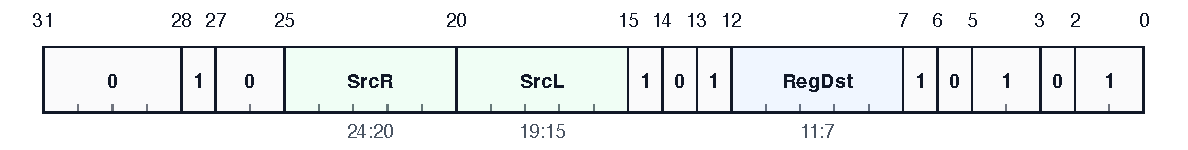
\includegraphics[width=\textwidth]{figs/encoding/scalar_instruction_entries/enc_minu.pdf}\par\smallskip
\begin{description}[leftmargin=0.18\linewidth,style=nextline]
\item[Format] \texttt{L32} \texttt{32-bit} scalar word.
\item[Pattern] \texttt{0000100..........101.....1011011}.
\end{description}
\noindent\textbf{Classification.}\par
\begin{description}[leftmargin=0.18\linewidth,style=nextline]
\item[Category] Integer ALU and Bit-Manipulation.
\item[Family] Max-Min.
\item[Execution class] \texttt{ALU}; uop\_kind=ALU.
\end{description}
\noindent\textbf{Operand fields.}\par
\begin{description}[leftmargin=0.18\linewidth,style=nextline]
\item[\texttt{RegDst}] Bits \texttt{11:7 (5b)}. 5-bit scalar destination register written by this instruction; X0 is hardwired to zero, so writes to X0 are ignored.
\item[\texttt{SrcL}] Bits \texttt{19:15 (5b)}. 5-bit scalar source register used as the left input operand.
\item[\texttt{SrcR}] Bits \texttt{24:20 (5b)}. 5-bit scalar source register used as the right input operand before any encoded modifier or shift is applied.
\end{description}
\noindent\textbf{Operation.}\par
\begin{lstlisting}[style=ptoscalarcode]
a = Read(SrcL)
b = Read(SrcR)
result = (unsigned(a) <= unsigned(b)) ? a : b
Write(RegDst, result)
\end{lstlisting}
\Needspace{0.08\textheight}

\medskip
\input{scalar-instructions/entries/152_mul.tex}
\medskip
\input{scalar-instructions/entries/153_mulu.tex}
\medskip
\input{scalar-instructions/entries/154_muluw.tex}
\medskip
% Scalar instruction entry source: tools/generate_scalar_instruction_catalog.py.
\subsection{\texttt{MULW}}
\label{sec:scalar-mulw}
\index{MULW@\texttt{MULW}}
\begin{sloppypar}\noindent\textbf{Purpose.} Word (32-bit) integer multiply.\end{sloppypar}\smallskip
\noindent\textbf{Syntax.}\par
\begin{lstlisting}[style=ptoscalarcode]
mulw SrcL, SrcR, ->RegDst
\end{lstlisting}
\noindent\textbf{Encoding.}\par
\noindent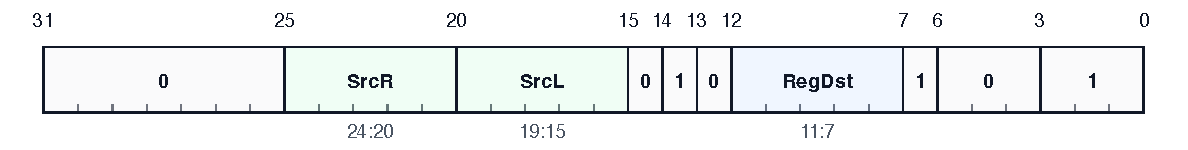
\includegraphics[width=\textwidth]{figs/encoding/scalar_instruction_entries/enc_mulw.pdf}\par\smallskip
\begin{description}[leftmargin=0.18\linewidth,style=nextline]
\item[Format] \texttt{L32} \texttt{32-bit} scalar word.
\item[Pattern] \texttt{0000000..........010.....1000111}.
\end{description}
\noindent\textbf{Classification.}\par
\begin{description}[leftmargin=0.18\linewidth,style=nextline]
\item[Category] Integer ALU and Bit-Manipulation.
\item[Family] Multi-Cycle ALU.
\item[Execution class] \texttt{ALU}; uop\_kind=ALU, alu\_kind=ALU\_MULTI\_CYCLE.
\end{description}
\noindent\textbf{Operand fields.}\par
\begin{description}[leftmargin=0.18\linewidth,style=nextline]
\item[\texttt{RegDst}] Bits \texttt{11:7 (5b)}. 5-bit scalar destination register written by this instruction; X0 is hardwired to zero, so writes to X0 are ignored.
\item[\texttt{SrcL}] Bits \texttt{19:15 (5b)}. 5-bit scalar source register used as the left input operand.
\item[\texttt{SrcR}] Bits \texttt{24:20 (5b)}. 5-bit scalar source register used as the right input operand before any encoded modifier or shift is applied.
\end{description}
\noindent\textbf{Operation.}\par
\begin{lstlisting}[style=ptoscalarcode]
a = Read(SrcL)[31:0]
b = Read(SrcR)[31:0]
result = LowProduct(a, b)
result = SignExtend32(result)
Write(RegDst, result)
\end{lstlisting}
\Needspace{0.08\textheight}

\medskip
% Scalar instruction entry source: tools/generate_scalar_instruction_catalog.py.
\subsection{\texttt{OR}}
\label{sec:scalar-or}
\index{OR@\texttt{OR}}
\begin{sloppypar}\noindent\textbf{Purpose.} Bitwise OR.\end{sloppypar}\smallskip
\noindent\textbf{Syntax.}\par
\begin{lstlisting}[style=ptoscalarcode]
or SrcL, SrcR<{.sw,.uw,.not}><<<shamt>, ->RegDst
\end{lstlisting}
\noindent\textbf{Encoding.}\par
\noindent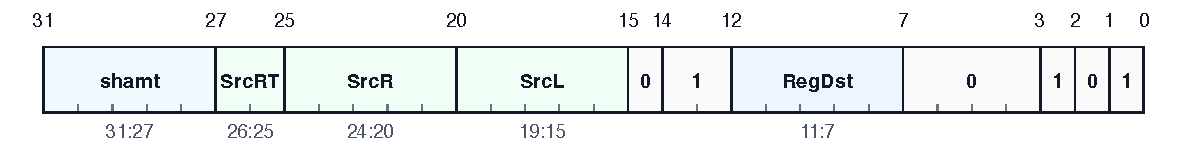
\includegraphics[width=\textwidth]{figs/encoding/scalar_instruction_entries/enc_or.pdf}\par\smallskip
\begin{description}[leftmargin=0.18\linewidth,style=nextline]
\item[Format] \texttt{L32} \texttt{32-bit} scalar word.
\item[Pattern] \texttt{.................011.....0000101}.
\end{description}
\noindent\textbf{Classification.}\par
\begin{description}[leftmargin=0.18\linewidth,style=nextline]
\item[Category] Integer ALU and Bit-Manipulation.
\item[Family] Arithmetic Operation 64bit.
\item[Execution class] \texttt{ALU}; uop\_kind=ALU.
\end{description}
\noindent\textbf{Operand fields.}\par
\begin{description}[leftmargin=0.18\linewidth,style=nextline]
\item[\texttt{RegDst}] Bits \texttt{11:7 (5b)}. 5-bit scalar destination register written by this instruction; X0 is hardwired to zero, so writes to X0 are ignored.
\item[\texttt{SrcL}] Bits \texttt{19:15 (5b)}. 5-bit scalar source register used as the left input operand.
\item[\texttt{SrcR}] Bits \texttt{24:20 (5b)}. 5-bit scalar source register used as the right input operand before any encoded modifier or shift is applied.
\item[\texttt{SrcRType}] Bits \texttt{26:25 (2b)}. 2-bit modifier for SrcR. It selects the encoded source form shown in the syntax, such as signed-word, unsigned-word, negated, or unmodified register input.
\item[\texttt{shamt}] Bits \texttt{31:27 (5b)}. 5-bit shift amount applied to the modified right operand before the ALU or address calculation uses it.
\end{description}
\noindent\textbf{Operation.}\par
\begin{lstlisting}[style=ptoscalarcode]
lhs = Read(SrcL)
rhs = Read(SrcR)  // apply modifiers/shift as encoded
result = lhs | rhs
Write(RegDst, result)
\end{lstlisting}
\Needspace{0.08\textheight}

\medskip
% Scalar instruction entry source: tools/generate_scalar_instruction_catalog.py.
\subsection{\texttt{ORI}}
\label{sec:scalar-ori}
\index{ORI@\texttt{ORI}}
\begin{sloppypar}\noindent\textbf{Purpose.} Bitwise OR (immediate).\end{sloppypar}\smallskip
\noindent\textbf{Syntax.}\par
\begin{lstlisting}[style=ptoscalarcode]
ori SrcL, simm, ->RegDst
\end{lstlisting}
\noindent\textbf{Encoding.}\par
\noindent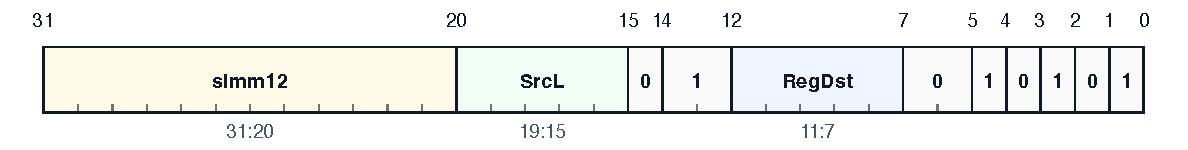
\includegraphics[width=\textwidth]{figs/encoding/scalar_instruction_entries/enc_ori.pdf}\par\smallskip
\begin{description}[leftmargin=0.18\linewidth,style=nextline]
\item[Format] \texttt{L32} \texttt{32-bit} scalar word.
\item[Pattern] \texttt{.................011.....0010101}.
\end{description}
\noindent\textbf{Classification.}\par
\begin{description}[leftmargin=0.18\linewidth,style=nextline]
\item[Category] Integer ALU and Bit-Manipulation.
\item[Family] Arithmetic Operation 64bit.
\item[Execution class] \texttt{ALU}; uop\_kind=ALU.
\end{description}
\noindent\textbf{Operand fields.}\par
\begin{description}[leftmargin=0.18\linewidth,style=nextline]
\item[\texttt{RegDst}] Bits \texttt{11:7 (5b)}. 5-bit scalar destination register written by this instruction; X0 is hardwired to zero, so writes to X0 are ignored.
\item[\texttt{SrcL}] Bits \texttt{19:15 (5b)}. 5-bit scalar source register used as the left input operand.
\item[\texttt{simm12}] Bits \texttt{31:20 (12b)}. 12-bit signed immediate operand that is sign-extended before use.
\end{description}
\noindent\textbf{Operation.}\par
\begin{lstlisting}[style=ptoscalarcode]
a = Read(SrcL)
imm = SignExtend(simm12)
result = a | imm
Write(RegDst, result)
\end{lstlisting}
\Needspace{0.08\textheight}

\medskip
% Scalar instruction entry source: tools/generate_scalar_instruction_catalog.py.
\subsection{\texttt{ORIW}}
\label{sec:scalar-oriw}
\index{ORIW@\texttt{ORIW}}
\begin{sloppypar}\noindent\textbf{Purpose.} Word (32-bit) OR-immediate.\end{sloppypar}\smallskip
\noindent\textbf{Syntax.}\par
\begin{lstlisting}[style=ptoscalarcode]
oriw SrcL, simm, ->RegDst
\end{lstlisting}
\noindent\textbf{Encoding.}\par
\noindent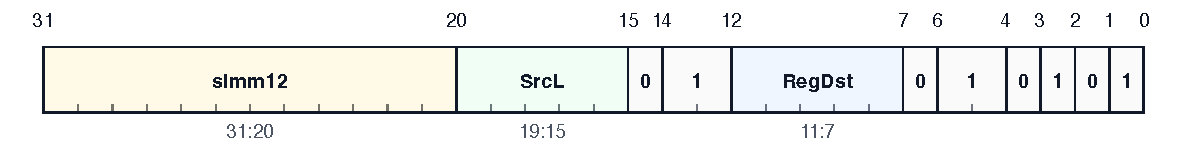
\includegraphics[width=\textwidth]{figs/encoding/scalar_instruction_entries/enc_oriw.pdf}\par\smallskip
\begin{description}[leftmargin=0.18\linewidth,style=nextline]
\item[Format] \texttt{L32} \texttt{32-bit} scalar word.
\item[Pattern] \texttt{.................011.....0110101}.
\end{description}
\noindent\textbf{Classification.}\par
\begin{description}[leftmargin=0.18\linewidth,style=nextline]
\item[Category] Integer ALU and Bit-Manipulation.
\item[Family] Arithmetic Operation 32bit.
\item[Execution class] \texttt{ALU}; uop\_kind=ALU.
\end{description}
\noindent\textbf{Operand fields.}\par
\begin{description}[leftmargin=0.18\linewidth,style=nextline]
\item[\texttt{RegDst}] Bits \texttt{11:7 (5b)}. 5-bit scalar destination register written by this instruction; X0 is hardwired to zero, so writes to X0 are ignored.
\item[\texttt{SrcL}] Bits \texttt{19:15 (5b)}. 5-bit scalar source register used as the left input operand.
\item[\texttt{simm12}] Bits \texttt{31:20 (12b)}. 12-bit signed immediate operand that is sign-extended before use.
\end{description}
\noindent\textbf{Operation.}\par
\begin{lstlisting}[style=ptoscalarcode]
a = Read(SrcL)[31:0]
imm = SignExtend(simm12)[31:0]
result32 = a | imm
result = SignExtend32(result32)
Write(RegDst, result)
\end{lstlisting}
\Needspace{0.08\textheight}

\medskip
\input{scalar-instructions/entries/159_orw.tex}
\medskip
% Scalar instruction entry source: tools/generate_scalar_instruction_catalog.py.
\subsection{\texttt{REM}}
\label{sec:scalar-rem}
\index{REM@\texttt{REM}}
\begin{sloppypar}\noindent\textbf{Purpose.} Integer remainder (signed).\end{sloppypar}\smallskip
\noindent\textbf{Syntax.}\par
\begin{lstlisting}[style=ptoscalarcode]
rem SrcL, SrcR, ->RegDst
\end{lstlisting}
\noindent\textbf{Encoding.}\par
\noindent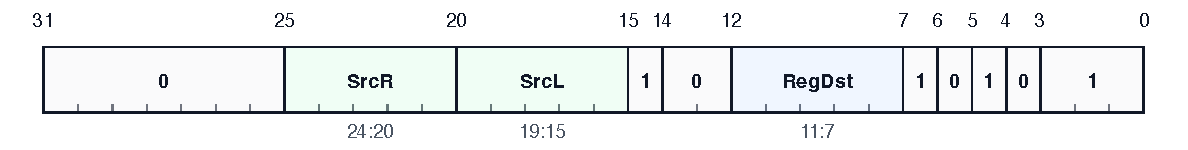
\includegraphics[width=\textwidth]{figs/encoding/scalar_instruction_entries/enc_rem.pdf}\par\smallskip
\begin{description}[leftmargin=0.18\linewidth,style=nextline]
\item[Format] \texttt{L32} \texttt{32-bit} scalar word.
\item[Pattern] \texttt{0000000..........100.....1010111}.
\end{description}
\noindent\textbf{Classification.}\par
\begin{description}[leftmargin=0.18\linewidth,style=nextline]
\item[Category] Integer ALU and Bit-Manipulation.
\item[Family] Multi-Cycle ALU.
\item[Execution class] \texttt{ALU}; uop\_kind=ALU, alu\_kind=ALU\_MULTI\_CYCLE.
\end{description}
\noindent\textbf{Operand fields.}\par
\begin{description}[leftmargin=0.18\linewidth,style=nextline]
\item[\texttt{RegDst}] Bits \texttt{11:7 (5b)}. 5-bit scalar destination register written by this instruction; X0 is hardwired to zero, so writes to X0 are ignored.
\item[\texttt{SrcL}] Bits \texttt{19:15 (5b)}. 5-bit scalar source register used as the left input operand.
\item[\texttt{SrcR}] Bits \texttt{24:20 (5b)}. 5-bit scalar source register used as the right input operand before any encoded modifier or shift is applied.
\end{description}
\noindent\textbf{Operation.}\par
\begin{lstlisting}[style=ptoscalarcode]
a = Read(SrcL)
b = Read(SrcR)
if (b == 0):
  result = a
else:
  // signed overflow: MIN_INT / -1
  q = TruncTowardZeroDiv(a, b)
  result = a - q*b
Write(RegDst, result)
\end{lstlisting}
\Needspace{0.08\textheight}

\medskip
\input{scalar-instructions/entries/163_remu.tex}
\medskip
\input{scalar-instructions/entries/164_remuw.tex}
\medskip
% Scalar instruction entry source: tools/generate_scalar_instruction_catalog.py.
\subsection{\texttt{REMW}}
\label{sec:scalar-remw}
\index{REMW@\texttt{REMW}}
\begin{sloppypar}\noindent\textbf{Purpose.} Word (32-bit) integer remainder (signed).\end{sloppypar}\smallskip
\noindent\textbf{Syntax.}\par
\begin{lstlisting}[style=ptoscalarcode]
remw SrcL, SrcR, ->RegDst
\end{lstlisting}
\noindent\textbf{Encoding.}\par
\noindent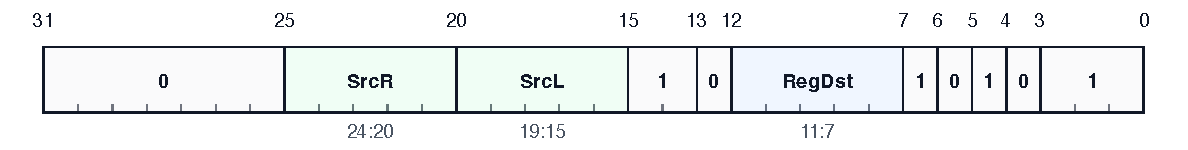
\includegraphics[width=\textwidth]{figs/encoding/scalar_instruction_entries/enc_remw.pdf}\par\smallskip
\begin{description}[leftmargin=0.18\linewidth,style=nextline]
\item[Format] \texttt{L32} \texttt{32-bit} scalar word.
\item[Pattern] \texttt{0000000..........110.....1010111}.
\end{description}
\noindent\textbf{Classification.}\par
\begin{description}[leftmargin=0.18\linewidth,style=nextline]
\item[Category] Integer ALU and Bit-Manipulation.
\item[Family] Multi-Cycle ALU.
\item[Execution class] \texttt{ALU}; uop\_kind=ALU, alu\_kind=ALU\_MULTI\_CYCLE.
\end{description}
\noindent\textbf{Operand fields.}\par
\begin{description}[leftmargin=0.18\linewidth,style=nextline]
\item[\texttt{RegDst}] Bits \texttt{11:7 (5b)}. 5-bit scalar destination register written by this instruction; X0 is hardwired to zero, so writes to X0 are ignored.
\item[\texttt{SrcL}] Bits \texttt{19:15 (5b)}. 5-bit scalar source register used as the left input operand.
\item[\texttt{SrcR}] Bits \texttt{24:20 (5b)}. 5-bit scalar source register used as the right input operand before any encoded modifier or shift is applied.
\end{description}
\noindent\textbf{Operation.}\par
\begin{lstlisting}[style=ptoscalarcode]
a = Read(SrcL)[31:0]
b = Read(SrcR)[31:0]
if (b == 0):
  result = a
else:
  // signed overflow: MIN_INT / -1
  q = TruncTowardZeroDiv(a, b)
  result = a - q*b
  result = SignExtend32(result)
Write(RegDst, result)
\end{lstlisting}
\Needspace{0.08\textheight}

\medskip
\input{scalar-instructions/entries/166_rev.tex}
\medskip
\input{scalar-instructions/entries/195_sll.tex}
\medskip
\input{scalar-instructions/entries/196_slli.tex}
\medskip
\input{scalar-instructions/entries/197_slliw.tex}
\medskip
\input{scalar-instructions/entries/198_sllw.tex}
\medskip
\input{scalar-instructions/entries/199_sra.tex}
\medskip
\input{scalar-instructions/entries/200_srai.tex}
\medskip
\input{scalar-instructions/entries/201_sraiw.tex}
\medskip
\input{scalar-instructions/entries/202_sraw.tex}
\medskip
% Scalar instruction entry source: tools/generate_scalar_instruction_catalog.py.
\subsection{\texttt{SRL}}
\label{sec:scalar-srl}
\index{SRL@\texttt{SRL}}
\begin{sloppypar}\noindent\textbf{Purpose.} Logical right shift.\end{sloppypar}\smallskip
\noindent\textbf{Syntax.}\par
\begin{lstlisting}[style=ptoscalarcode]
srl SrcL, SrcR, ->RegDst
\end{lstlisting}
\noindent\textbf{Encoding.}\par
\noindent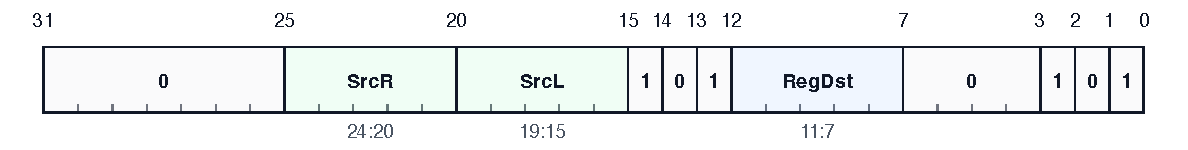
\includegraphics[width=\textwidth]{figs/encoding/scalar_instruction_entries/enc_srl.pdf}\par\smallskip
\begin{description}[leftmargin=0.18\linewidth,style=nextline]
\item[Format] \texttt{L32} \texttt{32-bit} scalar word.
\item[Pattern] \texttt{0000000..........101.....0000101}.
\end{description}
\noindent\textbf{Classification.}\par
\begin{description}[leftmargin=0.18\linewidth,style=nextline]
\item[Category] Integer ALU and Bit-Manipulation.
\item[Family] Arithmetic Operation 64bit.
\item[Execution class] \texttt{ALU}; uop\_kind=ALU.
\end{description}
\noindent\textbf{Operand fields.}\par
\begin{description}[leftmargin=0.18\linewidth,style=nextline]
\item[\texttt{RegDst}] Bits \texttt{11:7 (5b)}. 5-bit scalar destination register written by this instruction; X0 is hardwired to zero, so writes to X0 are ignored.
\item[\texttt{SrcL}] Bits \texttt{19:15 (5b)}. 5-bit scalar source register used as the left input operand.
\item[\texttt{SrcR}] Bits \texttt{24:20 (5b)}. 5-bit scalar source register used as the right input operand before any encoded modifier or shift is applied.
\end{description}
\noindent\textbf{Operation.}\par
\begin{lstlisting}[style=ptoscalarcode]
a = Read(SrcL)
sh = Read(SrcR) & 63
result = a >> sh
Write(RegDst, result)
\end{lstlisting}
\Needspace{0.08\textheight}

\medskip
% Scalar instruction entry source: tools/generate_scalar_instruction_catalog.py.
\subsection{\texttt{SRLI}}
\label{sec:scalar-srli}
\index{SRLI@\texttt{SRLI}}
\begin{sloppypar}\noindent\textbf{Purpose.} Logical right shift (immediate).\end{sloppypar}\smallskip
\noindent\textbf{Syntax.}\par
\begin{lstlisting}[style=ptoscalarcode]
srli SrcL, shamt, ->RegDst
\end{lstlisting}
\noindent\textbf{Encoding.}\par
\noindent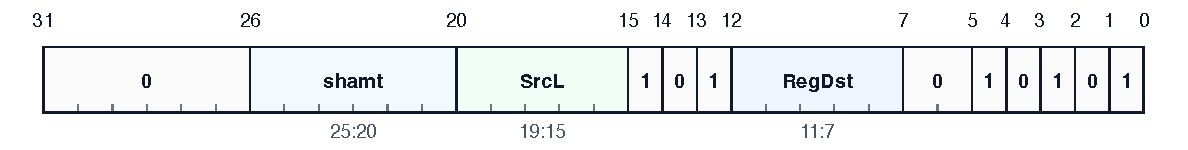
\includegraphics[width=\textwidth]{figs/encoding/scalar_instruction_entries/enc_srli.pdf}\par\smallskip
\begin{description}[leftmargin=0.18\linewidth,style=nextline]
\item[Format] \texttt{L32} \texttt{32-bit} scalar word.
\item[Pattern] \texttt{000000...........101.....0010101}.
\end{description}
\noindent\textbf{Classification.}\par
\begin{description}[leftmargin=0.18\linewidth,style=nextline]
\item[Category] Integer ALU and Bit-Manipulation.
\item[Family] Arithmetic Operation 64bit.
\item[Execution class] \texttt{ALU}; uop\_kind=ALU.
\end{description}
\noindent\textbf{Operand fields.}\par
\begin{description}[leftmargin=0.18\linewidth,style=nextline]
\item[\texttt{RegDst}] Bits \texttt{11:7 (5b)}. 5-bit scalar destination register written by this instruction; X0 is hardwired to zero, so writes to X0 are ignored.
\item[\texttt{SrcL}] Bits \texttt{19:15 (5b)}. 5-bit scalar source register used as the left input operand.
\item[\texttt{shamt}] Bits \texttt{25:20 (6b)}. 6-bit shift amount applied to the modified right operand before the ALU or address calculation uses it.
\end{description}
\noindent\textbf{Operation.}\par
\begin{lstlisting}[style=ptoscalarcode]
a = Read(SrcL)
sh = shamt
result = a >> sh
Write(RegDst, result)
\end{lstlisting}
\Needspace{0.08\textheight}

\medskip
% Scalar instruction entry source: tools/generate_scalar_instruction_catalog.py.
\subsection{\texttt{SRLIW}}
\label{sec:scalar-srliw}
\index{SRLIW@\texttt{SRLIW}}
\begin{sloppypar}\noindent\textbf{Purpose.} Word (32-bit) logical right shift (immediate).\end{sloppypar}\smallskip
\noindent\textbf{Syntax.}\par
\begin{lstlisting}[style=ptoscalarcode]
srliw SrcL, shamt, ->RegDst
\end{lstlisting}
\noindent\textbf{Encoding.}\par
\noindent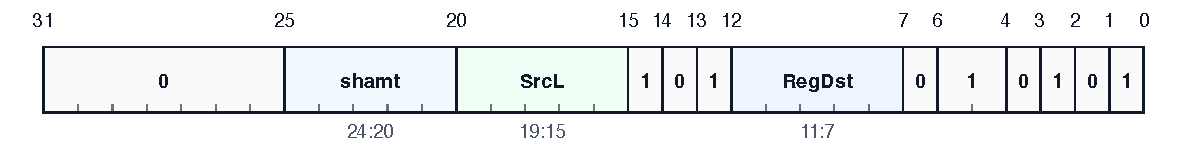
\includegraphics[width=\textwidth]{figs/encoding/scalar_instruction_entries/enc_srliw.pdf}\par\smallskip
\begin{description}[leftmargin=0.18\linewidth,style=nextline]
\item[Format] \texttt{L32} \texttt{32-bit} scalar word.
\item[Pattern] \texttt{0000000..........101.....0110101}.
\end{description}
\noindent\textbf{Classification.}\par
\begin{description}[leftmargin=0.18\linewidth,style=nextline]
\item[Category] Integer ALU and Bit-Manipulation.
\item[Family] Arithmetic Operation 32bit.
\item[Execution class] \texttt{ALU}; uop\_kind=ALU.
\end{description}
\noindent\textbf{Operand fields.}\par
\begin{description}[leftmargin=0.18\linewidth,style=nextline]
\item[\texttt{RegDst}] Bits \texttt{11:7 (5b)}. 5-bit scalar destination register written by this instruction; X0 is hardwired to zero, so writes to X0 are ignored.
\item[\texttt{SrcL}] Bits \texttt{19:15 (5b)}. 5-bit scalar source register used as the left input operand.
\item[\texttt{shamt}] Bits \texttt{24:20 (5b)}. 5-bit shift amount applied to the modified right operand before the ALU or address calculation uses it.
\end{description}
\noindent\textbf{Operation.}\par
\begin{lstlisting}[style=ptoscalarcode]
a = Read(SrcL)[31:0]
sh = shamt
result32 = a >> sh
result = SignExtend32(result32)
Write(RegDst, result)
\end{lstlisting}
\Needspace{0.08\textheight}

\medskip
\input{scalar-instructions/entries/206_srlw.tex}
\medskip
\input{scalar-instructions/entries/210_sub.tex}
\medskip
% Scalar instruction entry source: tools/generate_scalar_instruction_catalog.py.
\subsection{\texttt{SUBI}}
\label{sec:scalar-subi}
\index{SUBI@\texttt{SUBI}}
\begin{sloppypar}\noindent\textbf{Purpose.} Integer subtract-immediate.\end{sloppypar}\smallskip
\noindent\textbf{Syntax.}\par
\begin{lstlisting}[style=ptoscalarcode]
subi SrcL, uimm, ->RegDst
\end{lstlisting}
\noindent\textbf{Encoding.}\par
\noindent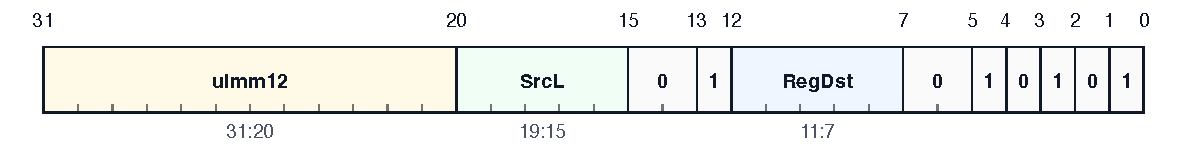
\includegraphics[width=\textwidth]{figs/encoding/scalar_instruction_entries/enc_subi.pdf}\par\smallskip
\begin{description}[leftmargin=0.18\linewidth,style=nextline]
\item[Format] \texttt{L32} \texttt{32-bit} scalar word.
\item[Pattern] \texttt{.................001.....0010101}.
\end{description}
\noindent\textbf{Classification.}\par
\begin{description}[leftmargin=0.18\linewidth,style=nextline]
\item[Category] Integer ALU and Bit-Manipulation.
\item[Family] Arithmetic Operation 64bit.
\item[Execution class] \texttt{ALU}; uop\_kind=ALU.
\end{description}
\noindent\textbf{Operand fields.}\par
\begin{description}[leftmargin=0.18\linewidth,style=nextline]
\item[\texttt{RegDst}] Bits \texttt{11:7 (5b)}. 5-bit scalar destination register written by this instruction; X0 is hardwired to zero, so writes to X0 are ignored.
\item[\texttt{SrcL}] Bits \texttt{19:15 (5b)}. 5-bit scalar source register used as the left input operand.
\item[\texttt{uimm12}] Bits \texttt{31:20 (12b)}. 12-bit unsigned immediate operand consumed directly by the operation.
\end{description}
\noindent\textbf{Operation.}\par
\begin{lstlisting}[style=ptoscalarcode]
lhs = Read(SrcL)
rhs = imm  // immediate as encoded
result = lhs - rhs
Write(RegDst, result)
\end{lstlisting}
\Needspace{0.08\textheight}

\medskip
\input{scalar-instructions/entries/212_subiw.tex}
\medskip
\input{scalar-instructions/entries/213_subw.tex}
\medskip
\input{scalar-instructions/entries/236_xor.tex}
\medskip
\input{scalar-instructions/entries/237_xori.tex}
\medskip
\input{scalar-instructions/entries/238_xoriw.tex}
\medskip
\input{scalar-instructions/entries/239_xorw.tex}
\medskip

\section{Branch, Compare, and PC Control}
Branch and compare instructions update control flow or materialize integer condition results using the scalar register file and PC state.\par\smallskip
{\scriptsize
\begin{longtable}{@{}L{0.24\linewidth}R{0.09\linewidth}L{0.56\linewidth}@{}}
\toprule
Family & Count & Representative instructions \\
\midrule
Branch & 10 & \texttt{B.EQ, B.GE, B.GEU, B.LT, B.LTU, B.NE, B.NZ, B.Z} \\
Compare Instruction & 16 & \texttt{CMP.AND, CMP.ANDI, CMP.EQ, CMP.EQI, CMP.GE, CMP.GEI, CMP.GEU, CMP.GEUI} \\
PC-Relative & 2 & \texttt{ADDTPC, JAL} \\
\bottomrule
\end{longtable}
}

% Scalar instruction entry source: tools/generate_scalar_instruction_catalog.py.
\subsection{\texttt{ADDTPC}}
\label{sec:scalar-addtpc}
\index{ADDTPC@\texttt{ADDTPC}}
\begin{sloppypar}\noindent\textbf{Purpose.} PC-relative addition (adds to the current PC/TPC).\end{sloppypar}\smallskip
\noindent\textbf{Syntax.}\par
\begin{lstlisting}[style=ptoscalarcode]
addtpc simm, ->RegDst
\end{lstlisting}
\noindent\textbf{Encoding.}\par
\noindent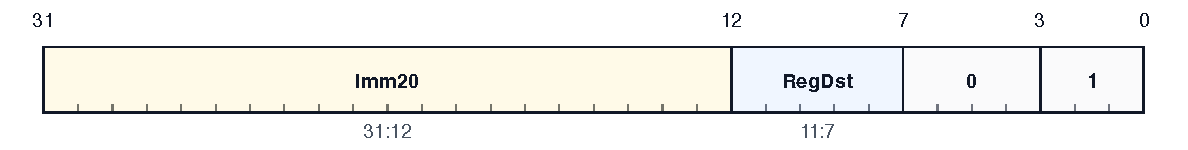
\includegraphics[width=\textwidth]{figs/encoding/scalar_instruction_entries/enc_addtpc.pdf}\par\smallskip
\begin{description}[leftmargin=0.18\linewidth,style=nextline]
\item[Format] \texttt{L32} \texttt{32-bit} scalar word.
\item[Pattern] \texttt{.........................0000111}.
\end{description}
\noindent\textbf{Classification.}\par
\begin{description}[leftmargin=0.18\linewidth,style=nextline]
\item[Category] Branch, Compare, and PC Control.
\item[Family] PC-Relative.
\item[Execution class] \texttt{BRU}; uop\_kind=BRU.
\end{description}
\noindent\textbf{Operand fields.}\par
\begin{description}[leftmargin=0.18\linewidth,style=nextline]
\item[\texttt{RegDst}] Bits \texttt{11:7 (5b)}. 5-bit scalar destination register written by this instruction; X0 is hardwired to zero, so writes to X0 are ignored.
\item[\texttt{imm20}] Bits \texttt{31:12 (20b)}. 20-bit unsigned immediate operand consumed directly by the operation.
\end{description}
\noindent\textbf{Operation.}\par
\begin{lstlisting}[style=ptoscalarcode]
base = CurrentPC()
off = (SignExtend(imm20) << 1)
Write(RegDst, base + off)
\end{lstlisting}
\Needspace{0.08\textheight}

\medskip
\input{scalar-instructions/entries/013_b_eq.tex}
\medskip
% Scalar instruction entry source: tools/generate_scalar_instruction_catalog.py.
\subsection{\texttt{B.GE}}
\label{sec:scalar-b_ge}
\index{B.GE@\texttt{B.GE}}
\begin{sloppypar}\noindent\textbf{Purpose.} Conditional branch. The branch is taken when the selected condition holds (greater-or-equal (signed)).\end{sloppypar}\smallskip
\noindent\textbf{Syntax.}\par
\begin{lstlisting}[style=ptoscalarcode]
b.ge SrcL, SrcR, label
\end{lstlisting}
\noindent\textbf{Encoding.}\par
\noindent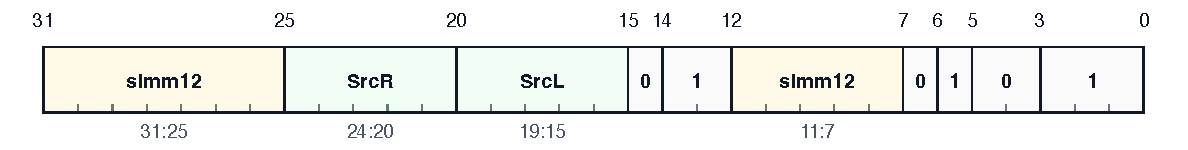
\includegraphics[width=\textwidth]{figs/encoding/scalar_instruction_entries/enc_b_ge.pdf}\par\smallskip
\begin{description}[leftmargin=0.18\linewidth,style=nextline]
\item[Format] \texttt{L32} \texttt{32-bit} scalar word.
\item[Pattern] \texttt{.................011.....0100111}.
\end{description}
\noindent\textbf{Classification.}\par
\begin{description}[leftmargin=0.18\linewidth,style=nextline]
\item[Category] Branch, Compare, and PC Control.
\item[Family] Branch.
\item[Execution class] \texttt{BRU}; uop\_kind=BRU.
\end{description}
\noindent\textbf{Operand fields.}\par
\begin{description}[leftmargin=0.18\linewidth,style=nextline]
\item[\texttt{SrcL}] Bits \texttt{19:15 (5b)}. 5-bit scalar source register used as the left operand of the branch condition.
\item[\texttt{SrcR}] Bits \texttt{24:20 (5b)}. 5-bit scalar source register used as the right operand of the branch condition.
\item[\texttt{simm12}] Bits \texttt{31:25 (7b), 11:7 (5b)}. 12-bit signed PC-relative branch displacement. The decoded offset is sign-extended and added to the current PC when the condition is true. The immediate is split across non-contiguous encoding slices and reassembled before use.
\end{description}
\noindent\textbf{Operation.}\par
\begin{lstlisting}[style=ptoscalarcode]
if (Read(SrcL) >= Read(SrcR)  // signed):
  TPC = <target>
\end{lstlisting}
\Needspace{0.08\textheight}

\medskip
\input{scalar-instructions/entries/015_b_geu.tex}
\medskip
\input{scalar-instructions/entries/016_b_lt.tex}
\medskip
\input{scalar-instructions/entries/017_b_ltu.tex}
\medskip
\input{scalar-instructions/entries/018_b_ne.tex}
\medskip
% Scalar instruction entry source: tools/generate_scalar_instruction_catalog.py.
\subsection{\texttt{B.NZ}}
\label{sec:scalar-b_nz}
\index{B.NZ@\texttt{B.NZ}}
\begin{sloppypar}\noindent\textbf{Purpose.} Conditional branch. The branch is taken when the selected condition holds (non-zero).\end{sloppypar}\smallskip
\noindent\textbf{Syntax.}\par
\begin{lstlisting}[style=ptoscalarcode]
b.nz label
\end{lstlisting}
\noindent\textbf{Encoding.}\par
\noindent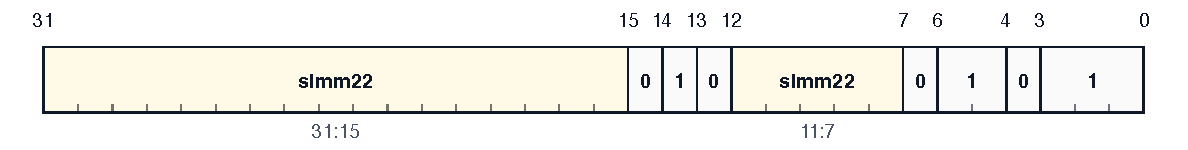
\includegraphics[width=\textwidth]{figs/encoding/scalar_instruction_entries/enc_b_nz.pdf}\par\smallskip
\begin{description}[leftmargin=0.18\linewidth,style=nextline]
\item[Format] \texttt{L32} \texttt{32-bit} scalar word.
\item[Pattern] \texttt{.................010.....0110111}.
\end{description}
\noindent\textbf{Classification.}\par
\begin{description}[leftmargin=0.18\linewidth,style=nextline]
\item[Category] Branch, Compare, and PC Control.
\item[Family] Branch.
\item[Execution class] \texttt{BRU}; uop\_kind=BRU.
\end{description}
\noindent\textbf{Operand fields.}\par
\begin{description}[leftmargin=0.18\linewidth,style=nextline]
\item[\texttt{simm22}] Bits \texttt{31:15 (17b), 11:7 (5b)}. 22-bit signed PC-relative branch displacement. The decoded offset is sign-extended and added to the current PC when the condition is true. The immediate is split across non-contiguous encoding slices and reassembled before use.
\end{description}
\noindent\textbf{Operation.}\par
\begin{lstlisting}[style=ptoscalarcode]
if (branch condition holds (non-zero)):
  TPC = <target>
\end{lstlisting}
\Needspace{0.08\textheight}

\medskip
\input{scalar-instructions/entries/020_b_z.tex}
\medskip
\input{scalar-instructions/entries/033_cmp_and.tex}
\medskip
\input{scalar-instructions/entries/034_cmp_andi.tex}
\medskip
% Scalar instruction entry source: tools/generate_scalar_instruction_catalog.py.
\subsection{\texttt{CMP.EQ}}
\label{sec:scalar-cmp_eq}
\index{CMP.EQ@\texttt{CMP.EQ}}
\begin{sloppypar}\noindent\textbf{Purpose.} Compares SrcL and the modified SrcR for equality and writes 1 or 0 to RegDst.\end{sloppypar}\smallskip
\noindent\textbf{Syntax.}\par
\begin{lstlisting}[style=ptoscalarcode]
cmp.eq SrcL, SrcR<{.sw, .uw}>, ->RegDst
\end{lstlisting}
\noindent\textbf{Encoding.}\par
\noindent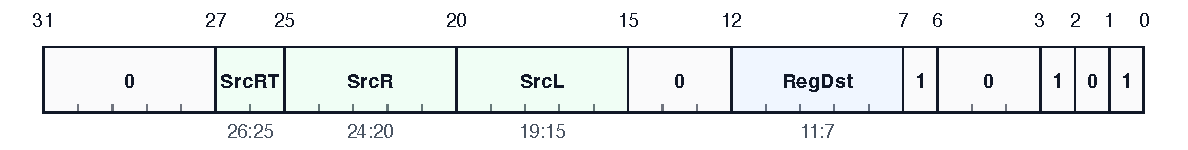
\includegraphics[width=\textwidth]{figs/encoding/scalar_instruction_entries/enc_cmp_eq.pdf}\par\smallskip
\begin{description}[leftmargin=0.18\linewidth,style=nextline]
\item[Format] \texttt{L32} \texttt{32-bit} scalar word.
\item[Pattern] \texttt{00000............000.....1000101}.
\end{description}
\noindent\textbf{Classification.}\par
\begin{description}[leftmargin=0.18\linewidth,style=nextline]
\item[Category] Branch, Compare, and PC Control.
\item[Family] Compare Instruction.
\item[Execution class] \texttt{BRU}; uop\_kind=BRU, bru\_kind=CMP.
\end{description}
\noindent\textbf{Operand fields.}\par
\begin{description}[leftmargin=0.18\linewidth,style=nextline]
\item[\texttt{RegDst}] Bits \texttt{11:7 (5b)}. 5-bit scalar destination register that receives the boolean compare result, encoded as 1 for true and 0 for false; X0 discards the write.
\item[\texttt{SrcL}] Bits \texttt{19:15 (5b)}. 5-bit scalar source register used as the left operand of the comparison.
\item[\texttt{SrcR}] Bits \texttt{24:20 (5b)}. 5-bit scalar source register used as the right operand of the comparison before any SrcRType modifier is applied.
\item[\texttt{SrcRType}] Bits \texttt{26:25 (2b)}. 2-bit modifier for SrcR. It selects the encoded source form shown in the syntax, such as signed-word, unsigned-word, negated, or unmodified register input.
\end{description}
\noindent\textbf{Operation.}\par
\begin{lstlisting}[style=ptoscalarcode]
result = (Read(SrcL) == Read(SrcR)) ? 1 : 0
Write(RegDst, result)
\end{lstlisting}
\Needspace{0.08\textheight}

\medskip
\input{scalar-instructions/entries/036_cmp_eqi.tex}
\medskip
\input{scalar-instructions/entries/037_cmp_ge.tex}
\medskip
\input{scalar-instructions/entries/038_cmp_gei.tex}
\medskip
\input{scalar-instructions/entries/039_cmp_geu.tex}
\medskip
% Scalar instruction entry source: tools/generate_scalar_instruction_catalog.py.
\subsection{\texttt{CMP.GEUI}}
\label{sec:scalar-cmp_geui}
\index{CMP.GEUI@\texttt{CMP.GEUI}}
\begin{sloppypar}\noindent\textbf{Purpose.} Performs an unsigned greater-than-or-equal comparison between SrcL and the immediate operand and writes 1 or 0 to RegDst.\end{sloppypar}\smallskip
\noindent\textbf{Syntax.}\par
\begin{lstlisting}[style=ptoscalarcode]
cmp.geui SrcL, uimm, ->RegDst
\end{lstlisting}
\noindent\textbf{Encoding.}\par
\noindent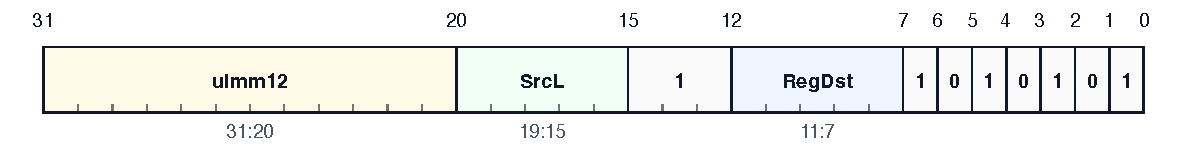
\includegraphics[width=\textwidth]{figs/encoding/scalar_instruction_entries/enc_cmp_geui.pdf}\par\smallskip
\begin{description}[leftmargin=0.18\linewidth,style=nextline]
\item[Format] \texttt{L32} \texttt{32-bit} scalar word.
\item[Pattern] \texttt{.................111.....1010101}.
\end{description}
\noindent\textbf{Classification.}\par
\begin{description}[leftmargin=0.18\linewidth,style=nextline]
\item[Category] Branch, Compare, and PC Control.
\item[Family] Compare Instruction.
\item[Execution class] \texttt{BRU}; uop\_kind=BRU, bru\_kind=CMP.
\end{description}
\noindent\textbf{Operand fields.}\par
\begin{description}[leftmargin=0.18\linewidth,style=nextline]
\item[\texttt{RegDst}] Bits \texttt{11:7 (5b)}. 5-bit scalar destination register that receives the boolean compare result, encoded as 1 for true and 0 for false; X0 discards the write.
\item[\texttt{SrcL}] Bits \texttt{19:15 (5b)}. 5-bit scalar source register used as the left operand of the comparison.
\item[\texttt{uimm12}] Bits \texttt{31:20 (12b)}. 12-bit unsigned immediate operand consumed directly by the operation.
\end{description}
\noindent\textbf{Operation.}\par
\begin{lstlisting}[style=ptoscalarcode]
imm = ZeroExtend(uimm)
result = (Read(SrcL) >= imm  // unsigned) ? 1 : 0
Write(RegDst, result)
\end{lstlisting}
\Needspace{0.08\textheight}

\medskip
% Scalar instruction entry source: tools/generate_scalar_instruction_catalog.py.
\subsection{\texttt{CMP.LT}}
\label{sec:scalar-cmp_lt}
\index{CMP.LT@\texttt{CMP.LT}}
\begin{sloppypar}\noindent\textbf{Purpose.} Performs a signed less-than comparison between SrcL and SrcR and writes 1 or 0 to RegDst.\end{sloppypar}\smallskip
\noindent\textbf{Syntax.}\par
\begin{lstlisting}[style=ptoscalarcode]
cmp.lt SrcL, SrcR<{.sw, .uw}>, ->RegDst
\end{lstlisting}
\noindent\textbf{Encoding.}\par
\noindent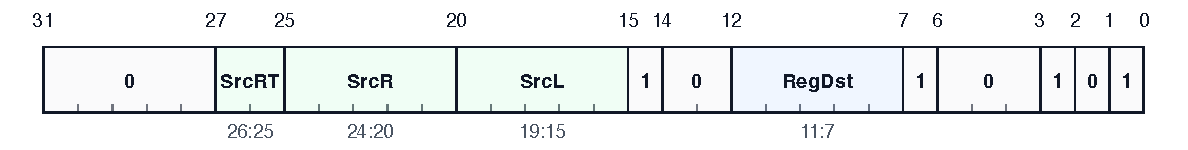
\includegraphics[width=\textwidth]{figs/encoding/scalar_instruction_entries/enc_cmp_lt.pdf}\par\smallskip
\begin{description}[leftmargin=0.18\linewidth,style=nextline]
\item[Format] \texttt{L32} \texttt{32-bit} scalar word.
\item[Pattern] \texttt{00000............100.....1000101}.
\end{description}
\noindent\textbf{Classification.}\par
\begin{description}[leftmargin=0.18\linewidth,style=nextline]
\item[Category] Branch, Compare, and PC Control.
\item[Family] Compare Instruction.
\item[Execution class] \texttt{BRU}; uop\_kind=BRU, bru\_kind=CMP.
\end{description}
\noindent\textbf{Operand fields.}\par
\begin{description}[leftmargin=0.18\linewidth,style=nextline]
\item[\texttt{RegDst}] Bits \texttt{11:7 (5b)}. 5-bit scalar destination register that receives the boolean compare result, encoded as 1 for true and 0 for false; X0 discards the write.
\item[\texttt{SrcL}] Bits \texttt{19:15 (5b)}. 5-bit scalar source register used as the left operand of the comparison.
\item[\texttt{SrcR}] Bits \texttt{24:20 (5b)}. 5-bit scalar source register used as the right operand of the comparison before any SrcRType modifier is applied.
\item[\texttt{SrcRType}] Bits \texttt{26:25 (2b)}. 2-bit modifier for SrcR. It selects the encoded source form shown in the syntax, such as signed-word, unsigned-word, negated, or unmodified register input.
\end{description}
\noindent\textbf{Operation.}\par
\begin{lstlisting}[style=ptoscalarcode]
result = (Read(SrcL) < Read(SrcR)  // signed) ? 1 : 0
Write(RegDst, result)
\end{lstlisting}
\Needspace{0.08\textheight}

\medskip
% Scalar instruction entry source: tools/generate_scalar_instruction_catalog.py.
\subsection{\texttt{CMP.LTI}}
\label{sec:scalar-cmp_lti}
\index{CMP.LTI@\texttt{CMP.LTI}}
\begin{sloppypar}\noindent\textbf{Purpose.} Performs a signed less-than comparison between SrcL and the immediate operand and writes 1 or 0 to RegDst.\end{sloppypar}\smallskip
\noindent\textbf{Syntax.}\par
\begin{lstlisting}[style=ptoscalarcode]
cmp.lti SrcL, simm, ->RegDst
\end{lstlisting}
\noindent\textbf{Encoding.}\par
\noindent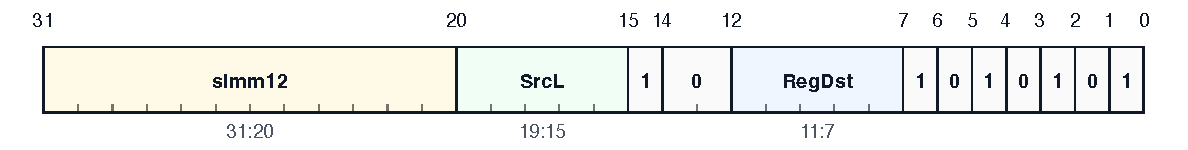
\includegraphics[width=\textwidth]{figs/encoding/scalar_instruction_entries/enc_cmp_lti.pdf}\par\smallskip
\begin{description}[leftmargin=0.18\linewidth,style=nextline]
\item[Format] \texttt{L32} \texttt{32-bit} scalar word.
\item[Pattern] \texttt{.................100.....1010101}.
\end{description}
\noindent\textbf{Classification.}\par
\begin{description}[leftmargin=0.18\linewidth,style=nextline]
\item[Category] Branch, Compare, and PC Control.
\item[Family] Compare Instruction.
\item[Execution class] \texttt{BRU}; uop\_kind=BRU, bru\_kind=CMP.
\end{description}
\noindent\textbf{Operand fields.}\par
\begin{description}[leftmargin=0.18\linewidth,style=nextline]
\item[\texttt{RegDst}] Bits \texttt{11:7 (5b)}. 5-bit scalar destination register that receives the boolean compare result, encoded as 1 for true and 0 for false; X0 discards the write.
\item[\texttt{SrcL}] Bits \texttt{19:15 (5b)}. 5-bit scalar source register used as the left operand of the comparison.
\item[\texttt{simm12}] Bits \texttt{31:20 (12b)}. 12-bit signed immediate operand that is sign-extended before use.
\end{description}
\noindent\textbf{Operation.}\par
\begin{lstlisting}[style=ptoscalarcode]
imm = SignExtend(simm)
result = (Read(SrcL) < imm  // signed) ? 1 : 0
Write(RegDst, result)
\end{lstlisting}
\Needspace{0.08\textheight}

\medskip
\input{scalar-instructions/entries/043_cmp_ltu.tex}
\medskip
\input{scalar-instructions/entries/044_cmp_ltui.tex}
\medskip
\input{scalar-instructions/entries/045_cmp_ne.tex}
\medskip
% Scalar instruction entry source: tools/generate_scalar_instruction_catalog.py.
\subsection{\texttt{CMP.NEI}}
\label{sec:scalar-cmp_nei}
\index{CMP.NEI@\texttt{CMP.NEI}}
\begin{sloppypar}\noindent\textbf{Purpose.} Compares SrcL and the immediate operand for inequality and writes 1 or 0 to RegDst.\end{sloppypar}\smallskip
\noindent\textbf{Syntax.}\par
\begin{lstlisting}[style=ptoscalarcode]
cmp.nei SrcL, simm, ->RegDst
\end{lstlisting}
\noindent\textbf{Encoding.}\par
\noindent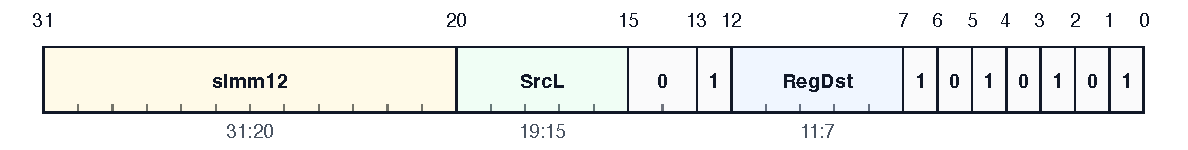
\includegraphics[width=\textwidth]{figs/encoding/scalar_instruction_entries/enc_cmp_nei.pdf}\par\smallskip
\begin{description}[leftmargin=0.18\linewidth,style=nextline]
\item[Format] \texttt{L32} \texttt{32-bit} scalar word.
\item[Pattern] \texttt{.................001.....1010101}.
\end{description}
\noindent\textbf{Classification.}\par
\begin{description}[leftmargin=0.18\linewidth,style=nextline]
\item[Category] Branch, Compare, and PC Control.
\item[Family] Compare Instruction.
\item[Execution class] \texttt{BRU}; uop\_kind=BRU, bru\_kind=CMP.
\end{description}
\noindent\textbf{Operand fields.}\par
\begin{description}[leftmargin=0.18\linewidth,style=nextline]
\item[\texttt{RegDst}] Bits \texttt{11:7 (5b)}. 5-bit scalar destination register that receives the boolean compare result, encoded as 1 for true and 0 for false; X0 discards the write.
\item[\texttt{SrcL}] Bits \texttt{19:15 (5b)}. 5-bit scalar source register used as the left operand of the comparison.
\item[\texttt{simm12}] Bits \texttt{31:20 (12b)}. 12-bit signed immediate operand that is sign-extended before use.
\end{description}
\noindent\textbf{Operation.}\par
\begin{lstlisting}[style=ptoscalarcode]
imm = SignExtend(simm)
result = (Read(SrcL) != imm) ? 1 : 0
Write(RegDst, result)
\end{lstlisting}
\Needspace{0.08\textheight}

\medskip
\input{scalar-instructions/entries/047_cmp_or.tex}
\medskip
% Scalar instruction entry source: tools/generate_scalar_instruction_catalog.py.
\subsection{\texttt{CMP.ORI}}
\label{sec:scalar-cmp_ori}
\index{CMP.ORI@\texttt{CMP.ORI}}
\begin{sloppypar}\noindent\textbf{Purpose.} Tests whether the bitwise OR of SrcL and the immediate operand is nonzero, then writes 1 or 0 to RegDst.\end{sloppypar}\smallskip
\noindent\textbf{Syntax.}\par
\begin{lstlisting}[style=ptoscalarcode]
cmp.ori SrcL, simm, ->RegDst
\end{lstlisting}
\noindent\textbf{Encoding.}\par
\noindent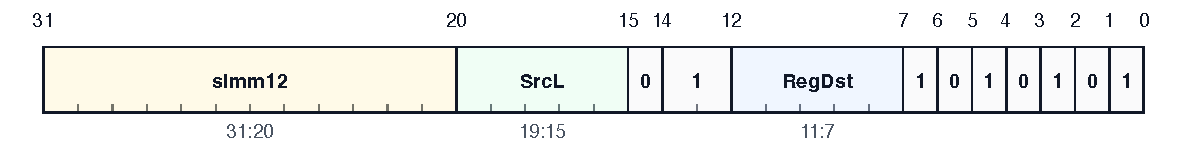
\includegraphics[width=\textwidth]{figs/encoding/scalar_instruction_entries/enc_cmp_ori.pdf}\par\smallskip
\begin{description}[leftmargin=0.18\linewidth,style=nextline]
\item[Format] \texttt{L32} \texttt{32-bit} scalar word.
\item[Pattern] \texttt{.................011.....1010101}.
\end{description}
\noindent\textbf{Classification.}\par
\begin{description}[leftmargin=0.18\linewidth,style=nextline]
\item[Category] Branch, Compare, and PC Control.
\item[Family] Compare Instruction.
\item[Execution class] \texttt{BRU}; uop\_kind=BRU, bru\_kind=CMP.
\end{description}
\noindent\textbf{Operand fields.}\par
\begin{description}[leftmargin=0.18\linewidth,style=nextline]
\item[\texttt{RegDst}] Bits \texttt{11:7 (5b)}. 5-bit scalar destination register that receives the boolean compare result, encoded as 1 for true and 0 for false; X0 discards the write.
\item[\texttt{SrcL}] Bits \texttt{19:15 (5b)}. 5-bit scalar source register used as the left operand of the comparison.
\item[\texttt{simm12}] Bits \texttt{31:20 (12b)}. 12-bit signed immediate operand that is sign-extended before use.
\end{description}
\noindent\textbf{Operation.}\par
\begin{lstlisting}[style=ptoscalarcode]
lhs = Read(SrcL)
imm = SignExtend(simm)
result = ((lhs | imm) != 0) ? 1 : 0
Write(RegDst, result)
\end{lstlisting}
\Needspace{0.08\textheight}

\medskip
\input{scalar-instructions/entries/096_j.tex}
\medskip
% Scalar instruction entry source: tools/generate_scalar_instruction_catalog.py.
\subsection{\texttt{JR}}
\label{sec:scalar-jr}
\index{JR@\texttt{JR}}
\begin{sloppypar}\noindent\textbf{Purpose.} Jump to an address formed from a base register plus an immediate offset.\end{sloppypar}\smallskip
\noindent\textbf{Syntax.}\par
\begin{lstlisting}[style=ptoscalarcode]
jr SrcL, label
\end{lstlisting}
\noindent\textbf{Encoding.}\par
\noindent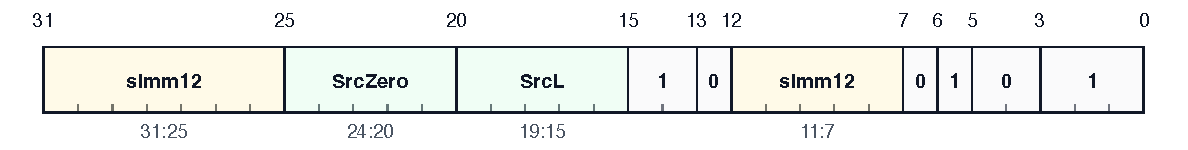
\includegraphics[width=\textwidth]{figs/encoding/scalar_instruction_entries/enc_jr.pdf}\par\smallskip
\begin{description}[leftmargin=0.18\linewidth,style=nextline]
\item[Format] \texttt{L32} \texttt{32-bit} scalar word.
\item[Pattern] \texttt{.................110.....0100111}.
\end{description}
\noindent\textbf{Classification.}\par
\begin{description}[leftmargin=0.18\linewidth,style=nextline]
\item[Category] Branch, Compare, and PC Control.
\item[Family] Branch.
\item[Execution class] \texttt{BRU}; uop\_kind=BRU.
\end{description}
\noindent\textbf{Operand fields.}\par
\begin{description}[leftmargin=0.18\linewidth,style=nextline]
\item[\texttt{SrcL}] Bits \texttt{19:15 (5b)}. 5-bit scalar source register used as the left operand of the branch condition.
\item[\texttt{SrcZero}] Bits \texttt{24:20 (5b)}. 5-bit source-register field that must encode X0; it occupies the standard source slot for encodings that do not consume a second register operand.
\item[\texttt{simm12}] Bits \texttt{31:25 (7b), 11:7 (5b)}. 12-bit signed PC-relative branch displacement. The decoded offset is sign-extended and added to the current PC when the condition is true. The immediate is split across non-contiguous encoding slices and reassembled before use.
\end{description}
\noindent\textbf{Operation.}\par
\begin{lstlisting}[style=ptoscalarcode]
TPC = <target>
\end{lstlisting}
\Needspace{0.08\textheight}

\medskip
% Scalar instruction entry source: tools/generate_scalar_instruction_catalog.py.
\subsection{\texttt{JAL}}
\label{sec:scalar-jal}
\index{JAL@\texttt{JAL}}
\begin{sloppypar}\noindent\textbf{Purpose.} Writes the return address to Ra and transfers control to the PC-relative target.\end{sloppypar}\smallskip
\noindent\textbf{Syntax.}\par
\begin{lstlisting}[style=ptoscalarcode]
jal simm, ->Ra
\end{lstlisting}
\noindent\textbf{Encoding.}\par
\noindent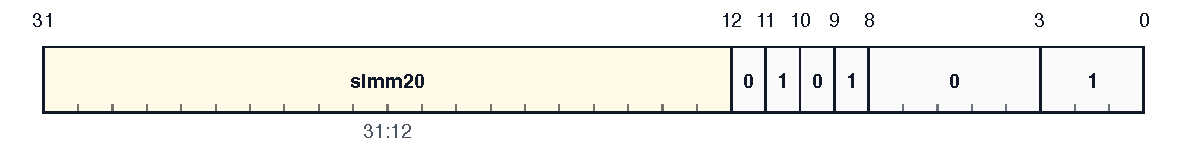
\includegraphics[width=\textwidth]{figs/encoding/scalar_instruction_entries/enc_jal.pdf}\par\smallskip
\begin{description}[leftmargin=0.18\linewidth,style=nextline]
\item[Format] \texttt{L32} \texttt{32-bit} scalar word.
\item[Pattern] \texttt{....................010100000111}.
\end{description}
\noindent\textbf{Classification.}\par
\begin{description}[leftmargin=0.18\linewidth,style=nextline]
\item[Category] Branch, Compare, and PC Control.
\item[Family] PC-Relative.
\item[Execution class] \texttt{BRU}; uop\_kind=BRU.
\end{description}
\noindent\textbf{Operand fields.}\par
\begin{description}[leftmargin=0.18\linewidth,style=nextline]
\item[\texttt{simm20}] Bits \texttt{31:12 (20b)}. 20-bit signed PC-relative displacement used to form the jump or address result.
\end{description}
\noindent\textbf{Operation.}\par
\begin{lstlisting}[style=ptoscalarcode]
base = CurrentPC()
off = (ZeroExtend(imm20) << 1)
ra = base + off
\end{lstlisting}
\Needspace{0.08\textheight}

\medskip

\section{Load, Store, and Address Generation}
Address-generation instructions calculate load/store addresses and perform scalar memory transfers through base-register, immediate, symbol, and unscaled addressing forms.\par\smallskip
{\scriptsize
\begin{longtable}{@{}L{0.24\linewidth}R{0.09\linewidth}L{0.56\linewidth}@{}}
\toprule
Family & Count & Representative instructions \\
\midrule
Load Immediate Offset & 7 & \texttt{LBI, LBUI, LDI, LHI, LHUI, LWI, LWUI} \\
Load Register Offset & 8 & \texttt{LB, LBU, LD, LH, LHU, LW, LWU, PRF} \\
Load Symbol & 7 & \texttt{LB.PCR, LBU.PCR, LD.PCR, LH.PCR, LHU.PCR, LW.PCR, LWU.PCR} \\
Load UnScaled & 6 & \texttt{LDI.U, LHI.U, LHUI.U, LWI.U, LWUI.U, PRFI.U} \\
Store Immediate Offset & 7 & \texttt{SBI, SDI, SDI.U, SHI, SHI.U, SWI, SWI.U} \\
Store Register Offset & 7 & \texttt{SB, SD, SD.U, SH, SH.U, SW, SW.U} \\
Store Symbol & 4 & \texttt{SB.PCR, SD.PCR, SH.PCR, SW.PCR} \\
\bottomrule
\end{longtable}
}

\input{scalar-instructions/entries/098_lb.tex}
\medskip
\input{scalar-instructions/entries/099_lb_pcr.tex}
\medskip
\input{scalar-instructions/entries/100_lbi.tex}
\medskip
\input{scalar-instructions/entries/101_lbu.tex}
\medskip
% Scalar instruction entry source: tools/generate_scalar_instruction_catalog.py.
\subsection{\texttt{LBU.PCR}}
\label{sec:scalar-lbu_pcr}
\index{LBU.PCR@\texttt{LBU.PCR}}
\begin{sloppypar}\noindent\textbf{Purpose.} Loads an unsigned 8-bit value from memory using PC-relative/symbol addressing and writes the result to the selected destination.\end{sloppypar}\smallskip
\noindent\textbf{Syntax.}\par
\begin{lstlisting}[style=ptoscalarcode]
lbu.pcr [symbol], ->RegDst
\end{lstlisting}
\noindent\textbf{Encoding.}\par
\noindent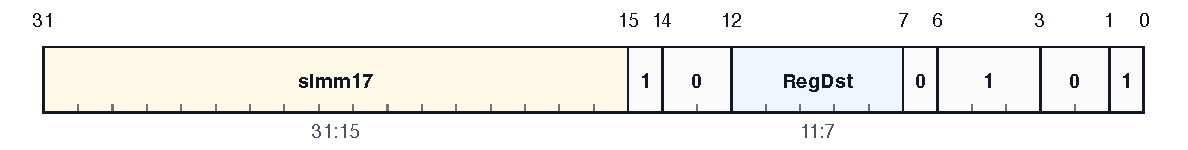
\includegraphics[width=\textwidth]{figs/encoding/scalar_instruction_entries/enc_lbu_pcr.pdf}\par\smallskip
\begin{description}[leftmargin=0.18\linewidth,style=nextline]
\item[Format] \texttt{L32} \texttt{32-bit} scalar word.
\item[Pattern] \texttt{.................100.....0111001}.
\end{description}
\noindent\textbf{Classification.}\par
\begin{description}[leftmargin=0.18\linewidth,style=nextline]
\item[Category] Load, Store, and Address Generation.
\item[Family] Load Symbol.
\item[Execution class] \texttt{LDA}; uop\_kind=AGU, agu\_kind=LDA.
\end{description}
\noindent\textbf{Operand fields.}\par
\begin{description}[leftmargin=0.18\linewidth,style=nextline]
\item[\texttt{RegDst}] Bits \texttt{11:7 (5b)}. 5-bit scalar destination register that receives the loaded value after any sign or zero extension; X0 discards the load result.
\item[\texttt{simm17}] Bits \texttt{31:15 (17b)}. 17-bit signed address displacement added to the base register to form the effective address.
\end{description}
\noindent\textbf{Operation.}\par
\begin{lstlisting}[style=ptoscalarcode]
addr = ComputeAddress(/* per syntax */)
value = Load8(addr)
value = ZeroExtend(value)
Write(RegDst, value)
\end{lstlisting}
\Needspace{0.08\textheight}

\medskip
\input{scalar-instructions/entries/103_lbui.tex}
\medskip
\input{scalar-instructions/entries/104_ld.tex}
\medskip
\input{scalar-instructions/entries/108_ld_pcr.tex}
\medskip
\input{scalar-instructions/entries/114_ldi.tex}
\medskip
\input{scalar-instructions/entries/115_ldi_u.tex}
\medskip
% Scalar instruction entry source: tools/generate_scalar_instruction_catalog.py.
\subsection{\texttt{LH}}
\label{sec:scalar-lh}
\index{LH@\texttt{LH}}
\begin{sloppypar}\noindent\textbf{Purpose.} Loads a signed 16-bit value from memory using register-offset addressing and writes the result to the selected destination.\end{sloppypar}\smallskip
\noindent\textbf{Syntax.}\par
\begin{lstlisting}[style=ptoscalarcode]
lh [SrcL, SrcR<{.sw,.uw,.neg}><<<shamt>], ->RegDst
\end{lstlisting}
\noindent\textbf{Encoding.}\par
\noindent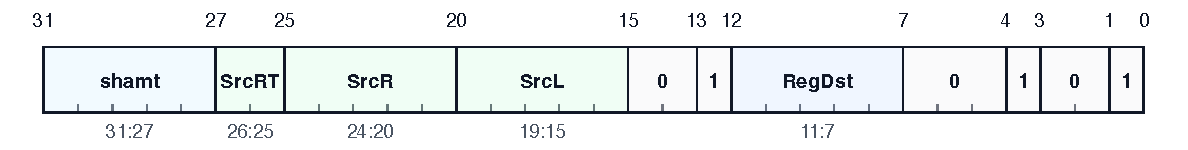
\includegraphics[width=\textwidth]{figs/encoding/scalar_instruction_entries/enc_lh.pdf}\par\smallskip
\begin{description}[leftmargin=0.18\linewidth,style=nextline]
\item[Format] \texttt{L32} \texttt{32-bit} scalar word.
\item[Pattern] \texttt{.................001.....0001001}.
\end{description}
\noindent\textbf{Classification.}\par
\begin{description}[leftmargin=0.18\linewidth,style=nextline]
\item[Category] Load, Store, and Address Generation.
\item[Family] Load Register Offset.
\item[Execution class] \texttt{LDA/BASE\_REG}; uop\_kind=AGU, agu\_kind=LDA, addr\_mode=BASE\_REG.
\end{description}
\noindent\textbf{Operand fields.}\par
\begin{description}[leftmargin=0.18\linewidth,style=nextline]
\item[\texttt{RegDst}] Bits \texttt{11:7 (5b)}. 5-bit scalar destination register that receives the loaded value after any sign or zero extension; X0 discards the load result.
\item[\texttt{SrcL}] Bits \texttt{19:15 (5b)}. 5-bit scalar source register used as the base address for the memory access.
\item[\texttt{SrcR}] Bits \texttt{24:20 (5b)}. 5-bit scalar source register used as the register offset component of the effective address.
\item[\texttt{SrcRType}] Bits \texttt{26:25 (2b)}. 2-bit modifier for SrcR. It selects the encoded source form shown in the syntax, such as signed-word, unsigned-word, negated, or unmodified register input.
\item[\texttt{shamt}] Bits \texttt{31:27 (5b)}. 5-bit shift amount applied to the modified right operand before the ALU or address calculation uses it.
\end{description}
\noindent\textbf{Operation.}\par
\begin{lstlisting}[style=ptoscalarcode]
addr = ComputeAddress(/* per syntax */)
value = Load16(addr)
value = SignExtend(value)
Write(RegDst, value)
\end{lstlisting}
\Needspace{0.08\textheight}

\medskip
\input{scalar-instructions/entries/117_lh_pcr.tex}
\medskip
\input{scalar-instructions/entries/118_lhi.tex}
\medskip
% Scalar instruction entry source: tools/generate_scalar_instruction_catalog.py.
\subsection{\texttt{LHI.U}}
\label{sec:scalar-lhi_u}
\index{LHI.U@\texttt{LHI.U}}
\begin{sloppypar}\noindent\textbf{Purpose.} Loads a signed 16-bit value from memory using unscaled immediate-offset addressing and writes the result to the selected destination.\end{sloppypar}\smallskip
\noindent\textbf{Syntax.}\par
\begin{lstlisting}[style=ptoscalarcode]
lhi.u [SrcL, simm], ->RegDst
\end{lstlisting}
\noindent\textbf{Encoding.}\par
\noindent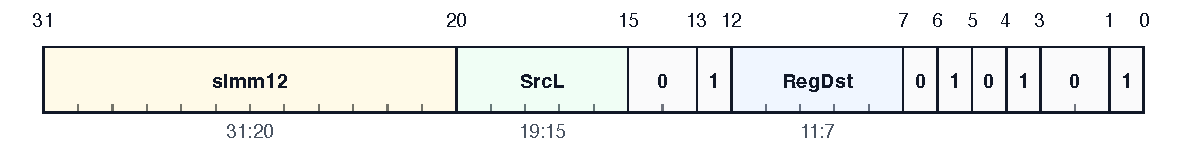
\includegraphics[width=\textwidth]{figs/encoding/scalar_instruction_entries/enc_lhi_u.pdf}\par\smallskip
\begin{description}[leftmargin=0.18\linewidth,style=nextline]
\item[Format] \texttt{L32} \texttt{32-bit} scalar word.
\item[Pattern] \texttt{.................001.....0101001}.
\end{description}
\noindent\textbf{Classification.}\par
\begin{description}[leftmargin=0.18\linewidth,style=nextline]
\item[Category] Load, Store, and Address Generation.
\item[Family] Load UnScaled.
\item[Execution class] \texttt{LDA/UNSCALED}; uop\_kind=AGU, agu\_kind=LDA, addr\_mode=UNSCALED.
\end{description}
\noindent\textbf{Operand fields.}\par
\begin{description}[leftmargin=0.18\linewidth,style=nextline]
\item[\texttt{RegDst}] Bits \texttt{11:7 (5b)}. 5-bit scalar destination register that receives the loaded value after any sign or zero extension; X0 discards the load result.
\item[\texttt{SrcL}] Bits \texttt{19:15 (5b)}. 5-bit scalar source register used as the base address for the memory access.
\item[\texttt{simm12}] Bits \texttt{31:20 (12b)}. 12-bit signed address displacement added to the base register to form the effective address.
\end{description}
\noindent\textbf{Operation.}\par
\begin{lstlisting}[style=ptoscalarcode]
addr = ComputeAddress(/* per syntax */)
value = Load16(addr)
value = SignExtend(value)
Write(RegDst, value)
\end{lstlisting}
\Needspace{0.08\textheight}

\medskip
\input{scalar-instructions/entries/120_lhu.tex}
\medskip
\input{scalar-instructions/entries/121_lhu_pcr.tex}
\medskip
\input{scalar-instructions/entries/122_lhui.tex}
\medskip
\input{scalar-instructions/entries/123_lhui_u.tex}
\medskip
\input{scalar-instructions/entries/130_lw.tex}
\medskip
% Scalar instruction entry source: tools/generate_scalar_instruction_catalog.py.
\subsection{\texttt{LW.PCR}}
\label{sec:scalar-lw_pcr}
\index{LW.PCR@\texttt{LW.PCR}}
\begin{sloppypar}\noindent\textbf{Purpose.} Loads a signed 32-bit value from memory using PC-relative/symbol addressing and writes the result to the selected destination.\end{sloppypar}\smallskip
\noindent\textbf{Syntax.}\par
\begin{lstlisting}[style=ptoscalarcode]
lw.pcr [symbol], ->RegDst
\end{lstlisting}
\noindent\textbf{Encoding.}\par
\noindent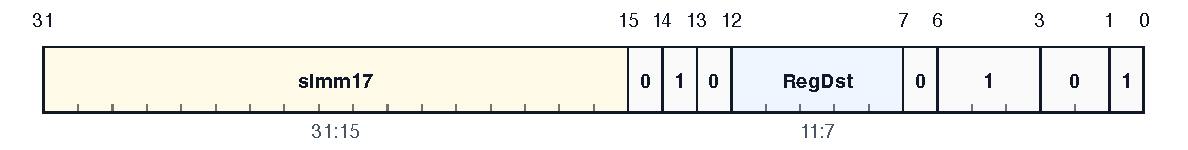
\includegraphics[width=\textwidth]{figs/encoding/scalar_instruction_entries/enc_lw_pcr.pdf}\par\smallskip
\begin{description}[leftmargin=0.18\linewidth,style=nextline]
\item[Format] \texttt{L32} \texttt{32-bit} scalar word.
\item[Pattern] \texttt{.................010.....0111001}.
\end{description}
\noindent\textbf{Classification.}\par
\begin{description}[leftmargin=0.18\linewidth,style=nextline]
\item[Category] Load, Store, and Address Generation.
\item[Family] Load Symbol.
\item[Execution class] \texttt{LDA}; uop\_kind=AGU, agu\_kind=LDA.
\end{description}
\noindent\textbf{Operand fields.}\par
\begin{description}[leftmargin=0.18\linewidth,style=nextline]
\item[\texttt{RegDst}] Bits \texttt{11:7 (5b)}. 5-bit scalar destination register that receives the loaded value after any sign or zero extension; X0 discards the load result.
\item[\texttt{simm17}] Bits \texttt{31:15 (17b)}. 17-bit signed address displacement added to the base register to form the effective address.
\end{description}
\noindent\textbf{Operation.}\par
\begin{lstlisting}[style=ptoscalarcode]
addr = ComputeAddress(/* per syntax */)
value = Load32(addr)
value = SignExtend(value)
Write(RegDst, value)
\end{lstlisting}
\Needspace{0.08\textheight}

\medskip
\input{scalar-instructions/entries/140_lwi.tex}
\medskip
\input{scalar-instructions/entries/141_lwi_u.tex}
\medskip
\input{scalar-instructions/entries/142_lwu.tex}
\medskip
\input{scalar-instructions/entries/143_lwu_pcr.tex}
\medskip
\input{scalar-instructions/entries/144_lwui.tex}
\medskip
\input{scalar-instructions/entries/145_lwui_u.tex}
\medskip
% Scalar instruction entry source: tools/generate_scalar_instruction_catalog.py.
\subsection{\texttt{PRF}}
\label{sec:scalar-prf}
\index{PRF@\texttt{PRF}}
\begin{sloppypar}\noindent\textbf{Purpose.} Issues a prefetch request for the address computed by the selected addressing form.\end{sloppypar}\smallskip
\noindent\textbf{Syntax.}\par
\begin{lstlisting}[style=ptoscalarcode]
prf [SrcL, SrcR<{.sw,.uw,.neg}><<<shamt>]
\end{lstlisting}
\noindent\textbf{Encoding.}\par
\noindent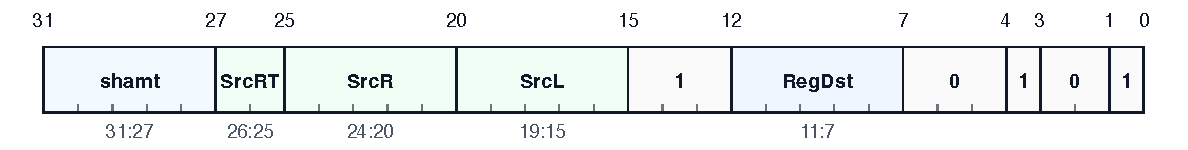
\includegraphics[width=\textwidth]{figs/encoding/scalar_instruction_entries/enc_prf.pdf}\par\smallskip
\begin{description}[leftmargin=0.18\linewidth,style=nextline]
\item[Format] \texttt{L32} \texttt{32-bit} scalar word.
\item[Pattern] \texttt{.................111.....0001001}.
\end{description}
\noindent\textbf{Classification.}\par
\begin{description}[leftmargin=0.18\linewidth,style=nextline]
\item[Category] Load, Store, and Address Generation.
\item[Family] Load Register Offset.
\item[Execution class] \texttt{LDA/BASE\_REG}; uop\_kind=AGU, agu\_kind=LDA, addr\_mode=BASE\_REG.
\end{description}
\noindent\textbf{Operand fields.}\par
\begin{description}[leftmargin=0.18\linewidth,style=nextline]
\item[\texttt{RegDst}] Bits \texttt{11:7 (5b)}. 5-bit scalar destination register that receives the loaded value after any sign or zero extension; X0 discards the load result.
\item[\texttt{SrcL}] Bits \texttt{19:15 (5b)}. 5-bit scalar source register used as the base address for the memory access.
\item[\texttt{SrcR}] Bits \texttt{24:20 (5b)}. 5-bit scalar source register used as the register offset component of the effective address.
\item[\texttt{SrcRType}] Bits \texttt{26:25 (2b)}. 2-bit modifier for SrcR. It selects the encoded source form shown in the syntax, such as signed-word, unsigned-word, negated, or unmodified register input.
\item[\texttt{shamt}] Bits \texttt{31:27 (5b)}. 5-bit shift amount applied to the modified right operand before the ALU or address calculation uses it.
\end{description}
\noindent\textbf{Operation.}\par
\begin{lstlisting}[style=ptoscalarcode]
EA = Read(SrcL) + (ApplySrcRType(SrcRType, Read(SrcR)) << shamt)
PrefetchHint(EA)  // non-faulting
\end{lstlisting}
\Needspace{0.08\textheight}

\medskip
% Scalar instruction entry source: tools/generate_scalar_instruction_catalog.py.
\subsection{\texttt{PRFI.U}}
\label{sec:scalar-prfi_u}
\index{PRFI.U@\texttt{PRFI.U}}
\begin{sloppypar}\noindent\textbf{Purpose.} Issues a prefetch request for the address computed by the selected addressing form.\end{sloppypar}\smallskip
\noindent\textbf{Syntax.}\par
\begin{lstlisting}[style=ptoscalarcode]
prfi.u [SrcL, simm]
\end{lstlisting}
\noindent\textbf{Encoding.}\par
\noindent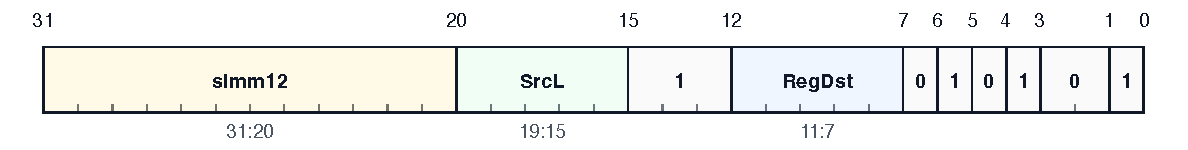
\includegraphics[width=\textwidth]{figs/encoding/scalar_instruction_entries/enc_prfi_u.pdf}\par\smallskip
\begin{description}[leftmargin=0.18\linewidth,style=nextline]
\item[Format] \texttt{L32} \texttt{32-bit} scalar word.
\item[Pattern] \texttt{.................111.....0101001}.
\end{description}
\noindent\textbf{Classification.}\par
\begin{description}[leftmargin=0.18\linewidth,style=nextline]
\item[Category] Load, Store, and Address Generation.
\item[Family] Load UnScaled.
\item[Execution class] \texttt{LDA/UNSCALED}; uop\_kind=AGU, agu\_kind=LDA, addr\_mode=UNSCALED.
\end{description}
\noindent\textbf{Operand fields.}\par
\begin{description}[leftmargin=0.18\linewidth,style=nextline]
\item[\texttt{RegDst}] Bits \texttt{11:7 (5b)}. 5-bit scalar destination register that receives the loaded value after any sign or zero extension; X0 discards the load result.
\item[\texttt{SrcL}] Bits \texttt{19:15 (5b)}. 5-bit scalar source register used as the base address for the memory access.
\item[\texttt{simm12}] Bits \texttt{31:20 (12b)}. 12-bit signed address displacement added to the base register to form the effective address.
\end{description}
\noindent\textbf{Operation.}\par
\begin{lstlisting}[style=ptoscalarcode]
EA = Read(SrcL) + SignExtend(simm12)
PrefetchHint(EA)  // non-faulting
\end{lstlisting}
\Needspace{0.08\textheight}

\medskip
\input{scalar-instructions/entries/167_sb.tex}
\medskip
% Scalar instruction entry source: tools/generate_scalar_instruction_catalog.py.
\subsection{\texttt{SB.PCR}}
\label{sec:scalar-sb_pcr}
\index{SB.PCR@\texttt{SB.PCR}}
\begin{sloppypar}\noindent\textbf{Purpose.} Stores a 8-bit value to memory using PC-relative/symbol addressing.\end{sloppypar}\smallskip
\noindent\textbf{Syntax.}\par
\begin{lstlisting}[style=ptoscalarcode]
sb.pcr SrcL, [symbol]
\end{lstlisting}
\noindent\textbf{Encoding.}\par
\noindent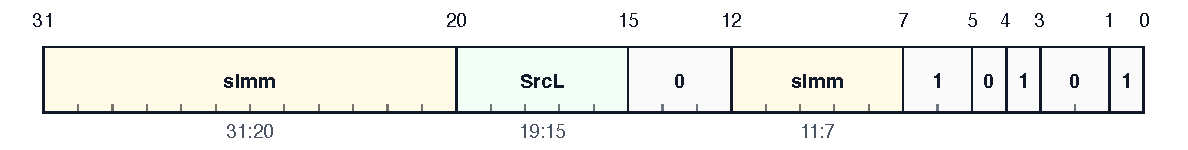
\includegraphics[width=\textwidth]{figs/encoding/scalar_instruction_entries/enc_sb_pcr.pdf}\par\smallskip
\begin{description}[leftmargin=0.18\linewidth,style=nextline]
\item[Format] \texttt{L32} \texttt{32-bit} scalar word.
\item[Pattern] \texttt{.................000.....1101001}.
\end{description}
\noindent\textbf{Classification.}\par
\begin{description}[leftmargin=0.18\linewidth,style=nextline]
\item[Category] Load, Store, and Address Generation.
\item[Family] Store Symbol.
\item[Execution class] \texttt{STA}; uop\_kind=AGU, agu\_kind=STA, split=AGU+STD.
\end{description}
\noindent\textbf{Operand fields.}\par
\begin{description}[leftmargin=0.18\linewidth,style=nextline]
\item[\texttt{SrcL}] Bits \texttt{19:15 (5b)}. 5-bit scalar source register used as the base address for the memory access.
\item[\texttt{simm}] Bits \texttt{31:20 (12b), 11:7 (5b)}. 17-bit signed address displacement added to the base register to form the effective address. The immediate is split across non-contiguous encoding slices and reassembled before use.
\end{description}
\noindent\textbf{Operation.}\par
\begin{lstlisting}[style=ptoscalarcode]
addr = ComputeAddress(/* per syntax */)
Store8(addr, Read(SrcL))
\end{lstlisting}
\Needspace{0.08\textheight}

\medskip
\input{scalar-instructions/entries/169_sbi.tex}
\medskip
\input{scalar-instructions/entries/175_sd.tex}
\medskip
\input{scalar-instructions/entries/179_sd_pcr.tex}
\medskip
% Scalar instruction entry source: tools/generate_scalar_instruction_catalog.py.
\subsection{\texttt{SD.U}}
\label{sec:scalar-sd_u}
\index{SD.U@\texttt{SD.U}}
\begin{sloppypar}\noindent\textbf{Purpose.} Stores a 64-bit value to memory using unscaled register-offset addressing.\end{sloppypar}\smallskip
\noindent\textbf{Syntax.}\par
\begin{lstlisting}[style=ptoscalarcode]
sd.u SrcD, [SrcL, SrcR<{.sw,.uw,.neg}>]
\end{lstlisting}
\noindent\textbf{Encoding.}\par
\noindent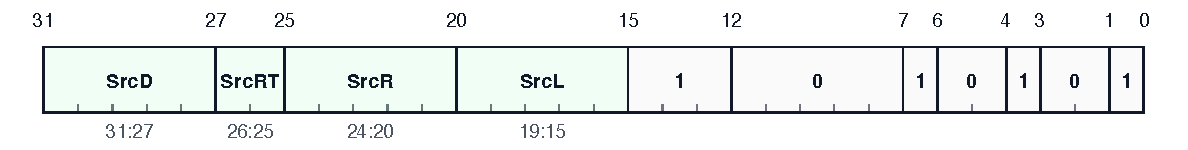
\includegraphics[width=\textwidth]{figs/encoding/scalar_instruction_entries/enc_sd_u.pdf}\par\smallskip
\begin{description}[leftmargin=0.18\linewidth,style=nextline]
\item[Format] \texttt{L32} \texttt{32-bit} scalar word.
\item[Pattern] \texttt{.................111000001001001}.
\end{description}
\noindent\textbf{Classification.}\par
\begin{description}[leftmargin=0.18\linewidth,style=nextline]
\item[Category] Load, Store, and Address Generation.
\item[Family] Store Register Offset.
\item[Execution class] \texttt{STA/BASE\_REG}; uop\_kind=AGU, agu\_kind=STA, addr\_mode=BASE\_REG, split=AGU+STD.
\end{description}
\noindent\textbf{Operand fields.}\par
\begin{description}[leftmargin=0.18\linewidth,style=nextline]
\item[\texttt{SrcD}] Bits \texttt{31:27 (5b)}. 5-bit scalar source register containing the data value written to memory; the instruction size selects the stored byte, halfword, word, or doubleword portion.
\item[\texttt{SrcL}] Bits \texttt{19:15 (5b)}. 5-bit scalar source register used as the base address for the memory access.
\item[\texttt{SrcR}] Bits \texttt{24:20 (5b)}. 5-bit scalar source register used as the register offset component of the effective address.
\item[\texttt{SrcRType}] Bits \texttt{26:25 (2b)}. 2-bit modifier for SrcR. It selects the encoded source form shown in the syntax, such as signed-word, unsigned-word, negated, or unmodified register input.
\end{description}
\noindent\textbf{Operation.}\par
\begin{lstlisting}[style=ptoscalarcode]
addr = ComputeAddress(/* per syntax */)
Store64(addr, Read(SrcD))
\end{lstlisting}
\Needspace{0.08\textheight}

\medskip
\input{scalar-instructions/entries/186_sdi.tex}
\medskip
% Scalar instruction entry source: tools/generate_scalar_instruction_catalog.py.
\subsection{\texttt{SDI.U}}
\label{sec:scalar-sdi_u}
\index{SDI.U@\texttt{SDI.U}}
\begin{sloppypar}\noindent\textbf{Purpose.} Stores a 64-bit value to memory using unscaled immediate-offset addressing.\end{sloppypar}\smallskip
\noindent\textbf{Syntax.}\par
\begin{lstlisting}[style=ptoscalarcode]
sdi.u SrcL, [SrcR, simm]
\end{lstlisting}
\noindent\textbf{Encoding.}\par
\noindent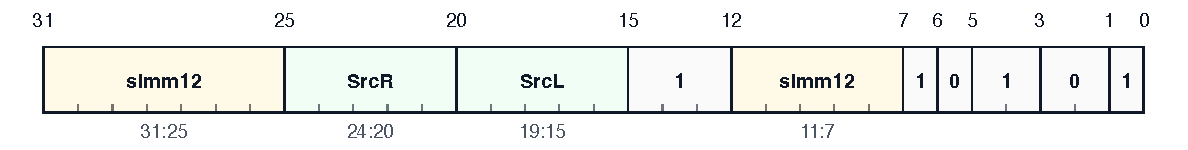
\includegraphics[width=\textwidth]{figs/encoding/scalar_instruction_entries/enc_sdi_u.pdf}\par\smallskip
\begin{description}[leftmargin=0.18\linewidth,style=nextline]
\item[Format] \texttt{L32} \texttt{32-bit} scalar word.
\item[Pattern] \texttt{.................111.....1011001}.
\end{description}
\noindent\textbf{Classification.}\par
\begin{description}[leftmargin=0.18\linewidth,style=nextline]
\item[Category] Load, Store, and Address Generation.
\item[Family] Store Immediate Offset.
\item[Execution class] \texttt{STA/BASE\_IMM}; uop\_kind=AGU, agu\_kind=STA, addr\_mode=BASE\_IMM, split=AGU+STD.
\end{description}
\noindent\textbf{Operand fields.}\par
\begin{description}[leftmargin=0.18\linewidth,style=nextline]
\item[\texttt{SrcL}] Bits \texttt{19:15 (5b)}. 5-bit scalar source register used as the base address for the memory access.
\item[\texttt{SrcR}] Bits \texttt{24:20 (5b)}. 5-bit scalar source register used as the register offset component of the effective address.
\item[\texttt{simm12}] Bits \texttt{31:25 (7b), 11:7 (5b)}. 12-bit signed address displacement added to the base register to form the effective address. The immediate is split across non-contiguous encoding slices and reassembled before use.
\end{description}
\noindent\textbf{Operation.}\par
\begin{lstlisting}[style=ptoscalarcode]
addr = ComputeAddress(/* per syntax */)
Store64(addr, Read(SrcL))
\end{lstlisting}
\Needspace{0.08\textheight}

\medskip
\input{scalar-instructions/entries/190_sh.tex}
\medskip
\input{scalar-instructions/entries/191_sh_pcr.tex}
\medskip
\input{scalar-instructions/entries/192_sh_u.tex}
\medskip
\input{scalar-instructions/entries/193_shi.tex}
\medskip
\input{scalar-instructions/entries/194_shi_u.tex}
\medskip
\input{scalar-instructions/entries/214_sw.tex}
\medskip
\input{scalar-instructions/entries/218_sw_pcr.tex}
\medskip
\input{scalar-instructions/entries/221_sw_u.tex}
\medskip
\input{scalar-instructions/entries/229_swi.tex}
\medskip
\input{scalar-instructions/entries/230_swi_u.tex}
\medskip

\section{Atomic Memory Operations}
Atomic memory operations perform load-reserved, store-conditional, swap, and arithmetic or logic read-modify-write transfers with encoded ordering qualifiers.\par\smallskip
{\scriptsize
\begin{longtable}{@{}L{0.24\linewidth}R{0.09\linewidth}L{0.56\linewidth}@{}}
\toprule
Family & Count & Representative instructions \\
\midrule
Atomic Operation & 44 & \texttt{LD.ADD, LD.AND, LD.OR, LD.SMAX, LD.SMIN, LD.UMAX, LD.UMIN, LD.XOR} \\
\bottomrule
\end{longtable}
}

\input{scalar-instructions/entries/105_ld_add.tex}
\medskip
\input{scalar-instructions/entries/106_ld_and.tex}
\medskip
\input{scalar-instructions/entries/107_ld_or.tex}
\medskip
\input{scalar-instructions/entries/109_ld_smax.tex}
\medskip
\input{scalar-instructions/entries/110_ld_smin.tex}
\medskip
\input{scalar-instructions/entries/111_ld_umax.tex}
\medskip
\input{scalar-instructions/entries/112_ld_umin.tex}
\medskip
\input{scalar-instructions/entries/113_ld_xor.tex}
\medskip
\input{scalar-instructions/entries/124_lr_b.tex}
\medskip
\input{scalar-instructions/entries/125_lr_d.tex}
\medskip
\input{scalar-instructions/entries/126_lr_h.tex}
\medskip
% Scalar instruction entry source: tools/generate_scalar_instruction_catalog.py.
\subsection{\texttt{LR.W}}
\label{sec:scalar-lr_w}
\index{LR.W@\texttt{LR.W}}
\begin{sloppypar}\noindent\textbf{Purpose.} Load-reserved: performs an atomic load and establishes a reservation for a subsequent store-conditional.\end{sloppypar}\smallskip
\noindent\textbf{Syntax.}\par
\begin{lstlisting}[style=ptoscalarcode]
lr.w<.{aq, rl, f, aqrl, aqf, rlf, aqrlf}> [SrcL], ->RegDst
\end{lstlisting}
\noindent\textbf{Encoding.}\par
\noindent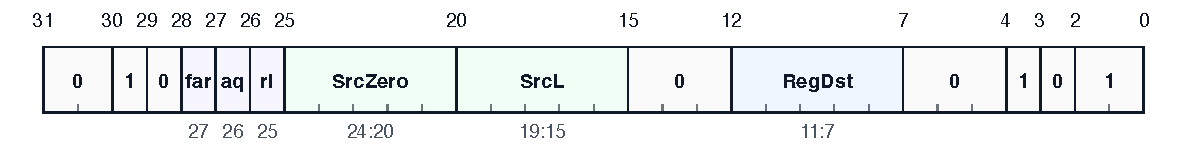
\includegraphics[width=\textwidth]{figs/encoding/scalar_instruction_entries/enc_lr_w.pdf}\par\smallskip
\begin{description}[leftmargin=0.18\linewidth,style=nextline]
\item[Format] \texttt{L32} \texttt{32-bit} scalar word.
\item[Pattern] \texttt{0010.............000.....0001011}.
\end{description}
\noindent\textbf{Classification.}\par
\begin{description}[leftmargin=0.18\linewidth,style=nextline]
\item[Category] Atomic Memory Operations.
\item[Family] Atomic Operation.
\item[Execution class] \texttt{AMO}; uop\_kind=AMO.
\end{description}
\noindent\textbf{Operand fields.}\par
\begin{description}[leftmargin=0.18\linewidth,style=nextline]
\item[\texttt{RegDst}] Bits \texttt{11:7 (5b)}. 5-bit scalar destination register that receives the original memory value returned by the atomic operation; X0 discards the returned value.
\item[\texttt{SrcL}] Bits \texttt{19:15 (5b)}. 5-bit scalar source register containing the memory address for the load-reserved operation.
\item[\texttt{SrcZero}] Bits \texttt{24:20 (5b)}. 5-bit source-register field that must encode X0; it occupies the standard source slot for encodings that do not consume a second register operand.
\item[\texttt{aq}] Bits \texttt{26:26 (1b)}. Acquire ordering bit for atomic memory operations. When set, later memory operations cannot be observed before this operation in the selected ordering domain.
\item[\texttt{far}] Bits \texttt{27:27 (1b)}. Atomic ordering-domain qualifier used with aq/rl suffixes; the assembly suffix containing f selects this encoded bit.
\item[\texttt{rl}] Bits \texttt{25:25 (1b)}. Release ordering bit for atomic memory operations. When set, earlier memory operations cannot be observed after this operation in the selected ordering domain.
\end{description}
\noindent\textbf{Operation.}\par
\begin{lstlisting}[style=ptoscalarcode]
addr = Read(SrcL)
value = LoadReserved32 (addr)
Write(RegDst, value)
\end{lstlisting}
\Needspace{0.08\textheight}

\medskip
\input{scalar-instructions/entries/131_lw_add.tex}
\medskip
\input{scalar-instructions/entries/132_lw_and.tex}
\medskip
\input{scalar-instructions/entries/133_lw_or.tex}
\medskip
\input{scalar-instructions/entries/135_lw_smax.tex}
\medskip
\input{scalar-instructions/entries/136_lw_smin.tex}
\medskip
\input{scalar-instructions/entries/137_lw_umax.tex}
\medskip
% Scalar instruction entry source: tools/generate_scalar_instruction_catalog.py.
\subsection{\texttt{LW.UMIN}}
\label{sec:scalar-lw_umin}
\index{LW.UMIN@\texttt{LW.UMIN}}
\begin{sloppypar}\noindent\textbf{Purpose.} Atomic read-modify-write operation that returns the original memory value.\end{sloppypar}\smallskip
\noindent\textbf{Syntax.}\par
\begin{lstlisting}[style=ptoscalarcode]
lw.umin<.{aq, rl, f, aqrl, aqf, rlf, aqrlf}> [SrcL], SrcR, ->RegDst
\end{lstlisting}
\noindent\textbf{Encoding.}\par
\noindent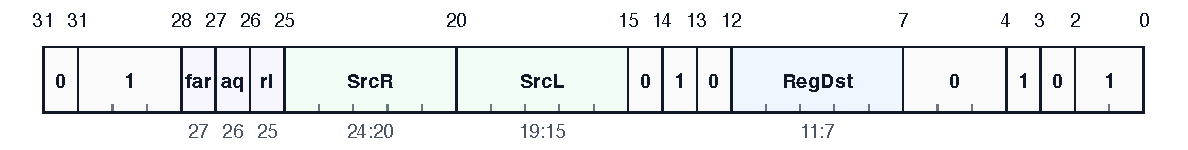
\includegraphics[width=\textwidth]{figs/encoding/scalar_instruction_entries/enc_lw_umin.pdf}\par\smallskip
\begin{description}[leftmargin=0.18\linewidth,style=nextline]
\item[Format] \texttt{L32} \texttt{32-bit} scalar word.
\item[Pattern] \texttt{0111.............010.....0001011}.
\end{description}
\noindent\textbf{Classification.}\par
\begin{description}[leftmargin=0.18\linewidth,style=nextline]
\item[Category] Atomic Memory Operations.
\item[Family] Atomic Operation.
\item[Execution class] \texttt{AMO}; uop\_kind=AMO.
\end{description}
\noindent\textbf{Operand fields.}\par
\begin{description}[leftmargin=0.18\linewidth,style=nextline]
\item[\texttt{RegDst}] Bits \texttt{11:7 (5b)}. 5-bit scalar destination register that receives the original memory value returned by the atomic operation; X0 discards the returned value.
\item[\texttt{SrcL}] Bits \texttt{19:15 (5b)}. 5-bit scalar source register containing the memory address for the atomic read-modify-write operation.
\item[\texttt{SrcR}] Bits \texttt{24:20 (5b)}. 5-bit scalar source register containing the update operand for the atomic read-modify-write operation.
\item[\texttt{aq}] Bits \texttt{26:26 (1b)}. Acquire ordering bit for atomic memory operations. When set, later memory operations cannot be observed before this operation in the selected ordering domain.
\item[\texttt{far}] Bits \texttt{27:27 (1b)}. Atomic ordering-domain qualifier used with aq/rl suffixes; the assembly suffix containing f selects this encoded bit.
\item[\texttt{rl}] Bits \texttt{25:25 (1b)}. Release ordering bit for atomic memory operations. When set, earlier memory operations cannot be observed after this operation in the selected ordering domain.
\end{description}
\noindent\textbf{Operation.}\par
\begin{lstlisting}[style=ptoscalarcode]
addr = Read(SrcL)
old = AtomicLoad32(addr)
new = umin(old, Read(SrcR))
AtomicStore32(addr, new)
Write(RegDst, old)
\end{lstlisting}
\Needspace{0.08\textheight}

\medskip
\input{scalar-instructions/entries/139_lw_xor.tex}
\medskip
\input{scalar-instructions/entries/170_sc_b.tex}
\medskip
% Scalar instruction entry source: tools/generate_scalar_instruction_catalog.py.
\subsection{\texttt{SC.D}}
\label{sec:scalar-sc_d}
\index{SC.D@\texttt{SC.D}}
\begin{sloppypar}\noindent\textbf{Purpose.} Store-conditional: attempts an atomic store that succeeds only if the reservation is still valid; returns a status code.\end{sloppypar}\smallskip
\noindent\textbf{Syntax.}\par
\begin{lstlisting}[style=ptoscalarcode]
sc.d<.{aq, rl, f, aqrl, aqf, rlf, aqrlf}> SrcL, [SrcR], ->RegDst
\end{lstlisting}
\noindent\textbf{Encoding.}\par
\noindent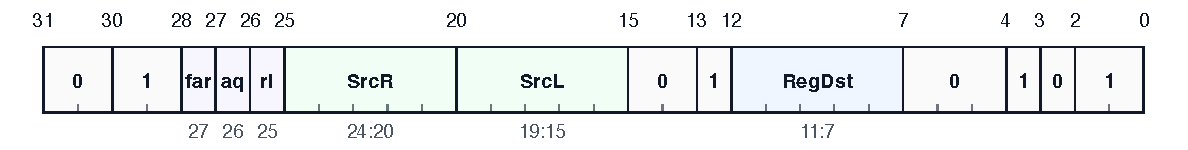
\includegraphics[width=\textwidth]{figs/encoding/scalar_instruction_entries/enc_sc_d.pdf}\par\smallskip
\begin{description}[leftmargin=0.18\linewidth,style=nextline]
\item[Format] \texttt{L32} \texttt{32-bit} scalar word.
\item[Pattern] \texttt{0011.............001.....0001011}.
\end{description}
\noindent\textbf{Classification.}\par
\begin{description}[leftmargin=0.18\linewidth,style=nextline]
\item[Category] Atomic Memory Operations.
\item[Family] Atomic Operation.
\item[Execution class] \texttt{AMO}; uop\_kind=AMO.
\end{description}
\noindent\textbf{Operand fields.}\par
\begin{description}[leftmargin=0.18\linewidth,style=nextline]
\item[\texttt{RegDst}] Bits \texttt{11:7 (5b)}. 5-bit scalar destination register that receives the store-conditional status code; X0 discards the status write.
\item[\texttt{SrcL}] Bits \texttt{19:15 (5b)}. 5-bit scalar source register containing the value to store if the reservation check succeeds.
\item[\texttt{SrcR}] Bits \texttt{24:20 (5b)}. 5-bit scalar source register containing the memory address checked against the active reservation.
\item[\texttt{aq}] Bits \texttt{26:26 (1b)}. Acquire ordering bit for atomic memory operations. When set, later memory operations cannot be observed before this operation in the selected ordering domain.
\item[\texttt{far}] Bits \texttt{27:27 (1b)}. Atomic ordering-domain qualifier used with aq/rl suffixes; the assembly suffix containing f selects this encoded bit.
\item[\texttt{rl}] Bits \texttt{25:25 (1b)}. Release ordering bit for atomic memory operations. When set, earlier memory operations cannot be observed after this operation in the selected ordering domain.
\end{description}
\noindent\textbf{Operation.}\par
\begin{lstlisting}[style=ptoscalarcode]
addr = Read(SrcR)
status = StoreConditional64(addr, Read(SrcL))
Write(RegDst, status)
\end{lstlisting}
\Needspace{0.08\textheight}

\medskip
\input{scalar-instructions/entries/172_sc_h.tex}
\medskip
\input{scalar-instructions/entries/173_sc_w.tex}
\medskip
\input{scalar-instructions/entries/176_sd_add.tex}
\medskip
\input{scalar-instructions/entries/177_sd_and.tex}
\medskip
% Scalar instruction entry source: tools/generate_scalar_instruction_catalog.py.
\subsection{\texttt{SD.OR}}
\label{sec:scalar-sd_or}
\index{SD.OR@\texttt{SD.OR}}
\begin{sloppypar}\noindent\textbf{Purpose.} Atomic read-modify-write operation that updates memory without returning a value.\end{sloppypar}\smallskip
\noindent\textbf{Syntax.}\par
\begin{lstlisting}[style=ptoscalarcode]
sd.or<.{rl, f, rlf}> [SrcL], SrcR
\end{lstlisting}
\noindent\textbf{Encoding.}\par
\noindent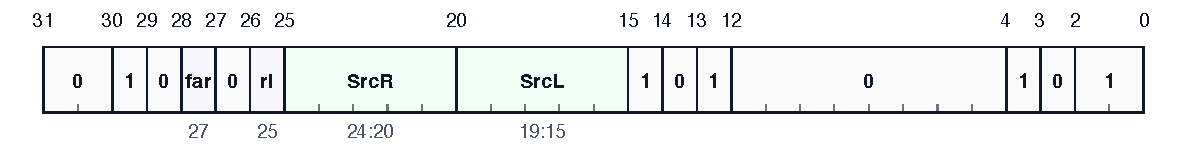
\includegraphics[width=\textwidth]{figs/encoding/scalar_instruction_entries/enc_sd_or.pdf}\par\smallskip
\begin{description}[leftmargin=0.18\linewidth,style=nextline]
\item[Format] \texttt{L32} \texttt{32-bit} scalar word.
\item[Pattern] \texttt{0010.0...........101000000001011}.
\end{description}
\noindent\textbf{Classification.}\par
\begin{description}[leftmargin=0.18\linewidth,style=nextline]
\item[Category] Atomic Memory Operations.
\item[Family] Atomic Operation.
\item[Execution class] \texttt{AMO}; uop\_kind=AMO.
\end{description}
\noindent\textbf{Operand fields.}\par
\begin{description}[leftmargin=0.18\linewidth,style=nextline]
\item[\texttt{SrcL}] Bits \texttt{19:15 (5b)}. 5-bit scalar source register containing the memory address for the atomic read-modify-write operation.
\item[\texttt{SrcR}] Bits \texttt{24:20 (5b)}. 5-bit scalar source register containing the update operand for the atomic read-modify-write operation.
\item[\texttt{far}] Bits \texttt{27:27 (1b)}. Atomic ordering-domain qualifier used with aq/rl suffixes; the assembly suffix containing f selects this encoded bit.
\item[\texttt{rl}] Bits \texttt{25:25 (1b)}. Release ordering bit for atomic memory operations. When set, earlier memory operations cannot be observed after this operation in the selected ordering domain.
\end{description}
\noindent\textbf{Operation.}\par
\begin{lstlisting}[style=ptoscalarcode]
addr = Read(SrcL)
old = AtomicLoad64(addr)
new = old | Read(SrcR)
AtomicStore64(addr, new)
\end{lstlisting}
\Needspace{0.08\textheight}

\medskip
\input{scalar-instructions/entries/180_sd_smax.tex}
\medskip
\input{scalar-instructions/entries/181_sd_smin.tex}
\medskip
\input{scalar-instructions/entries/183_sd_umax.tex}
\medskip
\input{scalar-instructions/entries/184_sd_umin.tex}
\medskip
\input{scalar-instructions/entries/185_sd_xor.tex}
\medskip
\input{scalar-instructions/entries/215_sw_add.tex}
\medskip
\input{scalar-instructions/entries/216_sw_and.tex}
\medskip
% Scalar instruction entry source: tools/generate_scalar_instruction_catalog.py.
\subsection{\texttt{SW.OR}}
\label{sec:scalar-sw_or}
\index{SW.OR@\texttt{SW.OR}}
\begin{sloppypar}\noindent\textbf{Purpose.} Atomic read-modify-write operation that updates memory without returning a value.\end{sloppypar}\smallskip
\noindent\textbf{Syntax.}\par
\begin{lstlisting}[style=ptoscalarcode]
sw.or<.{rl, f, rlf}> [SrcL], SrcR
\end{lstlisting}
\noindent\textbf{Encoding.}\par
\noindent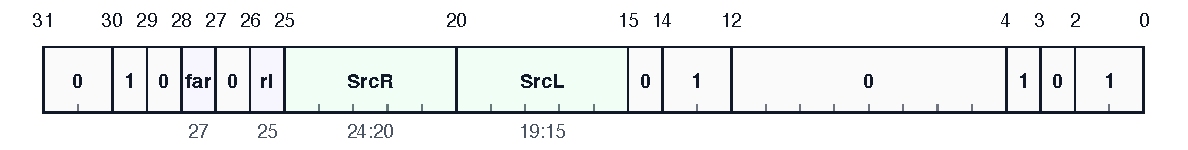
\includegraphics[width=\textwidth]{figs/encoding/scalar_instruction_entries/enc_sw_or.pdf}\par\smallskip
\begin{description}[leftmargin=0.18\linewidth,style=nextline]
\item[Format] \texttt{L32} \texttt{32-bit} scalar word.
\item[Pattern] \texttt{0010.0...........011000000001011}.
\end{description}
\noindent\textbf{Classification.}\par
\begin{description}[leftmargin=0.18\linewidth,style=nextline]
\item[Category] Atomic Memory Operations.
\item[Family] Atomic Operation.
\item[Execution class] \texttt{AMO}; uop\_kind=AMO.
\end{description}
\noindent\textbf{Operand fields.}\par
\begin{description}[leftmargin=0.18\linewidth,style=nextline]
\item[\texttt{SrcL}] Bits \texttt{19:15 (5b)}. 5-bit scalar source register containing the memory address for the atomic read-modify-write operation.
\item[\texttt{SrcR}] Bits \texttt{24:20 (5b)}. 5-bit scalar source register containing the update operand for the atomic read-modify-write operation.
\item[\texttt{far}] Bits \texttt{27:27 (1b)}. Atomic ordering-domain qualifier used with aq/rl suffixes; the assembly suffix containing f selects this encoded bit.
\item[\texttt{rl}] Bits \texttt{25:25 (1b)}. Release ordering bit for atomic memory operations. When set, earlier memory operations cannot be observed after this operation in the selected ordering domain.
\end{description}
\noindent\textbf{Operation.}\par
\begin{lstlisting}[style=ptoscalarcode]
addr = Read(SrcL)
old = AtomicLoad32(addr)
new = old | Read(SrcR)
AtomicStore32(addr, new)
\end{lstlisting}
\Needspace{0.08\textheight}

\medskip
\input{scalar-instructions/entries/219_sw_smax.tex}
\medskip
\input{scalar-instructions/entries/220_sw_smin.tex}
\medskip
\input{scalar-instructions/entries/222_sw_umax.tex}
\medskip
\input{scalar-instructions/entries/223_sw_umin.tex}
\medskip
\input{scalar-instructions/entries/224_sw_xor.tex}
\medskip
\input{scalar-instructions/entries/225_swapb.tex}
\medskip
\input{scalar-instructions/entries/226_swapd.tex}
\medskip
\input{scalar-instructions/entries/227_swaph.tex}
\medskip
\input{scalar-instructions/entries/228_swapw.tex}
\medskip

\section{Floating-Point and Conversion}
Floating-point and conversion instructions execute scalar FP arithmetic, FP compares, and integer/FP format conversions.\par\smallskip
{\scriptsize
\begin{longtable}{@{}L{0.24\linewidth}R{0.09\linewidth}L{0.56\linewidth}@{}}
\toprule
Family & Count & Representative instructions \\
\midrule
Floating-point Arithmetic & 12 & \texttt{FABS, FADD, FDIV, FEXP, FMADD, FMSUB, FMUL, FNMADD} \\
Floating-point Compare & 8 & \texttt{FEQ, FEQS, FGE, FGES, FLT, FLTS, FNE, FNES} \\
Format Convert & 8 & \texttt{FCVT, FCVTA, FCVTM, FCVTN, FCVTP, FCVTZ, SCVTF, UCVTF} \\
Max-Min & 2 & \texttt{FMAX, FMIN} \\
\bottomrule
\end{longtable}
}

% Scalar instruction entry source: tools/generate_scalar_instruction_catalog.py.
\subsection{\texttt{FABS}}
\label{sec:scalar-fabs}
\index{FABS@\texttt{FABS}}
\begin{sloppypar}\noindent\textbf{Purpose.} Clears the sign bit of the floating-point source operand and writes the absolute value to RegDst.\end{sloppypar}\smallskip
\noindent\textbf{Syntax.}\par
\begin{lstlisting}[style=ptoscalarcode]
fabs.{T} SrcL, ->RegDst
\end{lstlisting}
\noindent\textbf{Encoding.}\par
\noindent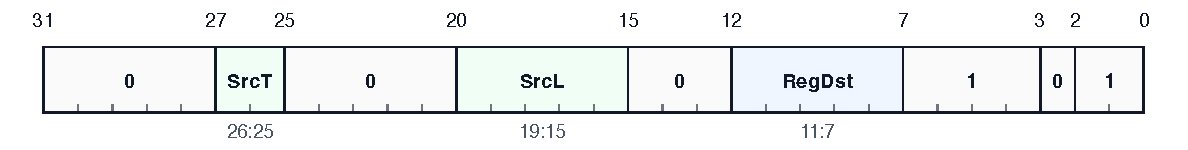
\includegraphics[width=\textwidth]{figs/encoding/scalar_instruction_entries/enc_fabs.pdf}\par\smallskip
\begin{description}[leftmargin=0.18\linewidth,style=nextline]
\item[Format] \texttt{L32} \texttt{32-bit} scalar word.
\item[Pattern] \texttt{00000..00000.....000.....1111011}.
\end{description}
\noindent\textbf{Classification.}\par
\begin{description}[leftmargin=0.18\linewidth,style=nextline]
\item[Category] Floating-Point and Conversion.
\item[Family] Floating-point Arithmetic.
\item[Execution class] \texttt{FSU}; uop\_kind=FSU.
\end{description}
\noindent\textbf{Operand fields.}\par
\begin{description}[leftmargin=0.18\linewidth,style=nextline]
\item[\texttt{RegDst}] Bits \texttt{11:7 (5b)}. 5-bit scalar destination register that receives the floating-point, conversion, or FP-compare result encoded in scalar register storage; X0 discards the write.
\item[\texttt{SrcL}] Bits \texttt{19:15 (5b)}. 5-bit scalar source register holding the left or only floating-point/conversion operand; SrcType or the assembly suffix determines the interpreted format.
\item[\texttt{SrcType}] Bits \texttt{26:25 (2b)}. 2-bit source format selector for floating-point or conversion operands. The assembly suffix \{T\} names the selected floating-point element format.
\end{description}
\noindent\textbf{Operation.}\par
\begin{lstlisting}[style=ptoscalarcode]
a = Read(SrcL)
// clear sign bit (fd: bit63; fs: bit31 in low word)
result = Abs(a)
Write(RegDst, result)
\end{lstlisting}
\Needspace{0.08\textheight}

\medskip
\input{scalar-instructions/entries/065_fadd.tex}
\medskip
% Scalar instruction entry source: tools/generate_scalar_instruction_catalog.py.
\subsection{\texttt{FCVT}}
\label{sec:scalar-fcvt}
\index{FCVT@\texttt{FCVT}}
\begin{sloppypar}\noindent\textbf{Purpose.} Converts SrcL between encoded floating-point formats using the default rounding mode and writes the result to RegDst.\end{sloppypar}\smallskip
\noindent\textbf{Syntax.}\par
\begin{lstlisting}[style=ptoscalarcode]
fcvt.{srcT2dstT} SrcL, ->RegDst
\end{lstlisting}
\noindent\textbf{Encoding.}\par
\noindent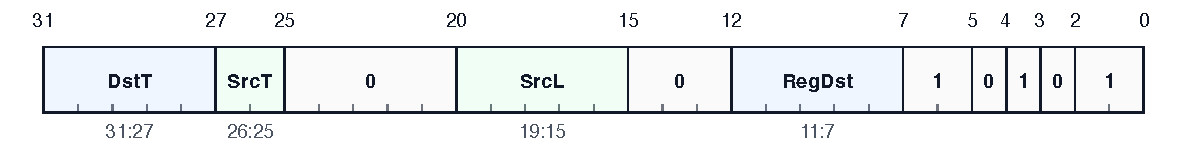
\includegraphics[width=\textwidth]{figs/encoding/scalar_instruction_entries/enc_fcvt.pdf}\par\smallskip
\begin{description}[leftmargin=0.18\linewidth,style=nextline]
\item[Format] \texttt{L32} \texttt{32-bit} scalar word.
\item[Pattern] \texttt{.......00000.....000.....1101011}.
\end{description}
\noindent\textbf{Classification.}\par
\begin{description}[leftmargin=0.18\linewidth,style=nextline]
\item[Category] Floating-Point and Conversion.
\item[Family] Format Convert.
\item[Execution class] \texttt{FSU}; uop\_kind=FSU.
\end{description}
\noindent\textbf{Operand fields.}\par
\begin{description}[leftmargin=0.18\linewidth,style=nextline]
\item[\texttt{DstType}] Bits \texttt{31:27 (5b)}. 5-bit destination format selector for conversion results. The assembly suffix \{srcT2dstT\} names the source and destination formats.
\item[\texttt{RegDst}] Bits \texttt{11:7 (5b)}. 5-bit scalar destination register that receives the floating-point, conversion, or FP-compare result encoded in scalar register storage; X0 discards the write.
\item[\texttt{SrcL}] Bits \texttt{19:15 (5b)}. 5-bit scalar source register holding the left or only floating-point/conversion operand; SrcType or the assembly suffix determines the interpreted format.
\item[\texttt{SrcType}] Bits \texttt{26:25 (2b)}. 2-bit source format selector for floating-point or conversion operands. The assembly suffix \{srcT2dstT\} names the source and destination formats.
\end{description}
\noindent\textbf{Operation.}\par
\begin{lstlisting}[style=ptoscalarcode]
value = Read(SrcL)
Write(RegDst, ConvertFormat(value, srcT, dstT, default_rounding))
\end{lstlisting}
\Needspace{0.08\textheight}

\medskip
\input{scalar-instructions/entries/067_fcvta.tex}
\medskip
\input{scalar-instructions/entries/068_fcvtm.tex}
\medskip
% Scalar instruction entry source: tools/generate_scalar_instruction_catalog.py.
\subsection{\texttt{FCVTN}}
\label{sec:scalar-fcvtn}
\index{FCVTN@\texttt{FCVTN}}
\begin{sloppypar}\noindent\textbf{Purpose.} Converts SrcL between encoded numeric formats using round-to-nearest and writes the result to RegDst.\end{sloppypar}\smallskip
\noindent\textbf{Syntax.}\par
\begin{lstlisting}[style=ptoscalarcode]
fcvtn.{srcT2dstT} SrcL, ->RegDst
\end{lstlisting}
\noindent\textbf{Encoding.}\par
\noindent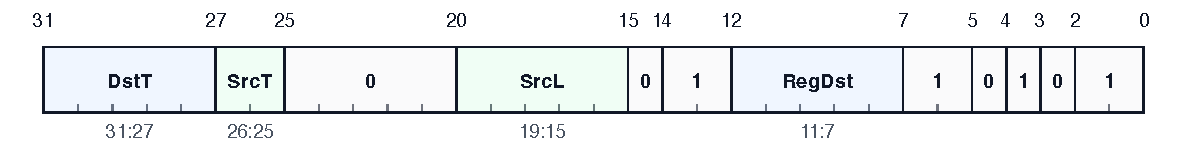
\includegraphics[width=\textwidth]{figs/encoding/scalar_instruction_entries/enc_fcvtn.pdf}\par\smallskip
\begin{description}[leftmargin=0.18\linewidth,style=nextline]
\item[Format] \texttt{L32} \texttt{32-bit} scalar word.
\item[Pattern] \texttt{.......00000.....011.....1101011}.
\end{description}
\noindent\textbf{Classification.}\par
\begin{description}[leftmargin=0.18\linewidth,style=nextline]
\item[Category] Floating-Point and Conversion.
\item[Family] Format Convert.
\item[Execution class] \texttt{FSU}; uop\_kind=FSU.
\end{description}
\noindent\textbf{Operand fields.}\par
\begin{description}[leftmargin=0.18\linewidth,style=nextline]
\item[\texttt{DstType}] Bits \texttt{31:27 (5b)}. 5-bit destination format selector for conversion results. The assembly suffix \{srcT2dstT\} names the source and destination formats.
\item[\texttt{RegDst}] Bits \texttt{11:7 (5b)}. 5-bit scalar destination register that receives the floating-point, conversion, or FP-compare result encoded in scalar register storage; X0 discards the write.
\item[\texttt{SrcL}] Bits \texttt{19:15 (5b)}. 5-bit scalar source register holding the left or only floating-point/conversion operand; SrcType or the assembly suffix determines the interpreted format.
\item[\texttt{SrcType}] Bits \texttt{26:25 (2b)}. 2-bit source format selector for floating-point or conversion operands. The assembly suffix \{srcT2dstT\} names the source and destination formats.
\end{description}
\noindent\textbf{Operation.}\par
\begin{lstlisting}[style=ptoscalarcode]
value = Read(SrcL)
Write(RegDst, ConvertFormat(value, srcT, dstT, round_to_nearest))
\end{lstlisting}
\Needspace{0.08\textheight}

\medskip
\input{scalar-instructions/entries/070_fcvtp.tex}
\medskip
\input{scalar-instructions/entries/071_fcvtz.tex}
\medskip
% Scalar instruction entry source: tools/generate_scalar_instruction_catalog.py.
\subsection{\texttt{FDIV}}
\label{sec:scalar-fdiv}
\index{FDIV@\texttt{FDIV}}
\begin{sloppypar}\noindent\textbf{Purpose.} Divides the floating-point left operand by the right operand and writes the rounded result to RegDst.\end{sloppypar}\smallskip
\noindent\textbf{Syntax.}\par
\begin{lstlisting}[style=ptoscalarcode]
fdiv.{T} SrcL, SrcR, ->RegDst
\end{lstlisting}
\noindent\textbf{Encoding.}\par
\noindent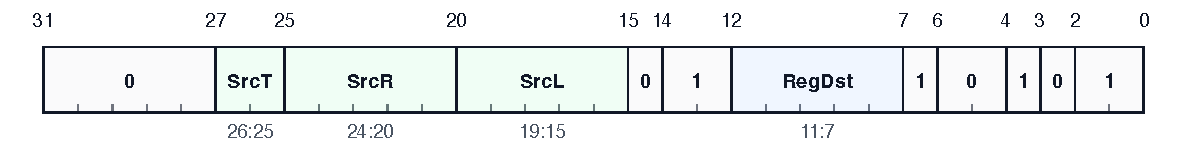
\includegraphics[width=\textwidth]{figs/encoding/scalar_instruction_entries/enc_fdiv.pdf}\par\smallskip
\begin{description}[leftmargin=0.18\linewidth,style=nextline]
\item[Format] \texttt{L32} \texttt{32-bit} scalar word.
\item[Pattern] \texttt{00000............011.....1001011}.
\end{description}
\noindent\textbf{Classification.}\par
\begin{description}[leftmargin=0.18\linewidth,style=nextline]
\item[Category] Floating-Point and Conversion.
\item[Family] Floating-point Arithmetic.
\item[Execution class] \texttt{FSU}; uop\_kind=FSU.
\end{description}
\noindent\textbf{Operand fields.}\par
\begin{description}[leftmargin=0.18\linewidth,style=nextline]
\item[\texttt{RegDst}] Bits \texttt{11:7 (5b)}. 5-bit scalar destination register that receives the floating-point, conversion, or FP-compare result encoded in scalar register storage; X0 discards the write.
\item[\texttt{SrcL}] Bits \texttt{19:15 (5b)}. 5-bit scalar source register holding the left or only floating-point/conversion operand; SrcType or the assembly suffix determines the interpreted format.
\item[\texttt{SrcR}] Bits \texttt{24:20 (5b)}. 5-bit scalar source register holding the right floating-point operand.
\item[\texttt{SrcType}] Bits \texttt{26:25 (2b)}. 2-bit source format selector for floating-point or conversion operands. The assembly suffix \{T\} names the selected floating-point element format.
\end{description}
\noindent\textbf{Operation.}\par
\begin{lstlisting}[style=ptoscalarcode]
lhs = FPRead(SrcL, T)
rhs = FPRead(SrcR, T)
Write(RegDst, FPRound(lhs / rhs, T))
\end{lstlisting}
\Needspace{0.08\textheight}

\medskip
\input{scalar-instructions/entries/075_feq.tex}
\medskip
\input{scalar-instructions/entries/076_feqs.tex}
\medskip
% Scalar instruction entry source: tools/generate_scalar_instruction_catalog.py.
\subsection{\texttt{FEXP}}
\label{sec:scalar-fexp}
\index{FEXP@\texttt{FEXP}}
\begin{sloppypar}\noindent\textbf{Purpose.} Computes the floating-point exponential of SrcL and writes the rounded result to RegDst.\end{sloppypar}\smallskip
\noindent\textbf{Syntax.}\par
\begin{lstlisting}[style=ptoscalarcode]
fexp.{T} SrcL, ->RegDst
\end{lstlisting}
\noindent\textbf{Encoding.}\par
\noindent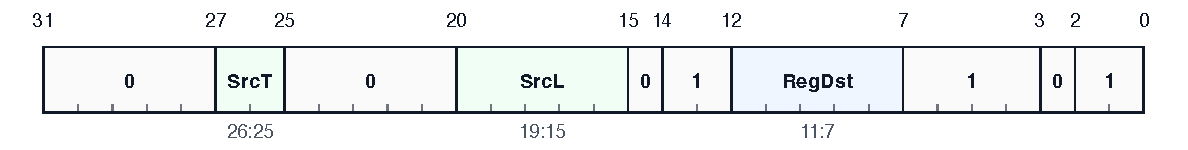
\includegraphics[width=\textwidth]{figs/encoding/scalar_instruction_entries/enc_fexp.pdf}\par\smallskip
\begin{description}[leftmargin=0.18\linewidth,style=nextline]
\item[Format] \texttt{L32} \texttt{32-bit} scalar word.
\item[Pattern] \texttt{00000..00000.....011.....1111011}.
\end{description}
\noindent\textbf{Classification.}\par
\begin{description}[leftmargin=0.18\linewidth,style=nextline]
\item[Category] Floating-Point and Conversion.
\item[Family] Floating-point Arithmetic.
\item[Execution class] \texttt{FSU}; uop\_kind=FSU.
\end{description}
\noindent\textbf{Operand fields.}\par
\begin{description}[leftmargin=0.18\linewidth,style=nextline]
\item[\texttt{RegDst}] Bits \texttt{11:7 (5b)}. 5-bit scalar destination register that receives the floating-point, conversion, or FP-compare result encoded in scalar register storage; X0 discards the write.
\item[\texttt{SrcL}] Bits \texttt{19:15 (5b)}. 5-bit scalar source register holding the left or only floating-point/conversion operand; SrcType or the assembly suffix determines the interpreted format.
\item[\texttt{SrcType}] Bits \texttt{26:25 (2b)}. 2-bit source format selector for floating-point or conversion operands. The assembly suffix \{T\} names the selected floating-point element format.
\end{description}
\noindent\textbf{Operation.}\par
\begin{lstlisting}[style=ptoscalarcode]
value = FPRead(SrcL, T)
Write(RegDst, FPRound(exp(value), T))
\end{lstlisting}
\Needspace{0.08\textheight}

\medskip
\input{scalar-instructions/entries/078_fge.tex}
\medskip
% Scalar instruction entry source: tools/generate_scalar_instruction_catalog.py.
\subsection{\texttt{FGES}}
\label{sec:scalar-fges}
\index{FGES@\texttt{FGES}}
\begin{sloppypar}\noindent\textbf{Purpose.} Performs a signaling floating-point greater-than-or-equal comparison and writes 1 or 0 to RegDst.\end{sloppypar}\smallskip
\noindent\textbf{Syntax.}\par
\begin{lstlisting}[style=ptoscalarcode]
fges.{T} SrcL, SrcR, ->RegDst
\end{lstlisting}
\noindent\textbf{Encoding.}\par
\noindent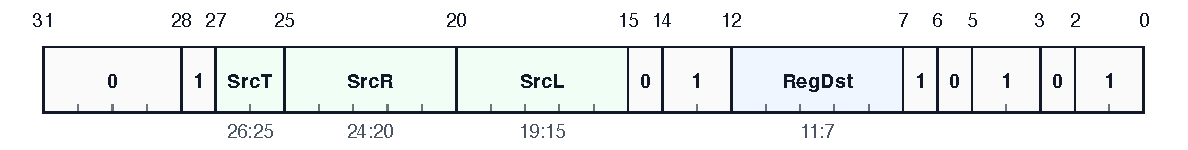
\includegraphics[width=\textwidth]{figs/encoding/scalar_instruction_entries/enc_fges.pdf}\par\smallskip
\begin{description}[leftmargin=0.18\linewidth,style=nextline]
\item[Format] \texttt{L32} \texttt{32-bit} scalar word.
\item[Pattern] \texttt{00001............011.....1011011}.
\end{description}
\noindent\textbf{Classification.}\par
\begin{description}[leftmargin=0.18\linewidth,style=nextline]
\item[Category] Floating-Point and Conversion.
\item[Family] Floating-point Compare.
\item[Execution class] \texttt{FSU}; uop\_kind=FSU.
\end{description}
\noindent\textbf{Operand fields.}\par
\begin{description}[leftmargin=0.18\linewidth,style=nextline]
\item[\texttt{RegDst}] Bits \texttt{11:7 (5b)}. 5-bit scalar destination register that receives the boolean compare result, encoded as 1 for true and 0 for false; X0 discards the write.
\item[\texttt{SrcL}] Bits \texttt{19:15 (5b)}. 5-bit scalar source register holding the left or only floating-point/conversion operand; SrcType or the assembly suffix determines the interpreted format.
\item[\texttt{SrcR}] Bits \texttt{24:20 (5b)}. 5-bit scalar source register holding the right floating-point operand.
\item[\texttt{SrcType}] Bits \texttt{26:25 (2b)}. 2-bit source format selector for floating-point or conversion operands. The assembly suffix \{T\} names the selected floating-point element format.
\end{description}
\noindent\textbf{Operation.}\par
\begin{lstlisting}[style=ptoscalarcode]
a = Read(SrcL)  // fd: full 64b; fs: low 32b
b = Read(SrcR)
// SrcType selects fd/fs; NaNs make predicate false
result = OrderedGe(a, b) ? 1 : 0
Write(RegDst, result)
\end{lstlisting}
\Needspace{0.08\textheight}

\medskip
\input{scalar-instructions/entries/080_flt.tex}
\medskip
\input{scalar-instructions/entries/081_flts.tex}
\medskip
\input{scalar-instructions/entries/082_fmadd.tex}
\medskip
\input{scalar-instructions/entries/083_fmax.tex}
\medskip
\input{scalar-instructions/entries/084_fmin.tex}
\medskip
\input{scalar-instructions/entries/085_fmsub.tex}
\medskip
\input{scalar-instructions/entries/086_fmul.tex}
\medskip
\input{scalar-instructions/entries/087_fne.tex}
\medskip
\input{scalar-instructions/entries/088_fnes.tex}
\medskip
\input{scalar-instructions/entries/089_fnmadd.tex}
\medskip
\input{scalar-instructions/entries/090_fnmsub.tex}
\medskip
\input{scalar-instructions/entries/091_frecip.tex}
\medskip
% Scalar instruction entry source: tools/generate_scalar_instruction_catalog.py.
\subsection{\texttt{FSQRT}}
\label{sec:scalar-fsqrt}
\index{FSQRT@\texttt{FSQRT}}
\begin{sloppypar}\noindent\textbf{Purpose.} Computes the square root of the floating-point source operand and writes the rounded result to RegDst.\end{sloppypar}\smallskip
\noindent\textbf{Syntax.}\par
\begin{lstlisting}[style=ptoscalarcode]
fsqrt.{T} SrcL, ->RegDst
\end{lstlisting}
\noindent\textbf{Encoding.}\par
\noindent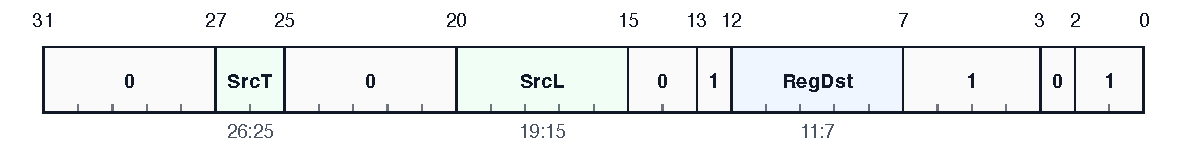
\includegraphics[width=\textwidth]{figs/encoding/scalar_instruction_entries/enc_fsqrt.pdf}\par\smallskip
\begin{description}[leftmargin=0.18\linewidth,style=nextline]
\item[Format] \texttt{L32} \texttt{32-bit} scalar word.
\item[Pattern] \texttt{00000..00000.....001.....1111011}.
\end{description}
\noindent\textbf{Classification.}\par
\begin{description}[leftmargin=0.18\linewidth,style=nextline]
\item[Category] Floating-Point and Conversion.
\item[Family] Floating-point Arithmetic.
\item[Execution class] \texttt{FSU}; uop\_kind=FSU.
\end{description}
\noindent\textbf{Operand fields.}\par
\begin{description}[leftmargin=0.18\linewidth,style=nextline]
\item[\texttt{RegDst}] Bits \texttt{11:7 (5b)}. 5-bit scalar destination register that receives the floating-point, conversion, or FP-compare result encoded in scalar register storage; X0 discards the write.
\item[\texttt{SrcL}] Bits \texttt{19:15 (5b)}. 5-bit scalar source register holding the left or only floating-point/conversion operand; SrcType or the assembly suffix determines the interpreted format.
\item[\texttt{SrcType}] Bits \texttt{26:25 (2b)}. 2-bit source format selector for floating-point or conversion operands. The assembly suffix \{T\} names the selected floating-point element format.
\end{description}
\noindent\textbf{Operation.}\par
\begin{lstlisting}[style=ptoscalarcode]
value = FPRead(SrcL, T)
Write(RegDst, FPRound(sqrt(value), T))
\end{lstlisting}
\Needspace{0.08\textheight}

\medskip
\input{scalar-instructions/entries/093_fsub.tex}
\medskip
\input{scalar-instructions/entries/174_scvtf.tex}
\medskip
% Scalar instruction entry source: tools/generate_scalar_instruction_catalog.py.
\subsection{\texttt{UCVTF}}
\label{sec:scalar-ucvtf}
\index{UCVTF@\texttt{UCVTF}}
\begin{sloppypar}\noindent\textbf{Purpose.} Converts an unsigned integer source value to the selected floating-point destination format.\end{sloppypar}\smallskip
\noindent\textbf{Syntax.}\par
\begin{lstlisting}[style=ptoscalarcode]
ucvtf.{srcT2dstT} SrcL, ->RegDst
\end{lstlisting}
\noindent\textbf{Encoding.}\par
\noindent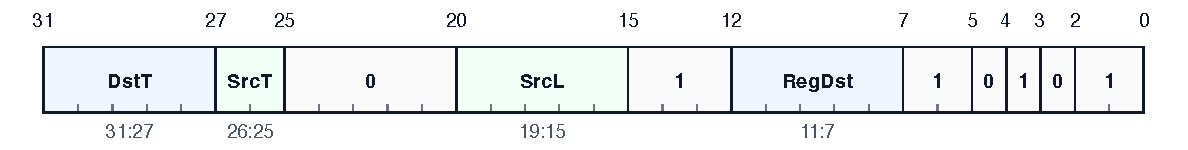
\includegraphics[width=\textwidth]{figs/encoding/scalar_instruction_entries/enc_ucvtf.pdf}\par\smallskip
\begin{description}[leftmargin=0.18\linewidth,style=nextline]
\item[Format] \texttt{L32} \texttt{32-bit} scalar word.
\item[Pattern] \texttt{.......00000.....111.....1101011}.
\end{description}
\noindent\textbf{Classification.}\par
\begin{description}[leftmargin=0.18\linewidth,style=nextline]
\item[Category] Floating-Point and Conversion.
\item[Family] Format Convert.
\item[Execution class] \texttt{FSU}; uop\_kind=FSU.
\end{description}
\noindent\textbf{Operand fields.}\par
\begin{description}[leftmargin=0.18\linewidth,style=nextline]
\item[\texttt{DstType}] Bits \texttt{31:27 (5b)}. 5-bit destination format selector for conversion results. The assembly suffix \{srcT2dstT\} names the source and destination formats.
\item[\texttt{RegDst}] Bits \texttt{11:7 (5b)}. 5-bit scalar destination register that receives the floating-point, conversion, or FP-compare result encoded in scalar register storage; X0 discards the write.
\item[\texttt{SrcL}] Bits \texttt{19:15 (5b)}. 5-bit scalar source register holding the left or only floating-point/conversion operand; SrcType or the assembly suffix determines the interpreted format.
\item[\texttt{SrcType}] Bits \texttt{26:25 (2b)}. 2-bit source format selector for floating-point or conversion operands. The assembly suffix \{srcT2dstT\} names the source and destination formats.
\end{description}
\noindent\textbf{Operation.}\par
\begin{lstlisting}[style=ptoscalarcode]
value = ZeroExtend(Read(SrcL))
Write(RegDst, UIntToFloat(value, dstT))
\end{lstlisting}
\Needspace{0.08\textheight}

\medskip

\section{System, Cache, SSR, and Execution Control}
System instructions cover cache maintenance, SSR access, architectural control, fences, traps, and bring-up or debug-oriented execution controls.\par\smallskip
{\scriptsize
\begin{longtable}{@{}L{0.24\linewidth}R{0.09\linewidth}L{0.56\linewidth}@{}}
\toprule
Family & Count & Representative instructions \\
\midrule
Cache Maintain & 16 & \texttt{BC.IALL, BC.IVA, DC.CISW, DC.CIVA, DC.CSW, DC.CVA, DC.IALL, DC.ISW} \\
Execution Control & 10 & \texttt{ACRC, ACRE, ASSERT, BSE, BWE, BWI, BWT, EBREAK} \\
SSR Access & 5 & \texttt{LSRGET, SETC.TGT, SSRGET, SSRSET, SSRSWAP} \\
\bottomrule
\end{longtable}
}

% Scalar instruction entry source: tools/generate_scalar_instruction_catalog.py.
\subsection{\texttt{ACRC}}
\label{sec:scalar-acrc}
\index{ACRC@\texttt{ACRC}}
\begin{sloppypar}\noindent\textbf{Purpose.} Architectural control operation (sub-operation selected by the operand encoding).\end{sloppypar}\smallskip
\noindent\textbf{Syntax.}\par
\begin{lstlisting}[style=ptoscalarcode]
acrc rst_type
\end{lstlisting}
\noindent\textbf{Encoding.}\par
\noindent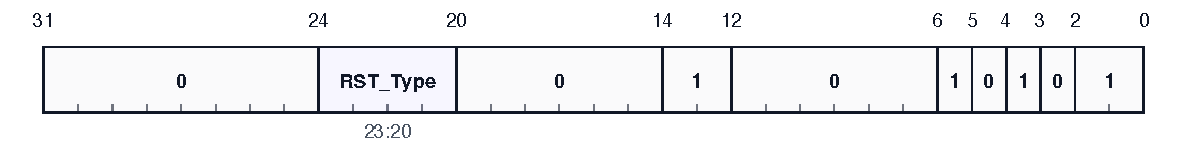
\includegraphics[width=\textwidth]{figs/encoding/scalar_instruction_entries/enc_acrc.pdf}\par\smallskip
\begin{description}[leftmargin=0.18\linewidth,style=nextline]
\item[Format] \texttt{L32} \texttt{32-bit} scalar word.
\item[Pattern] \texttt{00000000....00000011000000101011}.
\end{description}
\noindent\textbf{Classification.}\par
\begin{description}[leftmargin=0.18\linewidth,style=nextline]
\item[Category] System, Cache, SSR, and Execution Control.
\item[Family] Execution Control.
\item[Execution class] \texttt{SYS}; uop\_kind=SYS.
\end{description}
\noindent\textbf{Operand fields.}\par
\begin{description}[leftmargin=0.18\linewidth,style=nextline]
\item[\texttt{RST\_Type}] Bits \texttt{23:20 (4b)}. 4-bit architectural event-state selector used by the ACRE event-control instruction.
\end{description}
\noindent\textbf{Operation.}\par
\begin{lstlisting}[style=ptoscalarcode]
CallACR(rst_type)  // privileged ring call (implementation-defined)
\end{lstlisting}
\Needspace{0.08\textheight}

\medskip
% Scalar instruction entry source: tools/generate_scalar_instruction_catalog.py.
\subsection{\texttt{ACRE}}
\label{sec:scalar-acre}
\index{ACRE@\texttt{ACRE}}
\begin{sloppypar}\noindent\textbf{Purpose.} Architectural control operation (sub-operation selected by the operand encoding).\end{sloppypar}\smallskip
\noindent\textbf{Syntax.}\par
\begin{lstlisting}[style=ptoscalarcode]
acre rra_type
\end{lstlisting}
\noindent\textbf{Encoding.}\par
\noindent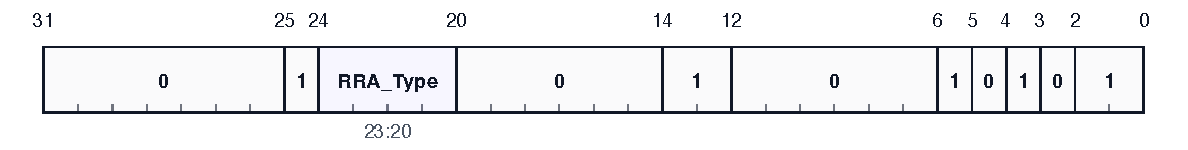
\includegraphics[width=\textwidth]{figs/encoding/scalar_instruction_entries/enc_acre.pdf}\par\smallskip
\begin{description}[leftmargin=0.18\linewidth,style=nextline]
\item[Format] \texttt{L32} \texttt{32-bit} scalar word.
\item[Pattern] \texttt{00000001....00000011000000101011}.
\end{description}
\noindent\textbf{Classification.}\par
\begin{description}[leftmargin=0.18\linewidth,style=nextline]
\item[Category] System, Cache, SSR, and Execution Control.
\item[Family] Execution Control.
\item[Execution class] \texttt{SYS}; uop\_kind=SYS.
\end{description}
\noindent\textbf{Operand fields.}\par
\begin{description}[leftmargin=0.18\linewidth,style=nextline]
\item[\texttt{RRA\_Type}] Bits \texttt{23:20 (4b)}. 4-bit architectural event-state selector used by the ACRE event-control instruction.
\end{description}
\noindent\textbf{Operation.}\par
\begin{lstlisting}[style=ptoscalarcode]
EnterACR(rra_type)  // privileged ring transition (implementation-defined)
\end{lstlisting}
\Needspace{0.08\textheight}

\medskip
\input{scalar-instructions/entries/012_assert.tex}
\medskip
% Scalar instruction entry source: tools/generate_scalar_instruction_catalog.py.
\subsection{\texttt{BC.IALL}}
\label{sec:scalar-bc_iall}
\index{BC.IALL@\texttt{BC.IALL}}
\begin{sloppypar}\noindent\textbf{Purpose.} Invalidates all branch predictor or branch-cache state defined by the scalar profile.\end{sloppypar}\smallskip
\noindent\textbf{Syntax.}\par
\begin{lstlisting}[style=ptoscalarcode]
bc.iall
\end{lstlisting}
\noindent\textbf{Encoding.}\par
\noindent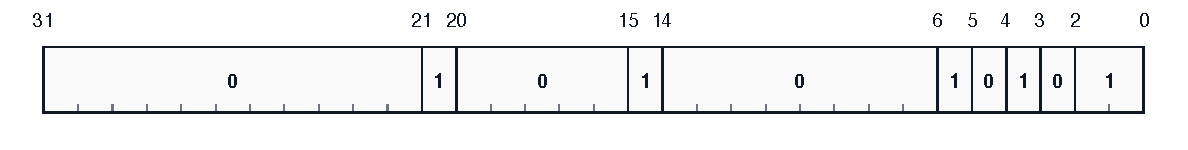
\includegraphics[width=\textwidth]{figs/encoding/scalar_instruction_entries/enc_bc_iall.pdf}\par\smallskip
\begin{description}[leftmargin=0.18\linewidth,style=nextline]
\item[Format] \texttt{L32} \texttt{32-bit} scalar word.
\item[Pattern] \texttt{00000000000100000100000000101011}.
\end{description}
\noindent\textbf{Classification.}\par
\begin{description}[leftmargin=0.18\linewidth,style=nextline]
\item[Category] System, Cache, SSR, and Execution Control.
\item[Family] Cache Maintain.
\item[Execution class] \texttt{SYS}; uop\_kind=SYS, sys\_kind=CACHE\_MAINT.
\end{description}
\noindent\textbf{Operand fields.}\par
\noindent No variable operand fields are present in this fixed encoding.\par\smallskip
\noindent\textbf{Operation.}\par
\begin{lstlisting}[style=ptoscalarcode]
Maintain(op)
\end{lstlisting}
\Needspace{0.08\textheight}

\medskip
\input{scalar-instructions/entries/022_bc_iva.tex}
\medskip
\input{scalar-instructions/entries/026_bse.tex}
\medskip
% Scalar instruction entry source: tools/generate_scalar_instruction_catalog.py.
\subsection{\texttt{BWE}}
\label{sec:scalar-bwe}
\index{BWE@\texttt{BWE}}
\begin{sloppypar}\noindent\textbf{Purpose.} Execution-control wait/event primitive (exact behavior is platform-defined).\end{sloppypar}\smallskip
\noindent\textbf{Syntax.}\par
\begin{lstlisting}[style=ptoscalarcode]
bwe SrcL
\end{lstlisting}
\noindent\textbf{Encoding.}\par
\noindent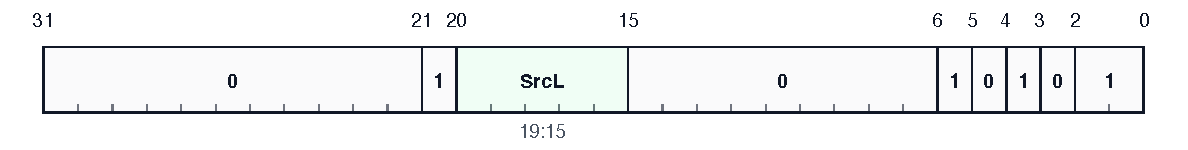
\includegraphics[width=\textwidth]{figs/encoding/scalar_instruction_entries/enc_bwe.pdf}\par\smallskip
\begin{description}[leftmargin=0.18\linewidth,style=nextline]
\item[Format] \texttt{L32} \texttt{32-bit} scalar word.
\item[Pattern] \texttt{000000000001.....000000000101011}.
\end{description}
\noindent\textbf{Classification.}\par
\begin{description}[leftmargin=0.18\linewidth,style=nextline]
\item[Category] System, Cache, SSR, and Execution Control.
\item[Family] Execution Control.
\item[Execution class] \texttt{SYS}; uop\_kind=SYS.
\end{description}
\noindent\textbf{Operand fields.}\par
\begin{description}[leftmargin=0.18\linewidth,style=nextline]
\item[\texttt{SrcL}] Bits \texttt{19:15 (5b)}. 5-bit scalar source register used as the left input operand.
\end{description}
\noindent\textbf{Operation.}\par
\begin{lstlisting}[style=ptoscalarcode]
BlockHint()  // front-end metadata; no architectural effect
\end{lstlisting}
\Needspace{0.08\textheight}

\medskip
\input{scalar-instructions/entries/028_bwi.tex}
\medskip
% Scalar instruction entry source: tools/generate_scalar_instruction_catalog.py.
\subsection{\texttt{BWT}}
\label{sec:scalar-bwt}
\index{BWT@\texttt{BWT}}
\begin{sloppypar}\noindent\textbf{Purpose.} Requests the processor to sleep for a duration specified by the operand.\end{sloppypar}\smallskip
\noindent\textbf{Syntax.}\par
\begin{lstlisting}[style=ptoscalarcode]
bwt SrcL
\end{lstlisting}
\noindent\textbf{Encoding.}\par
\noindent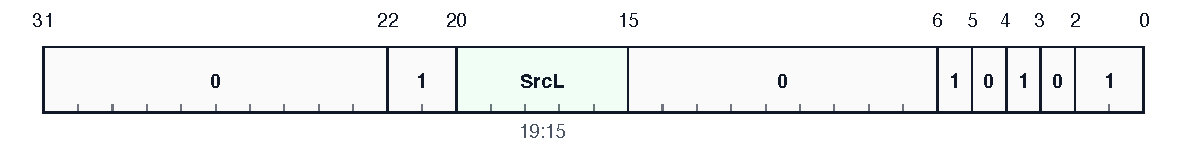
\includegraphics[width=\textwidth]{figs/encoding/scalar_instruction_entries/enc_bwt.pdf}\par\smallskip
\begin{description}[leftmargin=0.18\linewidth,style=nextline]
\item[Format] \texttt{L32} \texttt{32-bit} scalar word.
\item[Pattern] \texttt{000000000011.....000000000101011}.
\end{description}
\noindent\textbf{Classification.}\par
\begin{description}[leftmargin=0.18\linewidth,style=nextline]
\item[Category] System, Cache, SSR, and Execution Control.
\item[Family] Execution Control.
\item[Execution class] \texttt{SYS}; uop\_kind=SYS.
\end{description}
\noindent\textbf{Operand fields.}\par
\begin{description}[leftmargin=0.18\linewidth,style=nextline]
\item[\texttt{SrcL}] Bits \texttt{19:15 (5b)}. 5-bit scalar source register used as the left input operand.
\end{description}
\noindent\textbf{Operation.}\par
\begin{lstlisting}[style=ptoscalarcode]
BlockHint()  // front-end metadata; no architectural effect
\end{lstlisting}
\Needspace{0.08\textheight}

\medskip
\input{scalar-instructions/entries/051_dc_cisw.tex}
\medskip
\input{scalar-instructions/entries/052_dc_civa.tex}
\medskip
\input{scalar-instructions/entries/053_dc_csw.tex}
\medskip
\input{scalar-instructions/entries/054_dc_cva.tex}
\medskip
% Scalar instruction entry source: tools/generate_scalar_instruction_catalog.py.
\subsection{\texttt{DC.IALL}}
\label{sec:scalar-dc_iall}
\index{DC.IALL@\texttt{DC.IALL}}
\begin{sloppypar}\noindent\textbf{Purpose.} Invalidates all data-cache state defined by the scalar profile.\end{sloppypar}\smallskip
\noindent\textbf{Syntax.}\par
\begin{lstlisting}[style=ptoscalarcode]
dc.iall
\end{lstlisting}
\noindent\textbf{Encoding.}\par
\noindent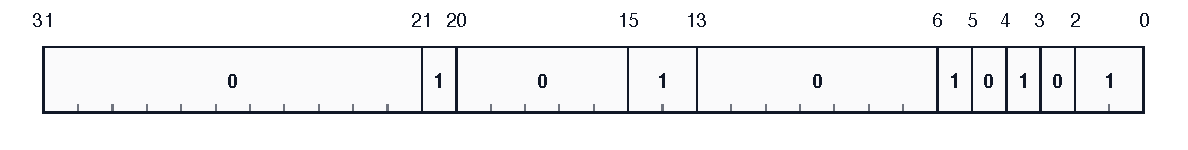
\includegraphics[width=\textwidth]{figs/encoding/scalar_instruction_entries/enc_dc_iall.pdf}\par\smallskip
\begin{description}[leftmargin=0.18\linewidth,style=nextline]
\item[Format] \texttt{L32} \texttt{32-bit} scalar word.
\item[Pattern] \texttt{00000000000100000110000000101011}.
\end{description}
\noindent\textbf{Classification.}\par
\begin{description}[leftmargin=0.18\linewidth,style=nextline]
\item[Category] System, Cache, SSR, and Execution Control.
\item[Family] Cache Maintain.
\item[Execution class] \texttt{SYS}; uop\_kind=SYS, sys\_kind=CACHE\_MAINT.
\end{description}
\noindent\textbf{Operand fields.}\par
\noindent No variable operand fields are present in this fixed encoding.\par\smallskip
\noindent\textbf{Operation.}\par
\begin{lstlisting}[style=ptoscalarcode]
Maintain(op)
\end{lstlisting}
\Needspace{0.08\textheight}

\medskip
\input{scalar-instructions/entries/056_dc_isw.tex}
\medskip
\input{scalar-instructions/entries/057_dc_iva.tex}
\medskip
\input{scalar-instructions/entries/058_dc_zva.tex}
\medskip
% Scalar instruction entry source: tools/generate_scalar_instruction_catalog.py.
\subsection{\texttt{EBREAK}}
\label{sec:scalar-ebreak}
\index{EBREAK@\texttt{EBREAK}}
\begin{sloppypar}\noindent\textbf{Purpose.} Execution-control instruction used for debugging, ordering, or bring-up.\end{sloppypar}\smallskip
\noindent\textbf{Syntax.}\par
\begin{lstlisting}[style=ptoscalarcode]
ebreak imm
\end{lstlisting}
\noindent\textbf{Encoding.}\par
\noindent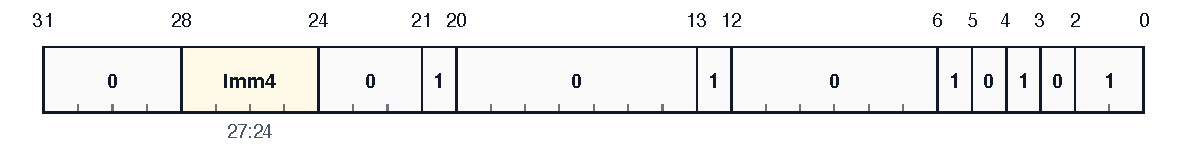
\includegraphics[width=\textwidth]{figs/encoding/scalar_instruction_entries/enc_ebreak.pdf}\par\smallskip
\begin{description}[leftmargin=0.18\linewidth,style=nextline]
\item[Format] \texttt{L32} \texttt{32-bit} scalar word.
\item[Pattern] \texttt{0000....000100000001000000101011}.
\end{description}
\noindent\textbf{Classification.}\par
\begin{description}[leftmargin=0.18\linewidth,style=nextline]
\item[Category] System, Cache, SSR, and Execution Control.
\item[Family] Execution Control.
\item[Execution class] \texttt{SYS}; uop\_kind=SYS.
\end{description}
\noindent\textbf{Operand fields.}\par
\begin{description}[leftmargin=0.18\linewidth,style=nextline]
\item[\texttt{imm4}] Bits \texttt{27:24 (4b)}. 4-bit unsigned immediate operand consumed directly by the operation.
\end{description}
\noindent\textbf{Operation.}\par
\begin{lstlisting}[style=ptoscalarcode]
Trap(SW_BREAKPOINT)
\end{lstlisting}
\Needspace{0.08\textheight}

\medskip
% Scalar instruction entry source: tools/generate_scalar_instruction_catalog.py.
\subsection{\texttt{FENCE.D}}
\label{sec:scalar-fence_d}
\index{FENCE.D@\texttt{FENCE.D}}
\begin{sloppypar}\noindent\textbf{Purpose.} Orders data-memory operations according to the encoded predecessor and successor masks.\end{sloppypar}\smallskip
\noindent\textbf{Syntax.}\par
\begin{lstlisting}[style=ptoscalarcode]
fence.d pred_imm, succ_imm
\end{lstlisting}
\noindent\textbf{Encoding.}\par
\noindent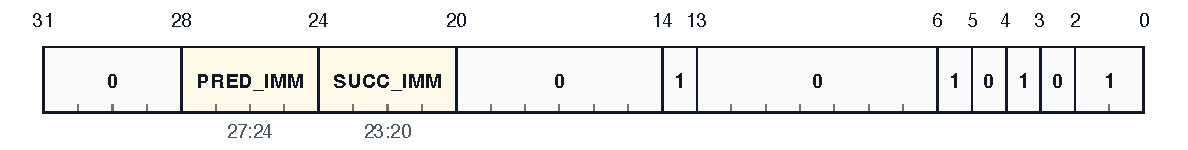
\includegraphics[width=\textwidth]{figs/encoding/scalar_instruction_entries/enc_fence_d.pdf}\par\smallskip
\begin{description}[leftmargin=0.18\linewidth,style=nextline]
\item[Format] \texttt{L32} \texttt{32-bit} scalar word.
\item[Pattern] \texttt{0000........00000010000000101011}.
\end{description}
\noindent\textbf{Classification.}\par
\begin{description}[leftmargin=0.18\linewidth,style=nextline]
\item[Category] System, Cache, SSR, and Execution Control.
\item[Family] Execution Control.
\item[Execution class] \texttt{SYS}; uop\_kind=SYS.
\end{description}
\noindent\textbf{Operand fields.}\par
\begin{description}[leftmargin=0.18\linewidth,style=nextline]
\item[\texttt{PRED\_IMM}] Bits \texttt{27:24 (4b)}. 4-bit fence predecessor set. Each bit names a memory or I/O access class participating in the ordering constraint.
\item[\texttt{SUCC\_IMM}] Bits \texttt{23:20 (4b)}. 4-bit fence successor set. Each bit names a memory or I/O access class participating in the ordering constraint.
\end{description}
\noindent\textbf{Operation.}\par
\begin{lstlisting}[style=ptoscalarcode]
FenceD()  // data-cache fence
\end{lstlisting}
\Needspace{0.08\textheight}

\medskip
% Scalar instruction entry source: tools/generate_scalar_instruction_catalog.py.
\subsection{\texttt{FENCE.I}}
\label{sec:scalar-fence_i}
\index{FENCE.I@\texttt{FENCE.I}}
\begin{sloppypar}\noindent\textbf{Purpose.} Synchronizes instruction fetch with prior stores to instruction memory for the current execution context.\end{sloppypar}\smallskip
\noindent\textbf{Syntax.}\par
\begin{lstlisting}[style=ptoscalarcode]
fence.i
\end{lstlisting}
\noindent\textbf{Encoding.}\par
\noindent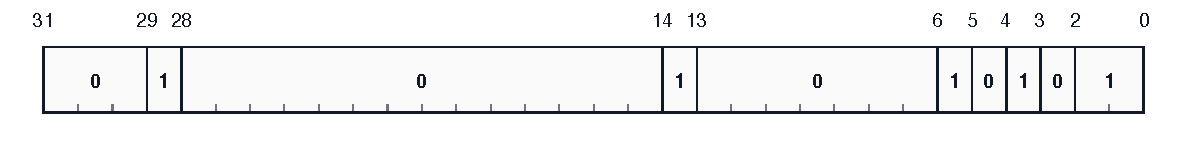
\includegraphics[width=\textwidth]{figs/encoding/scalar_instruction_entries/enc_fence_i.pdf}\par\smallskip
\begin{description}[leftmargin=0.18\linewidth,style=nextline]
\item[Format] \texttt{L32} \texttt{32-bit} scalar word.
\item[Pattern] \texttt{00010000000000000010000000101011}.
\end{description}
\noindent\textbf{Classification.}\par
\begin{description}[leftmargin=0.18\linewidth,style=nextline]
\item[Category] System, Cache, SSR, and Execution Control.
\item[Family] Execution Control.
\item[Execution class] \texttt{SYS}; uop\_kind=SYS.
\end{description}
\noindent\textbf{Operand fields.}\par
\noindent No variable operand fields are present in this fixed encoding.\par\smallskip
\noindent\textbf{Operation.}\par
\begin{lstlisting}[style=ptoscalarcode]
FenceI()  // instruction-cache fence
\end{lstlisting}
\Needspace{0.08\textheight}

\medskip
% Scalar instruction entry source: tools/generate_scalar_instruction_catalog.py.
\subsection{\texttt{IC.IALL}}
\label{sec:scalar-ic_iall}
\index{IC.IALL@\texttt{IC.IALL}}
\begin{sloppypar}\noindent\textbf{Purpose.} Invalidates all instruction-cache state defined by the scalar profile.\end{sloppypar}\smallskip
\noindent\textbf{Syntax.}\par
\begin{lstlisting}[style=ptoscalarcode]
ic.iall
\end{lstlisting}
\noindent\textbf{Encoding.}\par
\noindent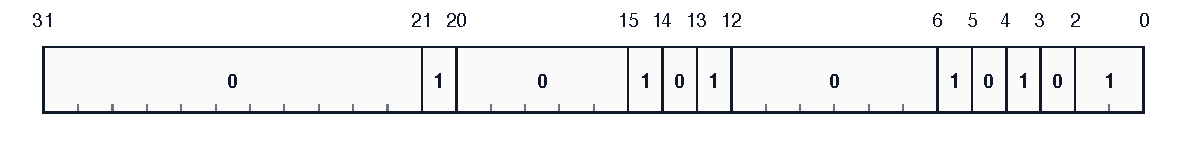
\includegraphics[width=\textwidth]{figs/encoding/scalar_instruction_entries/enc_ic_iall.pdf}\par\smallskip
\begin{description}[leftmargin=0.18\linewidth,style=nextline]
\item[Format] \texttt{L32} \texttt{32-bit} scalar word.
\item[Pattern] \texttt{00000000000100000101000000101011}.
\end{description}
\noindent\textbf{Classification.}\par
\begin{description}[leftmargin=0.18\linewidth,style=nextline]
\item[Category] System, Cache, SSR, and Execution Control.
\item[Family] Cache Maintain.
\item[Execution class] \texttt{SYS}; uop\_kind=SYS, sys\_kind=CACHE\_MAINT.
\end{description}
\noindent\textbf{Operand fields.}\par
\noindent No variable operand fields are present in this fixed encoding.\par\smallskip
\noindent\textbf{Operation.}\par
\begin{lstlisting}[style=ptoscalarcode]
Maintain(op)
\end{lstlisting}
\Needspace{0.08\textheight}

\medskip
\input{scalar-instructions/entries/095_ic_iva.tex}
\medskip
% Scalar instruction entry source: tools/generate_scalar_instruction_catalog.py.
\subsection{\texttt{LSRGET}}
\label{sec:scalar-lsrget}
\index{LSRGET@\texttt{LSRGET}}
\begin{sloppypar}\noindent\textbf{Purpose.} Reads a system register identified by the ID operand and writes the value to the selected destination.\end{sloppypar}\smallskip
\noindent\textbf{Syntax.}\par
\begin{lstlisting}[style=ptoscalarcode]
lsrget LSR_ID, ->RegDst
\end{lstlisting}
\noindent\textbf{Encoding.}\par
\noindent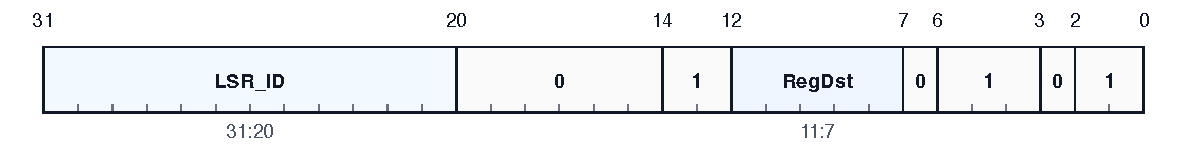
\includegraphics[width=\textwidth]{figs/encoding/scalar_instruction_entries/enc_lsrget.pdf}\par\smallskip
\begin{description}[leftmargin=0.18\linewidth,style=nextline]
\item[Format] \texttt{L32} \texttt{32-bit} scalar word.
\item[Pattern] \texttt{............00000011.....0111011}.
\end{description}
\noindent\textbf{Classification.}\par
\begin{description}[leftmargin=0.18\linewidth,style=nextline]
\item[Category] System, Cache, SSR, and Execution Control.
\item[Family] SSR Access.
\item[Execution class] \texttt{SYS}; uop\_kind=SYS, sys\_kind=SSR.
\end{description}
\noindent\textbf{Operand fields.}\par
\begin{description}[leftmargin=0.18\linewidth,style=nextline]
\item[\texttt{LSR\_ID}] Bits \texttt{31:20 (12b)}. 12-bit local/system register identifier selected by this register-access instruction.
\item[\texttt{RegDst}] Bits \texttt{11:7 (5b)}. 5-bit scalar destination register that receives the loaded value after any sign or zero extension; X0 discards the load result.
\end{description}
\noindent\textbf{Operation.}\par
\begin{lstlisting}[style=ptoscalarcode]
value = ReadSystemRegister(ID)
Write(RegDst, value)
\end{lstlisting}
\Needspace{0.08\textheight}

\medskip
% Scalar instruction entry source: tools/generate_scalar_instruction_catalog.py.
\subsection{\texttt{SETC.TGT}}
\label{sec:scalar-setc_tgt}
\index{SETC.TGT@\texttt{SETC.TGT}}
\begin{sloppypar}\noindent\textbf{Purpose.} Sets the block-commit condition/argument consumed by subsequent conditional block transitions.\end{sloppypar}\smallskip
\noindent\textbf{Syntax.}\par
\begin{lstlisting}[style=ptoscalarcode]
setc.tgt SrcL
\end{lstlisting}
\noindent\textbf{Encoding.}\par
\noindent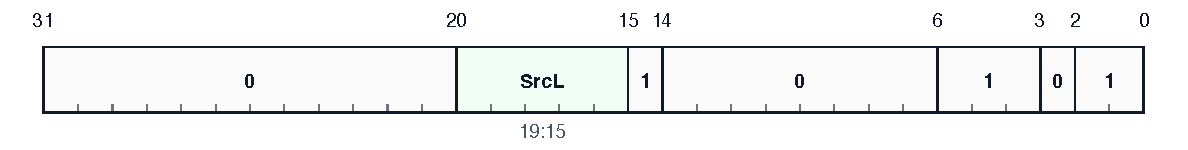
\includegraphics[width=\textwidth]{figs/encoding/scalar_instruction_entries/enc_setc_tgt.pdf}\par\smallskip
\begin{description}[leftmargin=0.18\linewidth,style=nextline]
\item[Format] \texttt{L32} \texttt{32-bit} scalar word.
\item[Pattern] \texttt{000000000000.....100000000111011}.
\end{description}
\noindent\textbf{Classification.}\par
\begin{description}[leftmargin=0.18\linewidth,style=nextline]
\item[Category] System, Cache, SSR, and Execution Control.
\item[Family] SSR Access.
\item[Execution class] \texttt{SYS}; uop\_kind=SYS, sys\_kind=SSR.
\end{description}
\noindent\textbf{Operand fields.}\par
\begin{description}[leftmargin=0.18\linewidth,style=nextline]
\item[\texttt{SrcL}] Bits \texttt{19:15 (5b)}. 5-bit scalar source register used as the left input operand.
\end{description}
\noindent\textbf{Operation.}\par
\begin{lstlisting}[style=ptoscalarcode]
SetCommitTarget(Read(SrcL))
\end{lstlisting}
\Needspace{0.08\textheight}

\medskip
% Scalar instruction entry source: tools/generate_scalar_instruction_catalog.py.
\subsection{\texttt{SSRGET}}
\label{sec:scalar-ssrget}
\index{SSRGET@\texttt{SSRGET}}
\begin{sloppypar}\noindent\textbf{Purpose.} Reads a system register identified by the ID operand and writes the value to the selected destination.\end{sloppypar}\smallskip
\noindent\textbf{Syntax.}\par
\begin{lstlisting}[style=ptoscalarcode]
ssrget SSR_ID, ->RegDst
\end{lstlisting}
\noindent\textbf{Encoding.}\par
\noindent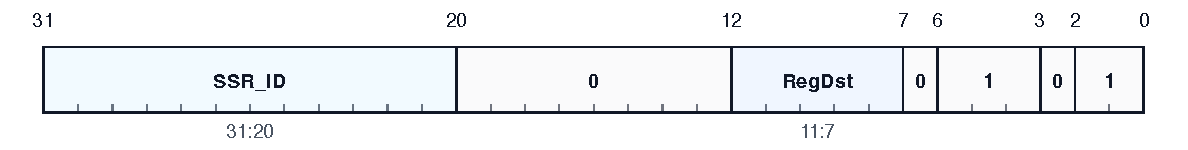
\includegraphics[width=\textwidth]{figs/encoding/scalar_instruction_entries/enc_ssrget.pdf}\par\smallskip
\begin{description}[leftmargin=0.18\linewidth,style=nextline]
\item[Format] \texttt{L32} \texttt{32-bit} scalar word.
\item[Pattern] \texttt{............00000000.....0111011}.
\end{description}
\noindent\textbf{Classification.}\par
\begin{description}[leftmargin=0.18\linewidth,style=nextline]
\item[Category] System, Cache, SSR, and Execution Control.
\item[Family] SSR Access.
\item[Execution class] \texttt{SYS}; uop\_kind=SYS, sys\_kind=SSR.
\end{description}
\noindent\textbf{Operand fields.}\par
\begin{description}[leftmargin=0.18\linewidth,style=nextline]
\item[\texttt{RegDst}] Bits \texttt{11:7 (5b)}. 5-bit scalar destination register written by this instruction; X0 is hardwired to zero, so writes to X0 are ignored.
\item[\texttt{SSR\_ID}] Bits \texttt{31:20 (12b)}. 12-bit system scalar register identifier selecting the SSR read, write, set, or swap target.
\end{description}
\noindent\textbf{Operation.}\par
\begin{lstlisting}[style=ptoscalarcode]
value = ReadSystemRegister(ID)
Write(RegDst, value)
\end{lstlisting}
\Needspace{0.08\textheight}

\medskip
% Scalar instruction entry source: tools/generate_scalar_instruction_catalog.py.
\subsection{\texttt{SSRSET}}
\label{sec:scalar-ssrset}
\index{SSRSET@\texttt{SSRSET}}
\begin{sloppypar}\noindent\textbf{Purpose.} Writes a system register identified by the ID operand with the provided value.\end{sloppypar}\smallskip
\noindent\textbf{Syntax.}\par
\begin{lstlisting}[style=ptoscalarcode]
ssrset SrcL, SSR_ID
\end{lstlisting}
\noindent\textbf{Encoding.}\par
\noindent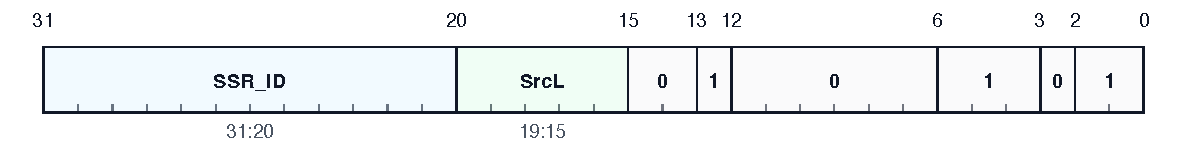
\includegraphics[width=\textwidth]{figs/encoding/scalar_instruction_entries/enc_ssrset.pdf}\par\smallskip
\begin{description}[leftmargin=0.18\linewidth,style=nextline]
\item[Format] \texttt{L32} \texttt{32-bit} scalar word.
\item[Pattern] \texttt{.................001000000111011}.
\end{description}
\noindent\textbf{Classification.}\par
\begin{description}[leftmargin=0.18\linewidth,style=nextline]
\item[Category] System, Cache, SSR, and Execution Control.
\item[Family] SSR Access.
\item[Execution class] \texttt{SYS}; uop\_kind=SYS, sys\_kind=SSR.
\end{description}
\noindent\textbf{Operand fields.}\par
\begin{description}[leftmargin=0.18\linewidth,style=nextline]
\item[\texttt{SSR\_ID}] Bits \texttt{31:20 (12b)}. 12-bit system scalar register identifier selecting the SSR read, write, set, or swap target.
\item[\texttt{SrcL}] Bits \texttt{19:15 (5b)}. 5-bit scalar source register used as the left input operand.
\end{description}
\noindent\textbf{Operation.}\par
\begin{lstlisting}[style=ptoscalarcode]
WriteSystemRegister(ID, Read(SrcL))
\end{lstlisting}
\Needspace{0.08\textheight}

\medskip
% Scalar instruction entry source: tools/generate_scalar_instruction_catalog.py.
\subsection{\texttt{SSRSWAP}}
\label{sec:scalar-ssrswap}
\index{SSRSWAP@\texttt{SSRSWAP}}
\begin{sloppypar}\noindent\textbf{Purpose.} Atomically swaps a system register value with the provided value.\end{sloppypar}\smallskip
\noindent\textbf{Syntax.}\par
\begin{lstlisting}[style=ptoscalarcode]
ssrswap SrcL, SSR_ID, ->RegDst
\end{lstlisting}
\noindent\textbf{Encoding.}\par
\noindent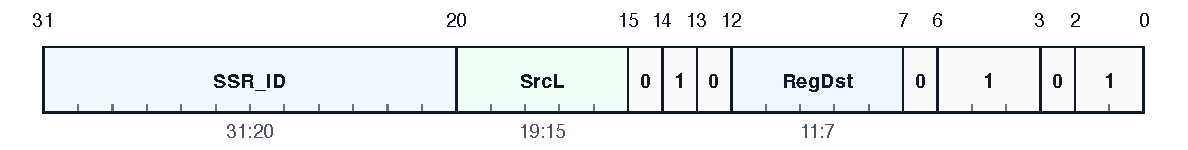
\includegraphics[width=\textwidth]{figs/encoding/scalar_instruction_entries/enc_ssrswap.pdf}\par\smallskip
\begin{description}[leftmargin=0.18\linewidth,style=nextline]
\item[Format] \texttt{L32} \texttt{32-bit} scalar word.
\item[Pattern] \texttt{.................010.....0111011}.
\end{description}
\noindent\textbf{Classification.}\par
\begin{description}[leftmargin=0.18\linewidth,style=nextline]
\item[Category] System, Cache, SSR, and Execution Control.
\item[Family] SSR Access.
\item[Execution class] \texttt{SYS}; uop\_kind=SYS, sys\_kind=SSR.
\end{description}
\noindent\textbf{Operand fields.}\par
\begin{description}[leftmargin=0.18\linewidth,style=nextline]
\item[\texttt{RegDst}] Bits \texttt{11:7 (5b)}. 5-bit scalar destination register written by this instruction; X0 is hardwired to zero, so writes to X0 are ignored.
\item[\texttt{SSR\_ID}] Bits \texttt{31:20 (12b)}. 12-bit system scalar register identifier selecting the SSR read, write, set, or swap target.
\item[\texttt{SrcL}] Bits \texttt{19:15 (5b)}. 5-bit scalar source register used as the left input operand.
\end{description}
\noindent\textbf{Operation.}\par
\begin{lstlisting}[style=ptoscalarcode]
old = ReadSystemRegister(ID)
WriteSystemRegister(ID, Read(SrcL))
Write(RegDst, old)
\end{lstlisting}
\Needspace{0.08\textheight}

\medskip
% Scalar instruction entry source: tools/generate_scalar_instruction_catalog.py.
\subsection{\texttt{TLB.IA}}
\label{sec:scalar-tlb_ia}
\index{TLB.IA@\texttt{TLB.IA}}
\begin{sloppypar}\noindent\textbf{Purpose.} Invalidates address-translation state for the supplied address operand.\end{sloppypar}\smallskip
\noindent\textbf{Syntax.}\par
\begin{lstlisting}[style=ptoscalarcode]
tlb.ia SrcL
\end{lstlisting}
\noindent\textbf{Encoding.}\par
\noindent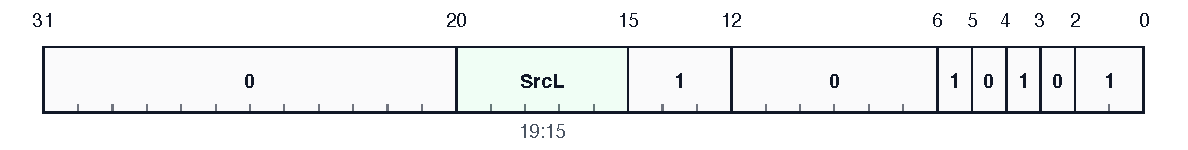
\includegraphics[width=\textwidth]{figs/encoding/scalar_instruction_entries/enc_tlb_ia.pdf}\par\smallskip
\begin{description}[leftmargin=0.18\linewidth,style=nextline]
\item[Format] \texttt{L32} \texttt{32-bit} scalar word.
\item[Pattern] \texttt{000000000000.....111000000101011}.
\end{description}
\noindent\textbf{Classification.}\par
\begin{description}[leftmargin=0.18\linewidth,style=nextline]
\item[Category] System, Cache, SSR, and Execution Control.
\item[Family] Cache Maintain.
\item[Execution class] \texttt{SYS}; uop\_kind=SYS, sys\_kind=CACHE\_MAINT.
\end{description}
\noindent\textbf{Operand fields.}\par
\begin{description}[leftmargin=0.18\linewidth,style=nextline]
\item[\texttt{SrcL}] Bits \texttt{19:15 (5b)}. 5-bit scalar source register supplying the address or selector operand for this maintenance operation.
\end{description}
\noindent\textbf{Operation.}\par
\begin{lstlisting}[style=ptoscalarcode]
Maintain(op, address=Read(SrcL))
\end{lstlisting}
\Needspace{0.08\textheight}

\medskip
% Scalar instruction entry source: tools/generate_scalar_instruction_catalog.py.
\subsection{\texttt{TLB.IALL}}
\label{sec:scalar-tlb_iall}
\index{TLB.IALL@\texttt{TLB.IALL}}
\begin{sloppypar}\noindent\textbf{Purpose.} Invalidates all address-translation state defined by the scalar profile.\end{sloppypar}\smallskip
\noindent\textbf{Syntax.}\par
\begin{lstlisting}[style=ptoscalarcode]
tlb.iall
\end{lstlisting}
\noindent\textbf{Encoding.}\par
\noindent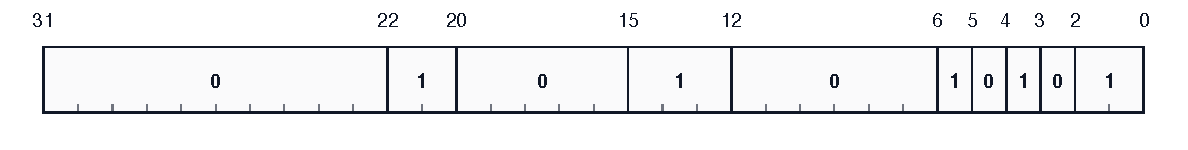
\includegraphics[width=\textwidth]{figs/encoding/scalar_instruction_entries/enc_tlb_iall.pdf}\par\smallskip
\begin{description}[leftmargin=0.18\linewidth,style=nextline]
\item[Format] \texttt{L32} \texttt{32-bit} scalar word.
\item[Pattern] \texttt{00000000001100000111000000101011}.
\end{description}
\noindent\textbf{Classification.}\par
\begin{description}[leftmargin=0.18\linewidth,style=nextline]
\item[Category] System, Cache, SSR, and Execution Control.
\item[Family] Cache Maintain.
\item[Execution class] \texttt{SYS}; uop\_kind=SYS, sys\_kind=CACHE\_MAINT.
\end{description}
\noindent\textbf{Operand fields.}\par
\noindent No variable operand fields are present in this fixed encoding.\par\smallskip
\noindent\textbf{Operation.}\par
\begin{lstlisting}[style=ptoscalarcode]
Maintain(op)
\end{lstlisting}
\Needspace{0.08\textheight}

\medskip
\input{scalar-instructions/entries/233_tlb_iav.tex}
\medskip
% Scalar instruction entry source: tools/generate_scalar_instruction_catalog.py.
\subsection{\texttt{TLB.IV}}
\label{sec:scalar-tlb_iv}
\index{TLB.IV@\texttt{TLB.IV}}
\begin{sloppypar}\noindent\textbf{Purpose.} Invalidates virtual-address translation state selected by the encoded operand.\end{sloppypar}\smallskip
\noindent\textbf{Syntax.}\par
\begin{lstlisting}[style=ptoscalarcode]
tlb.iv SrcL
\end{lstlisting}
\noindent\textbf{Encoding.}\par
\noindent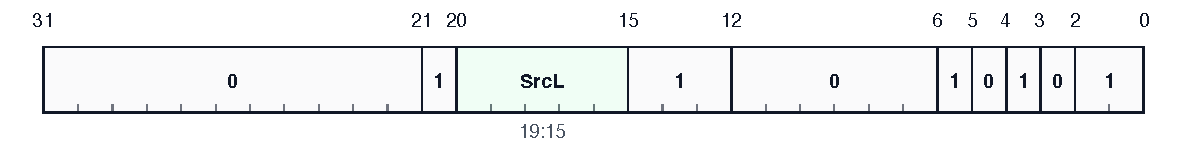
\includegraphics[width=\textwidth]{figs/encoding/scalar_instruction_entries/enc_tlb_iv.pdf}\par\smallskip
\begin{description}[leftmargin=0.18\linewidth,style=nextline]
\item[Format] \texttt{L32} \texttt{32-bit} scalar word.
\item[Pattern] \texttt{000000000001.....111000000101011}.
\end{description}
\noindent\textbf{Classification.}\par
\begin{description}[leftmargin=0.18\linewidth,style=nextline]
\item[Category] System, Cache, SSR, and Execution Control.
\item[Family] Cache Maintain.
\item[Execution class] \texttt{SYS}; uop\_kind=SYS, sys\_kind=CACHE\_MAINT.
\end{description}
\noindent\textbf{Operand fields.}\par
\begin{description}[leftmargin=0.18\linewidth,style=nextline]
\item[\texttt{SrcL}] Bits \texttt{19:15 (5b)}. 5-bit scalar source register supplying the address or selector operand for this maintenance operation.
\end{description}
\noindent\textbf{Operation.}\par
\begin{lstlisting}[style=ptoscalarcode]
Maintain(op, address=Read(SrcL))
\end{lstlisting}
\Needspace{0.08\textheight}

\medskip
